\documentclass[12pt, a4paper]{report}
\special{papersize=210mm, 297mm}
\usepackage[english]{babel}
\usepackage[utf8x]{inputenc}
\usepackage[left=2.5cm, right=2.5cm, top=2.5cm]{geometry}
\renewcommand{\baselinestretch}{1.4}
\usepackage[toc,page]{appendix}

\usepackage{amsmath}
\usepackage{graphicx}
\usepackage{float}
\graphicspath{{images/} {diagrams/}}

%\usepackage{showframe}
\usepackage{fullpage}

\usepackage{url}
%\usepackage{natbib} % for author-date citation \citep{}, \citet[]
%\usepackage{hyperref}
%\usepackage[nottoc]{tocbibind}
\usepackage{listings}
\usepackage{verbatim}
\usepackage{color}

\definecolor{dkgreen}{rgb}{0,0.6,0}
\definecolor{gray}{rgb}{0.5,0.5,0.5}
\definecolor{mauve}{rgb}{0.58,0,0.82}

\lstset{frame=tb,
	language=java,
	aboveskip=5mm, belowskip=3mm, showstringspaces=false,
	columns=flexible, basicstyle={\small\ttfamily},
	numbers=none, numberstyle=\tiny\color{gray},
	keywordstyle=\color{blue},
	commentstyle=\color{dkgreen},
	stringstyle=\color{mauve},
	breaklines=true,
	breakatwhitespace=true,
	tabsize=3
}


\usepackage{multirow}
\usepackage{array}
\newcolumntype{L}[1]{> {\raggedright\let\newline\\\arraybackslash\hspace{0pt}}m{#1}}
\newcolumntype{C}[1]{>{\centering\let\newline\\\arraybackslash\hspace{0pt}}m{#1}}
\newcolumntype{R}[1]{>{\raggedleft\let\newline\\\arraybackslash\hspace{0pt}}m{#1}}

\pagenumbering{roman}

\begin{document}
	
	%======================================================================
	
	\begin{titlepage}
		
		\newcommand{\HRule}{\rule{\linewidth}{0.5mm}} % Defines a new command for the horizontal lines, change thickness here
		
		\center % Center everything on the page
		
		%----------------------------------------------------------------------------------------
		%	LOGO SECTION
		%----------------------------------------------------------------------------------------
		
		\vspace{-20pt}
		
\includegraphics[width=100pt]{FMI-03.png}\\[1.0cm] % Include a department/university logo - this will require the graphicx package
		
		\textsc{\LARGE West University of  Timisoara}\\[0.5cm] % Name of your university/college
		\textsc{\Large Faculty of Mathematics and Computer Science}\\[0.5cm] % Major heading such as course name
		\textsc{\large Study Program: \\Compter Science in English}\\[3cm] % Minor heading such as course title
		
		%----------------------------------------------------------------------------------------
		%	TITLE SECTION
		%----------------------------------------------------------------------------------------
		
		\textsc{\Huge Bachelor Thesis}\\[5cm]
		
		%\HRule \\[0.5cm]
		%{\huge \bfseries Simplified Transport Layer Security}
		%\\[0.4cm]
		%{\huge \bf implementation}\\[3cm] % Title of your document
		%\HRule \\[1.5cm]
		
		%----------------------------------------------------------------------------------------
		%	AUTHOR SECTION
		%----------------------------------------------------------------------------------------
		
		%\textsc{\huge Intermediate Report}
		
		\begin{minipage}{0.4\textwidth}
			\begin{flushleft} \large
				\textbf{COORDINATOR:}\\
				Associate Prof. Marc Eduard \textsc{Frîncu} % Coordinator
			\end{flushleft}
		\end{minipage}
		~
		\begin{minipage}{0.4\textwidth}
			\begin{flushright} \large
				\textbf{GRADUATE:} \\
				Maria Minerva \textsc{Vonica} % Student's Name
			\end{flushright}
		\end{minipage}\\[0.5cm]
		
		
		%----------------------------------------------------------------------------------------
		%	DATE SECTION
		%----------------------------------------------------------------------------------------
		\vfill
		{\large Timi\c{s}oara \\2019}\\ % Date, change the \today to a set date if you want to be precise
		
		
		%----------------------------------------------------------------------------------------
		
		%\vfill % Fill the rest of the page with whitespace
		
	\end{titlepage}
	
	% =====================================================================
	
	% second title page. as requested by UVT
	
	\begin{titlepage}
		
		\newcommand{\HRule}{\rule{\linewidth}{0.5mm}} % Defines a new command for the horizontal lines, change thickness here
		
		\center % Center everything on the page
		
		%----------------------------------------------------------------------------------------
		%	LOGO SECTION
		%----------------------------------------------------------------------------------------
		
		\textsc{}\\[.7cm]
		%
\includegraphics[width=100pt]{FMI-03.png}\\[1.0cm] % Include a department/university logo - this will require the graphicx package
		
		
		\textsc{\LARGE West University of  Timi\c{s}oara}\\[0.5cm] % Name of your university/college
		\textsc{\Large Faculty of Mathematics and Computer Science}\\[0.5cm] % Major heading such as course name
		\textsc{\large Study Program: \\Compter Science in English}\\[4.5cm] % Minor heading such as course title
		
		
		%----------------------------------------------------------------------------------------
		%	TITLE SECTION
		%----------------------------------------------------------------------------------------
		
		%\textsc{\Huge Master Dissertation}\\[2cm]
		
		%\HRule \\[0.5cm]
		%\HRule \\[0.5cm]
		{\Huge \bfseries Image alignment and glacier change prediction on satellite images using artificial inteligence}\\[6cm] % Title of your document
		%\HRule \\[1.5cm]
		
		%----------------------------------------------------------------------------------------
		%	AUTHOR SECTION
		%----------------------------------------------------------------------------------------
		
		%\textsc{\huge Intermediate Report}
		
		\begin{minipage}{0.4\textwidth}
			\begin{flushleft} \large
				\textbf{COORDINATOR:}\\
				Associate Prof. Marc Eduard \textsc{Frîncu} % Coordinator
			\end{flushleft}
		\end{minipage}
		~
		\begin{minipage}{0.4\textwidth}
			\begin{flushright} \large
				\textbf{GRADUATE:} \\
				Maria Minerva \textsc{Vonica} % Student's Name
			\end{flushright}
		\end{minipage}\\[0.5cm]
		
		%----------------------------------------------------------------------------------------
		%	DATE SECTION
		%----------------------------------------------------------------------------------------
		\vfill
		{\large Timi\c{s}oara\\ 2019}\\ % Date, change the \today to a set date if you want to be precise
		
		
		%----------------------------------------------------------------------------------------
		
		%\vfill % Fill the rest of the page with whitespace
		
	\end{titlepage}
	
	\begin{abstract} %begin abstract  
		%The abstract should have one page and should be a compact presentation of the dissertation.
		\vspace{1.0cm}
		\vspace{1.0cm}
		\par
		Climate change has become one of the biggest threats the world has to deal with in the near future, and yet, there is still not enough information to completely understand the phenomenon, how fast it grows and the chain reactions it will imply given that not enough measures are taken in time. Given that glaciers are the most sensitive indicators of climate change, a solution to widening the information field about the phenomenon is implementing a model of prediction on satellite images for analyzing the changes in snow coverage on glaciers during a period of over a decade and all around the globe.
		\vskip 0.2cm
		Building this application had the goal to create a tool for gathering valuable data on how fast the climate change happens by analysing the downfall of snow coverage on glaciers during a period of time and predicting by how much they will continue to shrink in the near future. Since more information means a better understanding of the phenomenon, we also made simple to use and easy to access for anyone who wants to get involved and make a contribution.
		\vskip 0.2cm
		This paper contains information on the area of analysis, the application's structure and processing mechanics. The idea is to give the users an option to easily access and download satellite data to work on, then process it by calculating the NDSI (Normalized Difference Snow Index) in order to highlight the snow on the glaciers, generating a number representing the snow ratio in each scene. By having a sample of images of a glacier taken during a big number of years and analyzing its changes in snowfall, we can see then analyze and predict the future changes over the next period, based on the snow coverage ratio for each image. Optical flow and image substracting will be applied to highlight the changes visual wise. 
		
	\end{abstract} %end abstract
	
	\tableofcontents{}
	\addcontentsline{toc}{chapter}{List Of Figures}
	\listoffigures{}
	\addcontentsline{toc}{chapter}{List Of Tables}
	\listoftables{}
	
	\newpage{}
	
	\chapter{Introduction} 
	
	Since the creation of the first Earth observation satellites, a gate to new opportunities of better understanding our planet and its behaviour has opened. The intent of the Earth observation programs is to monitor changes such as weather behavior, climate change, astronomical photography, vegetation states, droughts, earthquakes or other natural disasters, such that by analyzing the collected images, patterns which lead to understanding the cause of the behaviour are found. In order to be able to have a clear understanding of those behaviours, massive amounts of data need to be collected, organised and processed. With the large number of observation satellites orbiting the atmosphere and collecting massive amounts of data daily, deep analysis of the data sets must be done.
	
	Nowadays, one of the most important problems on a global scale is climate change, which threatens to definitely change the human life as it is known today. The changes in weather patterns, sea levels, weather events and greenhouse effects are more and more common, which will lead to permanent damage to the environment, society and human life overall.
	
	Given that the tools of understanding changes over the past years have been created with the launching of the first observation satellites in the orbit, all these changes can be tracked and predicted, so the dangerous effects of climate change and other disastrous events can be lowered.
	We have the tools to understand events which happened in the past, so we can create a safer, more balanced, and predictable future.
	
	\pagenumbering{arabic}
	\setcounter{page}{1}
	
	
	\section{Motivation and goals} 
	
	The motivation of elaborating this thesis is based on the context of the impact the climate change will have on life if not enough measures are taken and there is not enough understanding of it, as well as the availability of massive amounts of data which consists of satellite images from almost a decade back (Landsat 8 launched in 2013), and a world glacier inventory dating form 2012.
	The main reasons for elaborating a thesis on this theme are:
	\begin{itemize}
		\item The threats the climate change actually imply if not enough measures are taken as soon as possible;
		\item The possibility to better understand this phenomenon by analyzing satellite images which contain useful information;
		\item The availability of massive amounts of data which consists of satellite images from almost a decade back (Landsat8 launched in February 2013).
	\end{itemize}

	The \textbf{goal} of the thesis is to analyze satellite images focusing on changes in glaciers and snow in order to get a better overview of the changes in the environment in the last decade. 
	
	
	\section{The context of this thesis} 
	
	 Climate change has become one of the biggest problems in the past years, human activities being one of the main factors by inducing global warming \cite{climate_change_1}. Due to heavy industrialisation of the society since the Industrial Revolution around the VII century, the levels of carbon dioxide in the atmosphere have grown beyond the capacity of natural elimination, creating the greenhouse effect. 
	
	The greenhouse effect is the process in which the radiation from a planet's atmosphere warms the planet surface above that normal temperature \cite{greenhouse}. The main causes of this change are human activities such as combustion of fossil fuels (coal, oil, natural gas), deforestation, soil erosion and agriculture \cite{climate_change_2}. If the change continues at this rate, there is an estimation that the average surface temperature will surpass \textdegree{3}  C this century \cite{climate_change_3}. Though it may not seem a lot, there is a scenario created over 30 years into the future explaining what this increase actually means: from 2020 to 2030 the temperature is set to rise above \textdegree{1.6}C; by this report, it is estimated that the average temperature will increase with \textdegree{3}C around 2050, in which case even if gas emissions are stopped, there will be another rise of at least \textdegree{1}C \cite{climate_change_4}. 
	
	One of the ways of creating an overview of the last decades of climate change is by analysing the change in the glaciers, since they are among the most sensitive indicators of climate change \cite{glacier_1}. The retreat of a glacier is caused by an increase of the temperature and less snowfall, a process which has been accelerated recently, due to the global warming \cite{glacier_2}.
	
	In the context of these changes, which are already beginning to impact the society and environment, I strongly believe that we have to take advantage of every opportunity to better understand and predict these changes, so proper preparations and actions could be taken as soon as possible. 
	
	
	\section{Our Contribution}
	
	This paper uses image analysis techniques paired with artificial intelligent algorithms to create a time series analysis on the snow coverage of glaciers around the globe, while using methods which prove to be highly performant and accurate:
	\begin{itemize}
		\item Alignment of images with accuracy rate of \textbf{98\%} percent for the successful processed ones;
		\item Successful alignment of approximately \textbf{85\%} images for a Landsat 8 iamge;
		\item Snow coverage prediction with approximate \textbf{20\%} mean error.
	\end{itemize}.
	The results were achieved by calculating the NDSI for extracting snow pixels from a Landsat 8 image on a set of images for a glacier which has been split into path and row coordinates, paired up with alignment of the resulting images for displaying their differences over the years. The Normalized Difference Snow Index (NDSI) was obtained by calculating a formula which uses the green and SWIR1 bands from a scene and applying a threshold in order detect snow. The method of snow extraction was chosen to be NDSI calculation due to snow's high reflectance in the visible spectrum and high absorption in the short-wave infrared one. 
	\vskip 0.2cm
	After the snow coverage has been extracted, the NDSI, green and SWIR1 images are aligned based on a reference image, such that creation of an image which highlights the presence or absence of snow between two scenes, and one with highlight the movement can be created without pixel discrepancy errors. By reducing the misalignment to almost 0 shift, the results are reliable. 
	Prediction of snow coverage is done by creating a data set containing snow ratio information extracted from the NDSI images, which is normalized (outliers are removed) and split into a train section and a test one, also having future predictions. The results are plotted for easier data interpretation and they highlight the pattern of snow coverage in the past years, as well as future ones, with a small error percent (approximately 20\%). An exact estimation of the error rate cannot be given due to the fact prediction is highly dependent on NDSI values, which are based on a high number of glacier variables such as the quality of image, the seasonal variation and other factors.  
	\vskip  0.2cm
	The thesis application can be used as an command line interface, as well as a graphical user one, in order to include a user group of both specialized and non-specialized in the field. 
	The processing time and efficiency are optimized such that the only intensive process remains reading, writing and downloading the data. In order to keep track on execution time and cost, we implemented profiling data for each process, which can be viewed with \textbf{snakeviz}, a browser based graphical viewer for the output of Python’s cProfile module \cite{snakeviz}.
	
	The following result from profile data shows that reading and writing of images takes the most time by far, compared to all the other processes, which is normal since the images have a high resolution (8000x8000 tiff images of 16bit depth). 

	\begin{figure}[h]
		\centering
		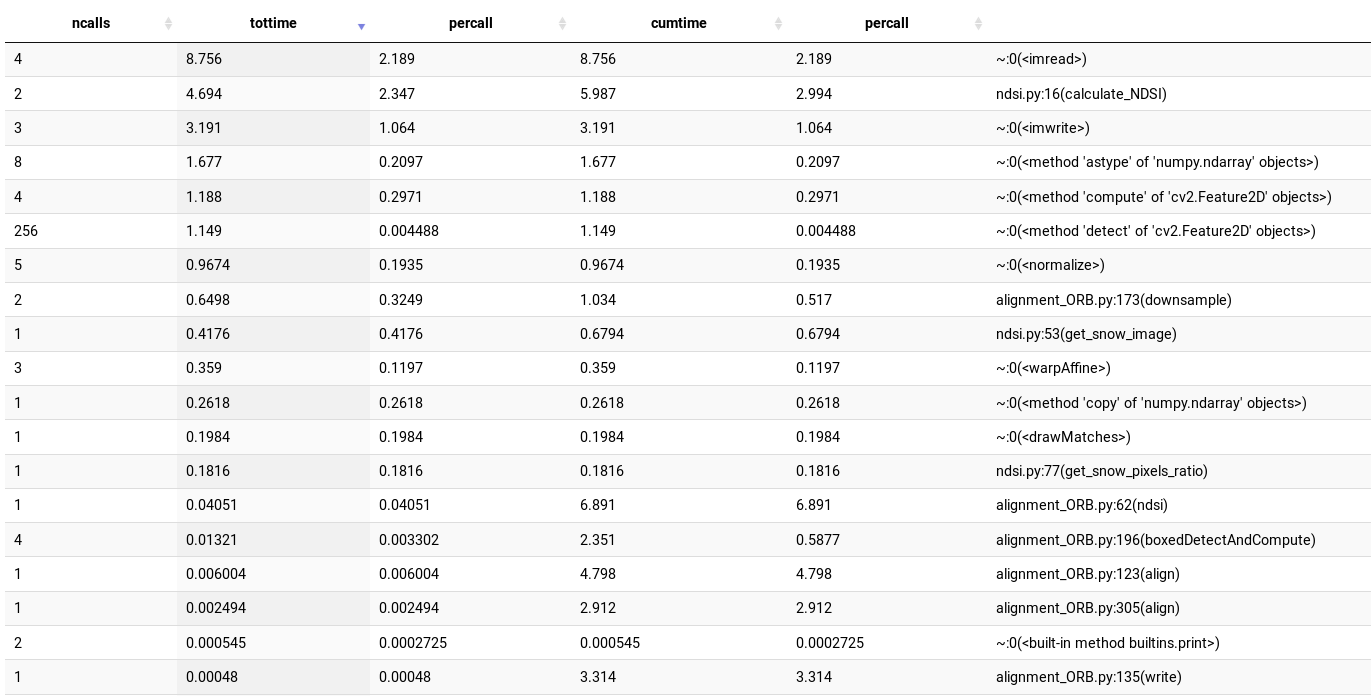
\includegraphics[scale=1]{profilebottom.png}
		\caption{Profile data on application run, detailed.}
		\label{fig:Profile bottom}
	\end{figure}
	.
	\newpage{}
	
	\chapter{Data set Structure}
	
	\section{Satellite Imagery}
	Satellite images are images of Earth or other planets collected by imaging satellites operated by governments and businesses around the world \cite{satellite_images}. The first collected images date from 1959, when the Explorer 6 was launched, followed by the Landsat program in 1972 which still functions to this date, holding the position of the largest program for image acquisition of Earth from space \cite{satellite_images}.
	%LANDSAT 8 SATELLITE
	\section{Landsat 8}
	The data used in this thesis is collected by the Landsat 8 Earth observing satellite, launched on 13 February 2013, as a collaboration between NASA and USGS \cite{temporal}. NASA took over the construction of the satellite, while USGS focused on maintaining it by calibration, generation of data scenes and storing them. The Landsat program goal is to collect and store 30 meters spatial resolution multispectral image data affording seasonal coverage of the global landmasses for a period of at least 5 years, while also ensuring that the data is consistent during this period, in terms of geometry, calibration, coverage characteristics, output product quality and data availability to ensure that studies over time can be done \cite{landsat_wiki}\cite{temporal}. The satellite products are free to use, stored in the Landsat Archive.
	\begin{figure}[h]
		\centering
		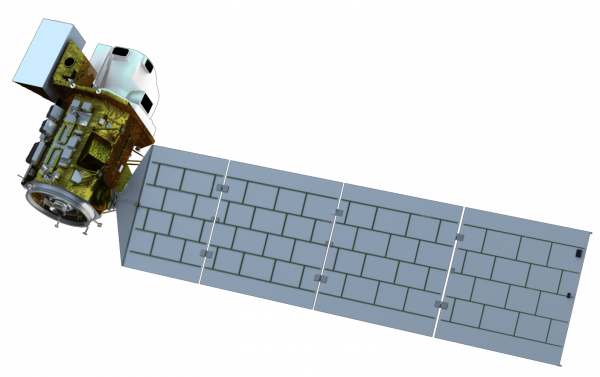
\includegraphics[scale=0.4]{landsat_8.png}
		\caption{Landsat 8 satellite \cite{landsat_8_image}.}
		\label{fig:Landsat8_satellite}
	\end{figure}
	
	\subsection{Worldwide Reference System}
	The Landsat data uses the WRS2 coordinate system, which uses path and row variables, which cover all the land surface of the Earth. The row equals the latitudinal center of a frame, while the path moves along the path and scans the land below \cite{wrs2}. The combination of the two creates the center of a Landsat scene which is identified as unique based on this notation. (more on Landsat naming convention). The rows and paths of the world land coverage are shown below:
	\begin{figure}[h]
		\centering
		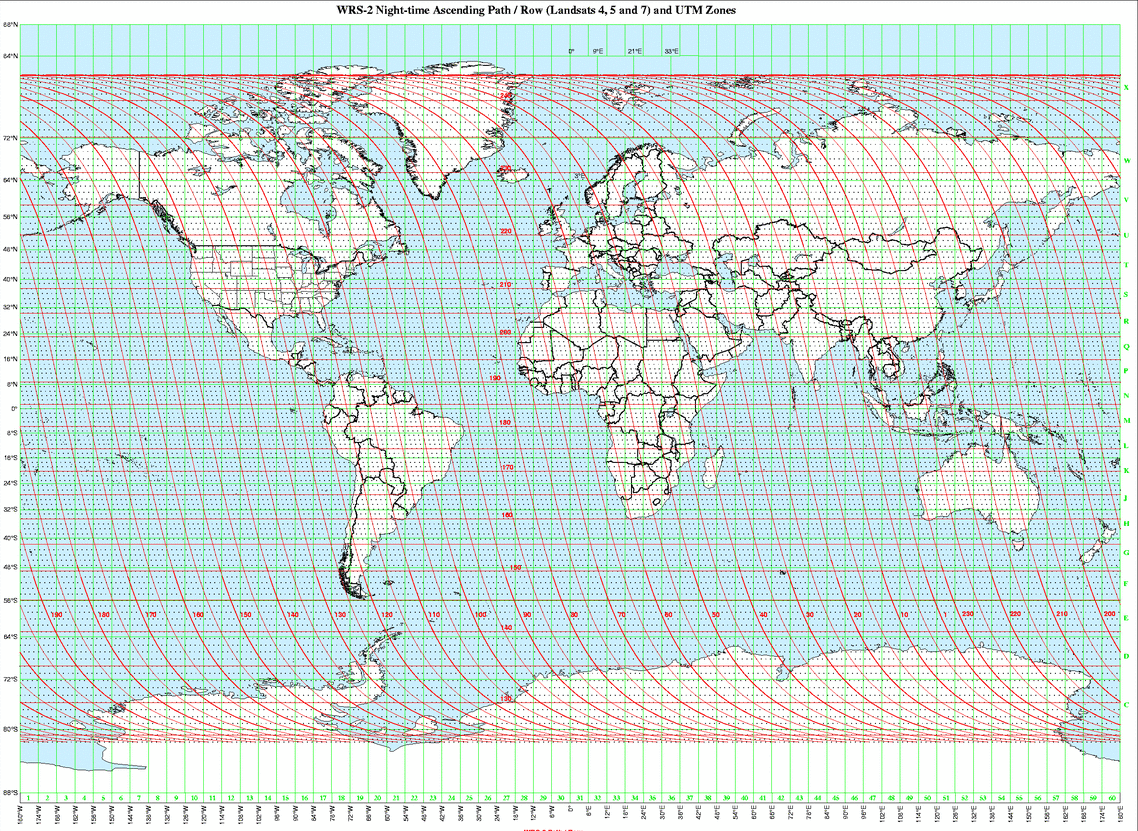
\includegraphics[scale=1]{worldwide_reference.png}
		\caption{Worldwide Reference System land coverage \cite{wrs2}.}
		\label{fig:wrs2_path_row}
	\end{figure}
	
	The collection used for image analysis in the thesis is Landsat Collection 1 Level-1.
	Landsat 8 is the latest and most technologically advanced satellite in the Landsat program. It has been equipped with two sensors, OLI and TIRS.
	
	\subsection{Operational Land Imager (OLI)}
	The OLI sensor is a push-broom sensor with a four-mirror telescope and a 12-bit quantization. It collects data from the visible, near infrared and short wave infrared spectral bands, as well as panchromatic band \cite{wavelength}. The sensor can capture areas of 185 kilometers \cite{oli}, and it is constructed such that the resolution is good enough to distinguish objects like cities, farms, small islands and other objects which were not seen as detailed in the previous Landsat satellites, due to the different spatial resolution, as seen in the below chart (Figure 2.2):
	\begin{figure}[h!]
		\centering
		\includegraphics[scale=2]{oli_wavelight_7_vs_8.jpg}
		\caption{OLI wavelength comparison between Landsat 7 and 8 \cite{wavelength}.}
		\label{fig:wavelength_comparison}
	\end{figure}
	
	\subsection{Thermal Infrared Sensor (TIRS)}
	The TIRS works by detecting the wavelengths of light emitted by the planet, which have a varying intensity depending on the temperature of its surface. The mechanics of measuring the wavelengths use quantum physics, and are stored in two thermal bands (band 10 and band 11) \cite{tirs}. Since in the thesis only band 3 and 6 will be used for processing, the thermal bands 10 and 11 will not be necessary.
	
	\section{Resolutions}
	When dealing with satellite image data, the resolution has an important role in its value. There are four types of resolutions: \textit{radiometric, temporal, spectral, spatial}.
	\paragraph{Radiometric resolution}
	The radiometric resolution represents the ability of a digital sensor to distinguish between grey-scale values \cite{radiometric}. The collected images are either 8-bit, 11-bit, 12-bit or 16-bit, depending on the sensor. Having large values of bit depth increase the number of features an image has and the ability to spot them. 
	
	\paragraph{Temporal resolution}
	The temporal resolution represents the frames of image collection, measured in temporal attributes such as hours or days. The Landsat 8 observing satellite captures an average of 700 images per day \cite{temporal}, and a 16-day repeat circle, referenced to the Worldwide Reference System-2 (WRS2) \cite{landsat_satellite}.
	\vskip 0.2cm
	
	\paragraph{Spectral resolution}
	The spectral resolution represents the number of spectral bands in which the sensor can collect reflected radiance \cite{spectral} \cite{band_combination}.
	The data collected for the elaboration of this thesis is from the Landsat 8 satellite, which has a multispectral resolution, consisting of 11 bands, as described below:
	\begin{figure}[ht]
		\centering
		\includegraphics{landsat_8_bands.jpg}
		\caption{Landsat 8 spectral resolution \cite{landsat_resolution}.}
		\label{fig:landsat8_bands}
	\end{figure}
	\vskip 0.2cm
	
	\paragraph{Spacial resolution}
	The spatial resolution is evaluated by how much of the image a pixel represents, which gives its detail. An approximate Landsat 8 scene size is 170 km north-south by 183 km east-west \cite{oli}. The Landsat 8 satellite is equipped with two sensors, the Operational Land Imager (OLI) and Thermal Infrared Sensor (TIRS). These two sensors provide coverage at a spatial resolution of \cite{wavelength}:
	\begin{itemize}
		\item 15 meters: panchromatic;
		\item 30 meters: visible, NIR, SWIR;
		\item 100 meters: thermal.
	\end{itemize}

	\section{Data set Collection}
	% COLLECTION PROCESS
	\subsection{Collection process}
	The satellite collects the images by moving across the path and scanning the land under it, while the instrument signals are transmitted to Earth and correlated with telemetry ephemeris data to form individual framed images. During this process, the continuous data are segmented into individual frames of data which represent the scenes \cite{wrs2}. 
	\subsection{Landsat Image Collection}
	The image collection used in this thesis is the Landsat Collection 1 Level-1, which is generated by the OLI and TIRS sensors of the Landsat 8 satellite. The implementation of the Collection represents a significant change in the management of the Landsat Archive by ensuring consistent quality through time and across instruments, along with additional changes like meta data and file names \cite{collection_1}.
	\paragraph{Collection 1 Tier 1}
	The aim of the collection tiers is to ensure that the data gathered from the satellite is of good quality and easy identification, such that it can be used for time-series pixel-analysis \cite{collection_1}. The Landsat8 scenes are processed and available for download in an average of 5-6 hours; after being reprocessed with definite ephemeris, updated bumper mode parameters and refined TIRS parameters, the products are transitioned to Tier 1 or 2, a process which usually takes between 14 and 26 days \cite{collection_1}. The scenes are divided into Tier 1 and Tier 2 based on the quality for the product. The images which are used in this thesis are Tier 1 images, and were chosen because of the higher quality and noted to be time-series analysis safe. 
	
	% Data set IMAGES
	\section{Data set Images}
	\subsection{Landsat 8 Bands}
	The Landsat 8 bands are TIFF images with a resolution between 7000 and 8000 pixels, with 1 pixel representing 30 meters. One scene covers about 210 km and it is updated at every 16 days. The bit-depth of the images is 16 and are captured in gray-scale. For the elaboration of the thesis, only the third and sixth bands will be used in the calculation of the Normalized Difference Snow Index, so they will be detailed below with examples of images for each.
	% GREEN BAND
	\subsection{Green Band}
	Green band image specifications:
	\begin{table} [H]
		\center
		\begin{tabular} {|  l | L{10cm} |}
			\hline
			Wave-length & 0.53- 0.59 micrometers \\ [0.2ex]
			\hline
			Spacial Resolution & 30 meters \\ [0.2ex]
			\hline
			Depth & 16-bit \\ [0.2ex]
			\hline
			Resolution & aproximately 7500x7500 pixels \\ [0.2ex]
			\hline 
			Format & Gray-scale \\ [0.2ex]
			\hline
		\end{tabular}
		\caption{Green Band Specifications \cite{green_band, band_combination}.}
		\label{table:green_band_specifications}
	\end{table}
	Due to its wave-length, the green band is one of the three bands from the visible spectrum, along the blue and red band \cite{band_information}. The following image is an example of a green band taken from the AT4J143FA006 glacier:
	\begin{figure}[H]
		\centering
		
\includegraphics[scale=1]{LC81930272018108LGN00_B3.png}
		\caption{Landsat 8 Band 3 (Glacier (ID) AT4J143FA006 at (10.803, 47.007) coordinates.
			\cite{green_band}}
		\label{fig:band3}
	\end{figure}
	% SWIR1 BAND
	\subsection{SWIR1 (Infrared) Band}
	SWIR1 band image specifications:
	\begin{table} [H]
		\center
		\begin{tabular} {|  l | L{10cm} |}
			\hline
			Wave-length & 1.57 - 1.65 micrometers \\ [0.2ex]
			\hline
			Spacial Resolution & 30 meters \\ [0.2ex]
			\hline
			Depth & 16-bit \\ [0.2ex]
			\hline
			Resolution & aproximately 7500x7500 pixels \\ [0.2ex]
			\hline 
			Format & Gray-scale \\ [0.2ex]
			\hline
		\end{tabular}
		\caption{SWIR1 Band Specifications \cite{band_information, band_combination}.}
		\label{table:swir1_band_specifications}
	\end{table}
	The SWIR1 band covers one part of the shortwave infrared spectrum, invisible to the human eye. It enhances geology objects such as rocks and soils which look similar in other bands \cite{band_information}, making them visible and easy to analyse
	\begin{figure}[H]
		\centering
		
\includegraphics[scale=1]{LC81930272018108LGN00_B6.png}
		\caption{Landsat 8 Band 6 (Glacier (ID) AT4J143FA006 at (10.803, 47.007) coordinates. 
			\cite{swir1_band}}
		\label{fig:band6}
	\end{figure}

	
	\subsection{The Normalized-Difference Snow Index}
	% NORMALIZED DIFFERENCE SNOW INDEX
	The NDSI represents the normalized difference of the two described bands, the green band in the visible spectrum and the SWIR1 one in the shortwave infrared spectrum. By calculating the NDSI between the two bands, the result will \textbf{enhance snow in a Landsat scene}, due to snow's high reflectance in the visible spectrum (0.66 mm) and high absorption in the short-wave infrared one (1.6 mm) \cite{ndsi_1, ndsi_2}. The mapping is done by computing the following formula:
	\[ndsi = \frac{green - swir1}{green + swir1}    \cite{ndsi_2}\]
	% TABLE
	\begin{table} [H]
		\center
		\begin{tabular} {|  l | L{10cm} |}
			\hline
			ndsi & result which holds the normalized image \\ [0.2ex]
			\hline
			green & third band of the Landsat 8 satellite \\ [0.2ex]
			\hline
			swir1 & sixth band of the Landsat 8 satellite \\ [0.2ex]
			\hline
		\end{tabular}
		\caption{Normalized-Difference Snow Index variables.}
		\label{table:ndsi_table}
	\end{table}
	
	The NDSI is used at mapping the glaciers from the collected Landsat 8 images, so that the creating the data set consisting of snow pixels over total pixels is accurate. For \textbf{snow mapping}, the NDSI is applied on the two images with a \textbf{threshold of contrast} so the gray-scale will be just black and white, meaning glacier or no glacier pixel. This is done so that when processing the images on time-series, the values are easier to parse and predict. By applying the formula on the Figures 2.6 and 2.7 and a threshold of contrast of 0.5, the following result is created:
	\begin{figure}[H]
		\centering
		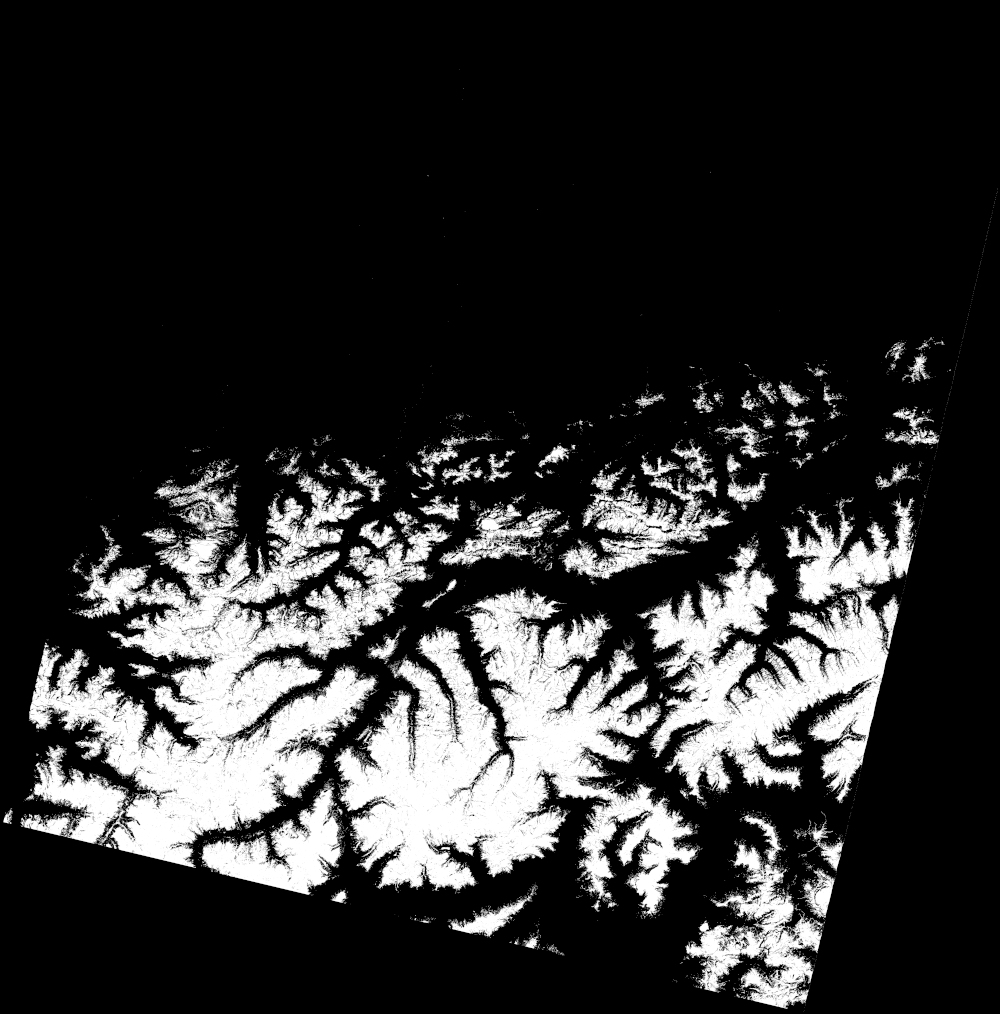
\includegraphics[scale=1]{result(2).png}
		\caption{NDSI and contrast between green and SWIR1 bands.}
		\label{fig:ndsi}
	\end{figure}
	
	\subsection{Landsat scene name convention}
	Each Landsat scene has an unique name which holds general information to analyze it at a high level without the need of processing or opening the image beforehand. The identifier for the Collection 1 Level 1 has the following general name:
	\begin{center}
		LXSPPPRRRYYYYDDDGSIVV \cite{landsat_scene_name}
	\end{center}
	\begin{itemize}
		\item \textbf{LSX}: The firs three letters describe what type of satellite and sensor were used;
		\item \textbf{PPPRRR}: The following six letters describe where the scene is located by the WRS2 path and row location
		\item \textbf{YYYYDDD}: The next seven letters represent when the scene was acquired, using the Julian calendar by counting the number of days passed starting January 1 \cite{landsat_scene_name};
		\item \textbf{GSIVV}: The last five letters describe how the data was received from its ground stations, which are data capture facilities to obtain transmitted satellite data \cite{landsat_scene_name}.
	\end{itemize}
	
	\section{Programming Environment: PyCharm} 
	The application of the thesis has been written in the PyCharm IDE, which is specialized in Python programming language. The IDE ensures clean code writing by analyzing it, code debugging implemented in the graphical user interface, safe testing by adding unit test support and supports revision control with systems like Git, which has been used for version control of the writing of the application. The IDE is cross-platform with Windows, mac OS and Linux \cite{pycharm}
	The environment has been chosen for the development of the application because it includes features such as code assistance, easy python code re-factoring and revision control with Git.
	
	%PYTHON
	\section{Python Programming Language}
	Python is an interpreted, high-level, general-purpose programming language, created by Guido van Rossum and first released in 1991 \cite{python} The goal of python is simplicity, so that the programmers can achieve logical constructs in their projects at whichever scale, supporting this by being a high-level language, having an implicit garbage collector which takes care of the memory and granting access to many open-source libraries which can be used to as a puzzle to create something.
	Due to its flexibility and simplicity, Python has been chosen as the main and only language the application is written in. 
	
	%GIT
	\section{Git}
	Git is a free, open-source distributed version-control system for tracking changes in the source code during software development, created by Linus Torvalds in 2005 \cite{git_general}\cite{git_definition}. Its goal is to ensure a good work-flow during the creation of a project by keeping track of any chances in all the files of the project during its development, as well as fast and easy usage, data integrity\cite{git_general} \cite{git_linus_1} and support for distributed, non-linear work-flows \cite{git_linus_2} \cite{git_general}. \\
	Git works by flagging a directory as a repository of the project, therefore keeping track of each file and its history in that location, independent of network access or a central server \cite{git_general}. It, therefore, creates a more structured project development, making it easier to implement different features without breaking the stable version, go back and change things which were not supposed to be released, maintain the released versions and fix bugs. 
	Using Git to keep version control of the application has proven very efficient and time-saving in most situations, ensuring easy fixes, trace-backing, scaling and feature adding. 
	
	\section{Libraries}
	% GDAL
	\subsection{Geospatial Data Abstraction Library (GDAL)}
	GDAL is an open-source translator library for raster and vector geo-spatial data formats \cite{gdal_general}, presenting a single abstract data model to the calling application for all supported formats, while also providing strong command line interface utilities for data translation and processing \cite{gdal_1}. In the application, GDAL is used as an image reading tool as an alternative to the OpenCV one. 
	
	% NUMPY
	\subsection{NumPy}
	NumPy is the fundamental package for scientific computing with Python, containing powerful tools for N-dimensional arrays handling \cite{numpy_definition} such as optimized matrix algebra, easy conversion from images to matrices for pixel-level algebra, which is used in the application for processing the TIFF data as matrices rather than images. NumPy was chosen as the mathematical handler of the application for its capabilities of handling big data files by using high-level mathematical functions to ensure a trustworthy file process, therefore ensuring a better performance \cite{numpy_wiki}.
	
	% OPENCV
	\subsection{OpenCV}
	OpenCV is a library of programming functions mainly aimed at real-time computer vision, supporting deep-learning. The initial goal of OpenCV was to handle Intel Research intensive CPU-applications by providing open and optimized code for basic vision infrastructure, and common infrastructure so developers could build easier to read and transferable code \cite{opencv_wiki}. The library was used in the application for image alignment and display working with the TIFF images collected from the satellite, as well as image alignment and difference and movement image creation.
	
	\subsection{sat-search}
	Sat-search is a Python 3 library and a command line tool for discovering and downloading publicly available satellite imagery using a conformant API \cite{sat-search}. It is used in our application for searching and downloading Landsat 8 images from the archive.
	
	\newpage{}
	
	
	
	
	\chapter{The application}
	
	
	\section{Functional description} 
	% SATELLITE DATA COLLECTIONS % 
	\subsection{Satellite Data Set Building}
	\subsubsection{Earth Explorer}
	An accurate analysis on glacier change in time needs a large enough data set of images to work with. The Landsat 8 images are free to use and in huge numbers, but they are not that easy to access in bulk. An example of an user friendly tool to access and view the images is \textbf{Earth Explorer} \cite{earth_explorer_1}, which is used for searching catalogs of satellite and aerial imagery with the option of downloading data over chronological time-lines, wide range of specifying search criteria and a long list of satellite and aerial imagery to choose from \cite{earth_explorer_2}. The only downside of the tool is that searching and downloading data sets takes quite a lot of time, since its parameters need to be manually set, and for each found entry, the user must choose what to download individually, then use another application to launch the bulk download and finally have access to the local data. Overall, the process of collecting a qualitative and large enough data set using Earth Explorer is very time consuming, and is desirable only if the user wants to view the samples on the map before actually downloading them. the An example of the Earth Explorer tool is shown below, with searching of images from path 67 row 18, from Landsat 8 Collection 1 Level 1.
	\begin{figure}[H]
		\centering
		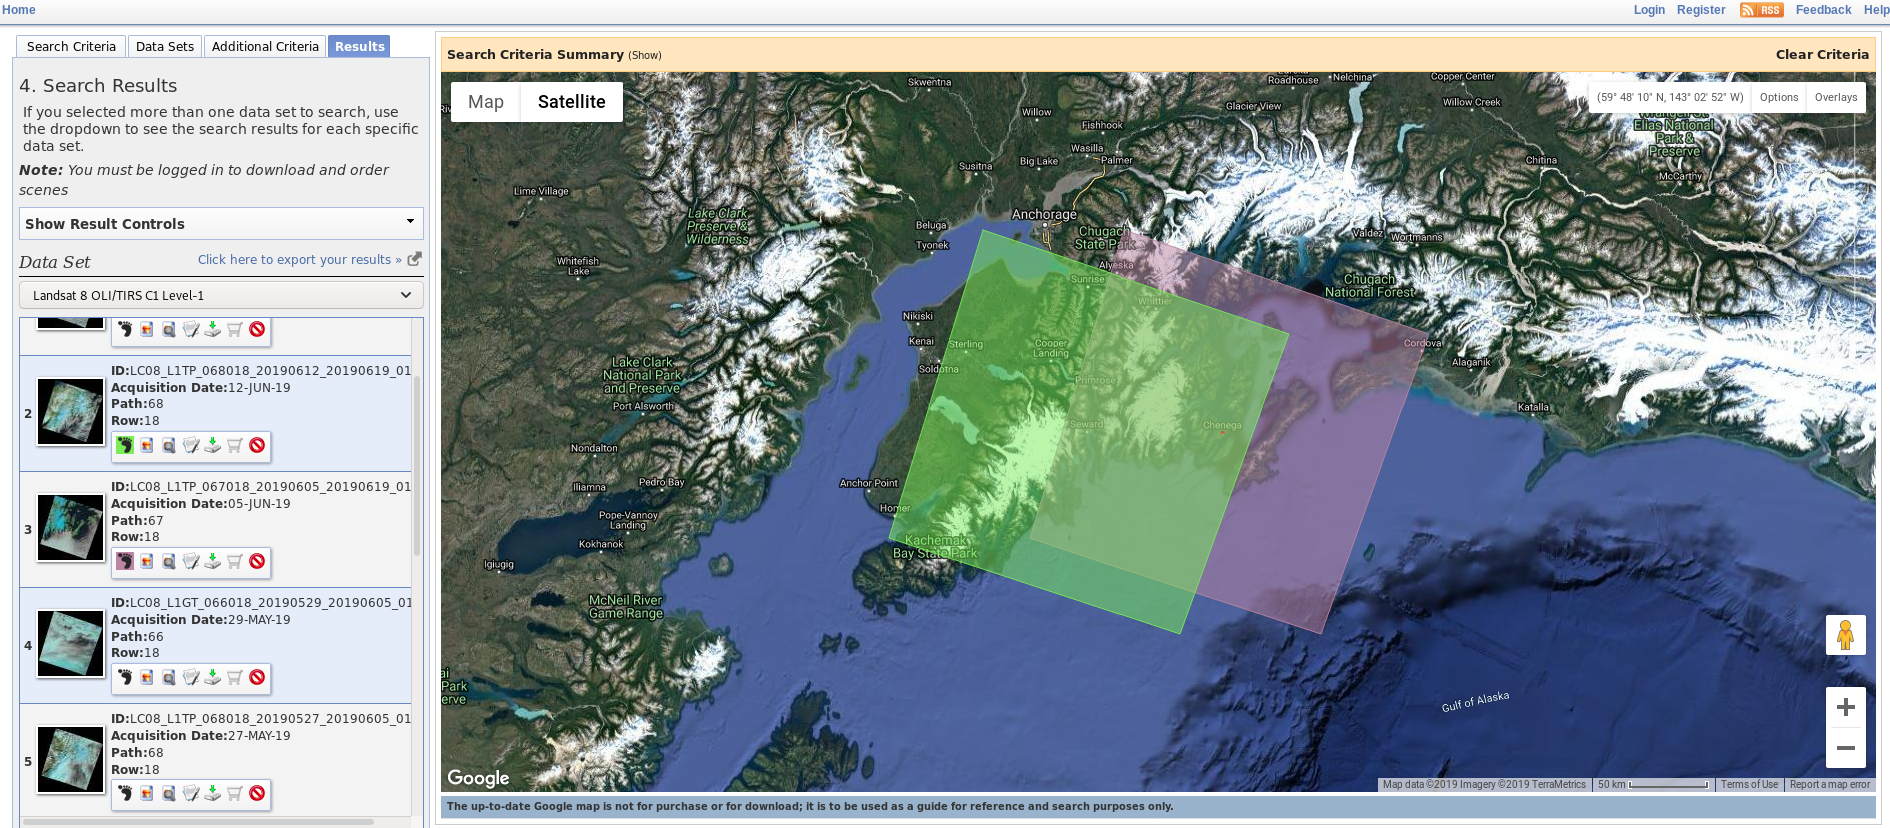
\includegraphics[scale=0.85]{earth_explorerpng.png}
		\caption{Earth Explorer \cite{earth_explorer_1}.}
		\label{fig:Earth_Explorer}
	\end{figure}
	\vfill 
	As a solution to make sure that creating the data set when no visualization beforehand is needed is as trivial as possible was implementing searching and downloading of Landsat 8 scenes as a feature of our application with a simple command line interface call, as shown below:

	When dealing with collecting of Landsat 8 data, there are x problems to take in consideration:
	\begin{itemize}
		\item Where is the data collected from?
		\item How are the glacier scenes found?
		\item Where are they downloaded to?
	\end{itemize}
	\subsubsection{Where is the data collected from?}
	Landsat scenes are available to download from the Landsat Archive, which stores all the captured scenes since the Landsat 8 satellite was launched. All the information about the data is easy to access by filling in parameters such as path and row variables, specific to Landsat, cloud coverage, date of gather, coordinates and many more. The possibility to narrow or widen the area of search are huge given that all these parameters can be combined so a desirable set is achieved, then downloaded. \textbf{USGS Landsat Global Archive} contains the information about how they are structured and where they are exactly found \cite{usgs_landsat_archive}.
	
	% HOW 
	\subsubsection{How are the glacier scenes found?}
	In order to be able to download only necessary data from the Landsat Archive, information about where exactly the glaciers are located is crucial to have. In order to simplify the process of finding information about coordinates of glaciers around the globe, we used instead the \textbf{World Glacier Inventory} \cite{world_glacier_inventory}, which contains the coordinates of over a \textbf{130.000 glaciers} around the globe. The CSV file containing their id's and coordinates is included in the application in order to facilitate the searching and giving the option to achieve results as fast as possible, without also worrying about building a suitable data set. If the user wants to create their own data set instead, there are two more options provided by the World Glacier Inventory team:
	\begin{itemize}
		\item Search Inventory interface;
		\item Extract Selected Regions interface.
	\end{itemize}
	
	% SEARCH INVENTORY INTERFACE
	
	\paragraph{Search Inventory interface}
	Search Inventory interface is a tool provided by the National Snow and Ice Data center (NSIDC) \cite{world_glacier_inventory} which enables searching of glacier items for inspection by parameters such as glacier: name, number, coordinates, altitude, size and length;

	\begin{figure}[H]
		\centering
		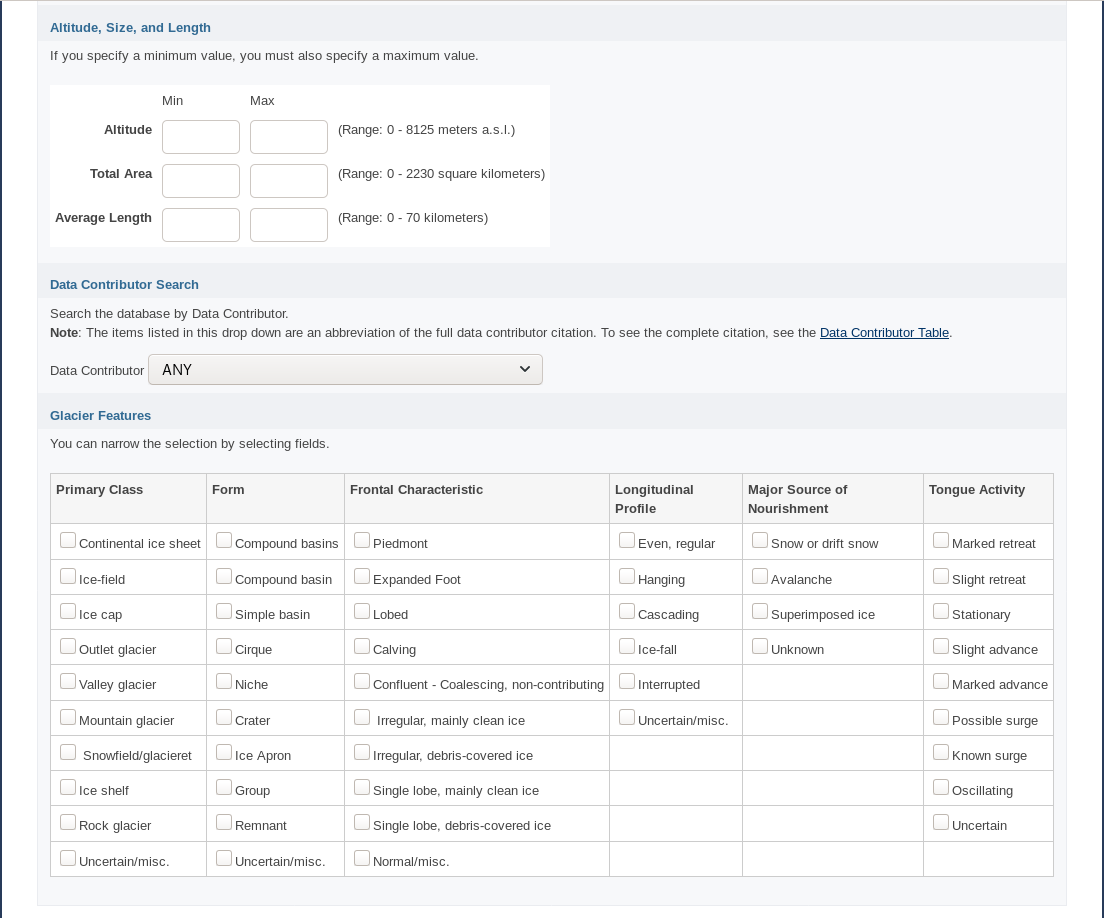
\includegraphics[scale=1]{nsidc_search.png}
		\caption{Search Inventory interface (NSIDC) \cite{nsidc_1}.}
		\label{fig:NSIDC_search}
	\end{figure}
	
	% EXTRACT
	\paragraph{Extract Selected Regions interface}
	The third option is to search for glacier based on their region, such that in case the user wants information based only on location, a suitable data set can be easily created rather than searching each item by hand and keeping only the ones from the desired region. An example of the search web interface is displayed below:
	\begin{figure}[H]
		\centering
		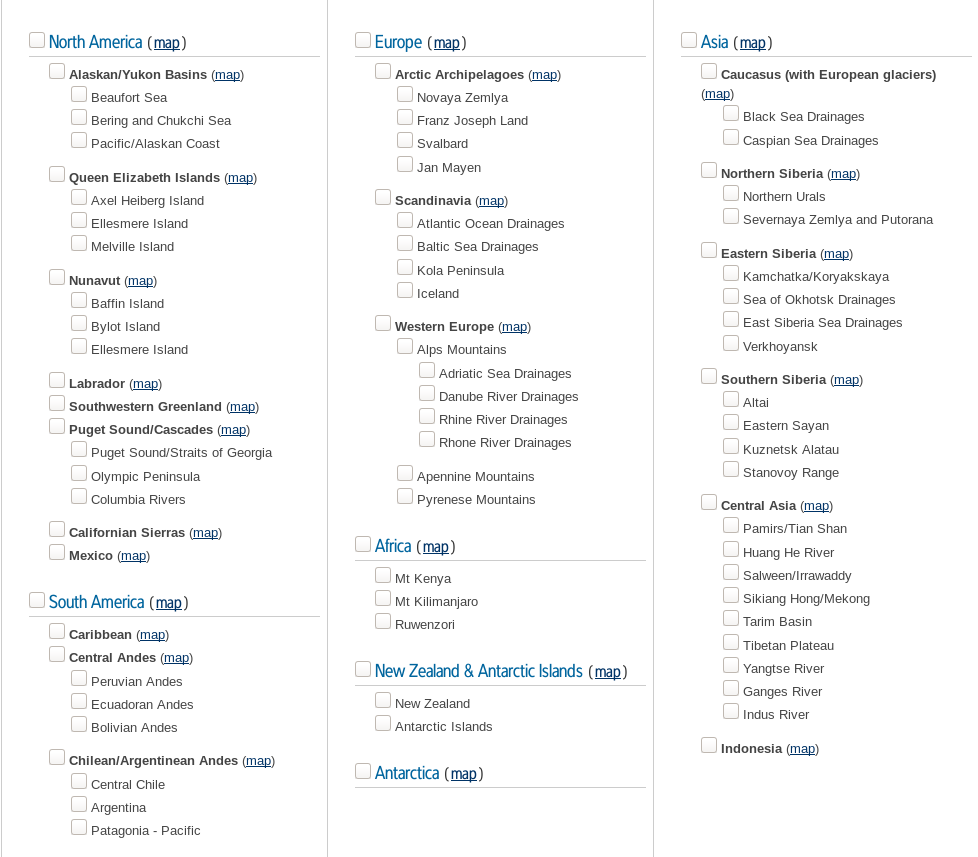
\includegraphics[scale=1.7]{ndsic_2.png}
		\caption{Extract Selected Regions interface (NSIDC) \cite{nsidc_2}.}
		\label{fig:NSIDC_extract}
	\end{figure}
	By choosing exact features from the searching tool, a smaller and more specialized data set is created in order to conduct a focused research.
	
	\subsubsection{Where are they downloaded to?}
	After the data set formed of Landsat 8 scenes has been built, the CSV containing the scenes information is used in order to begin the download of the selected files. In order to make the application as simple as possible from the user point of view, the selected items will be downloaded to a location of their choice on their computers. The folders will be structured based on the glacier's id, their paths and rows and the files which represent the results of the processing. A example of the folder structure for downloading is presented below:
	\begin{figure}[H]
		\centering
		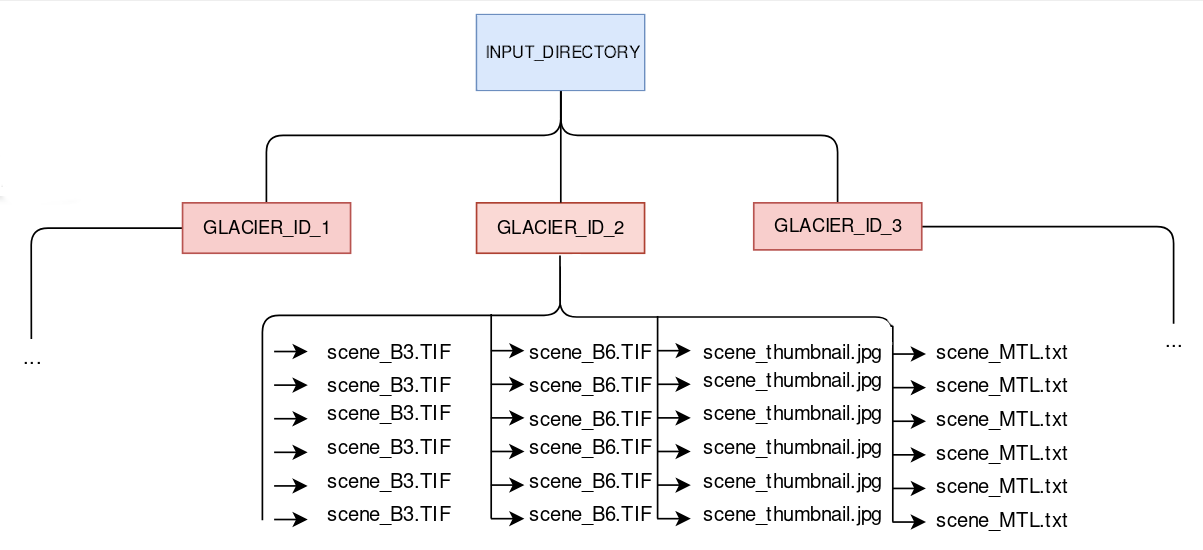
\includegraphics[scale=1.4]{download_folderhierarchy.png}
		\caption{Download folder hierarchy.}
		\label{fig:download_folders}
	\end{figure}
	
	\subsection{Data Set Information Extraction}
	In order to process the gathered Landsat 8 scenes, we will use the information provided by the meta-data file downloaded with each scene, as well as the scene's name which is formed by the Landsat 8 convention, detailed in the section Data set Images, Landsat scene name convention. With the information extracted from these sources, we can get to the prepossessing stage of the application.
	
	\subsubsection{Scene Metadata (MTL)}
	Each Landsat 8 scene comes with a meta data file containing useful information about the package, such as: \textbf{scene ID, output format, WRS path and row, date of acquiring, capture time, coordinates, bands of scene and many more.} There are \textbf{approximately 150 variables describing the scene}, which makes it an useful file to have in order to extract information when necessary. Below is shown an example of a portion of the MTL file for a scene:
	\begin{figure}[H]
		\centering
		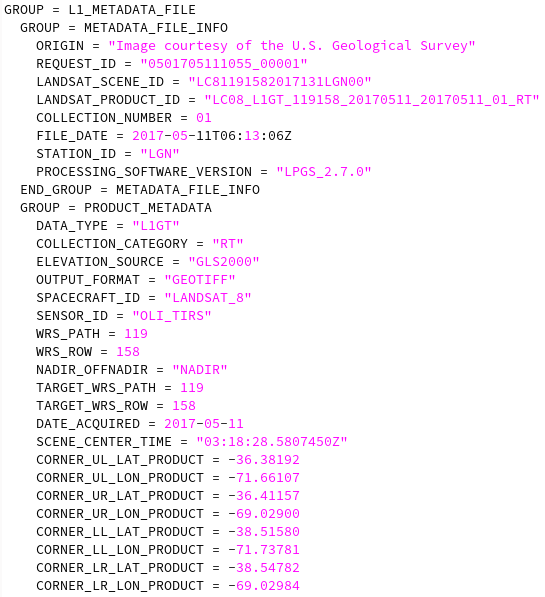
\includegraphics[scale=2]{metadata_example.png}
		\caption{Metadata file.}
		\label{fig:metadata_file}
	\end{figure}
	
	\section{Pre-processing}
	The pre-processing phase of the application implies traversing the directories which contains glaciers and build the folder structure to hold the results of the processing of the data set. Each glacier will have its own directory, formed of path and rows directory for all its pairs. The path and row directories will contain the results of the processing, the aligned NDSI images, as well as a csv file with information about the results of the processing, which will be described in 
	The folder splitting hierarchy is designed as follow:
	\begin{figure}[H]
		\centering
		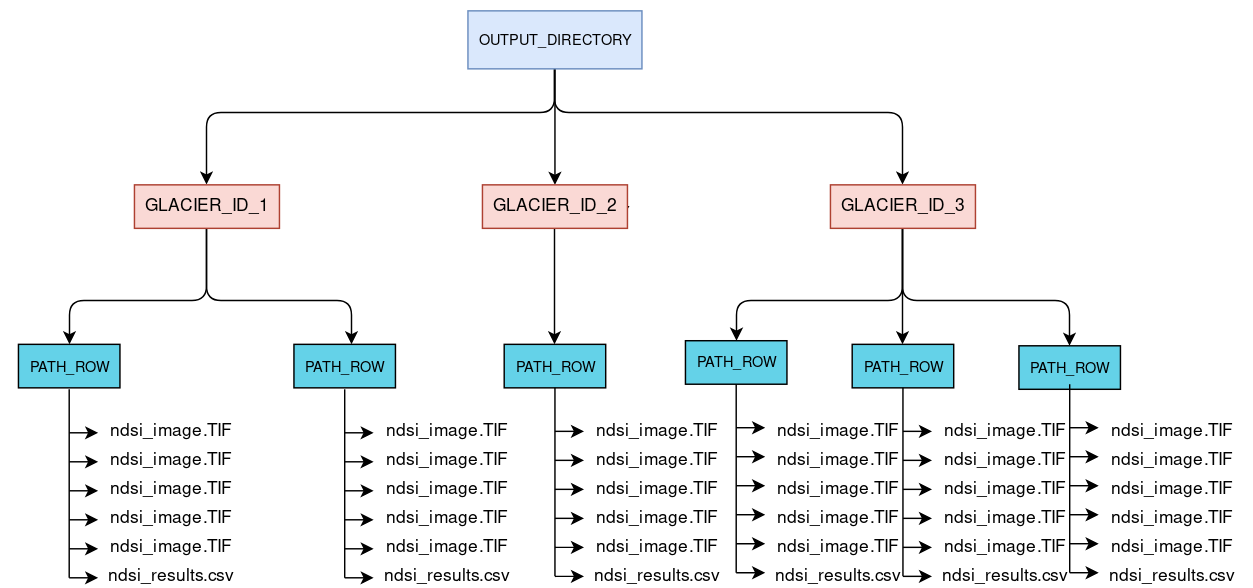
\includegraphics[scale=1.5]{process_folder_diagram.png}
		\caption{Output folder hierarchy.}
		\label{fig:output_folder_hierarchy}
	\end{figure}

  	% PROCESSING % 
  	\section{Processing}
  	In order to achieve a \textbf{time series forecast on snow coverage}, processing of the images is necessary. After the data set has been built, the information extracted and the pre-processing done, the paired images (by green and SWIR1 bands) will be processed with the following actions:
  	\textbf{
  		\begin{itemize}
  			\item Normalized Difference Snow Index (NDSI);
  			\item Alignment;
  			\item Object appearance and disappearance detection; 
  			\item Object movement flow.
  		\end{itemize}
  	}
  	
  	% NDSI build
  	\subsection{The Normalized-Difference Snow Index}
  	% NORMALIZED DIFFERENCE SNOW INDEX
  	The NDSI represents the normalized difference of the two described bands, the green band in the visible spectrum and the SWIR1 one in the shortwave infrared spectrum. By calculating the NDSI between the two bands, the result will enhance snow in a Landsat scene, due to snow's high reflectance in the visible spectrum (0.66 mm) and high absorption in the short-wave infrared one (1.6 mm) \cite{ndsi_1, ndsi_2}. The mapping is done by computing the following formula:
  	\[ndsi = \frac{green - swir1}{green + swir1}    \cite{ndsi_2}\]
  	
  	The NDSI is used at mapping the glaciers from the collected Landsat 8 images, in order to enhance them and make it easier to observe, analyses, apply image alignment based on their features and predict their movements based on pixel-analysis. For snow mapping, the NDSI is applied on the two images with a threshold of contrast so the gray-scale will be just black and white, meaning glacier or no glacier pixel. This is done so that when processing the images on time-series, the values are easier to parse and predict. By applying the formula on the Figures 2.6 and 2.7 and a threshold of contrast of 13000, the following result is created:
  	\begin{figure}[H]
  		\centering
  		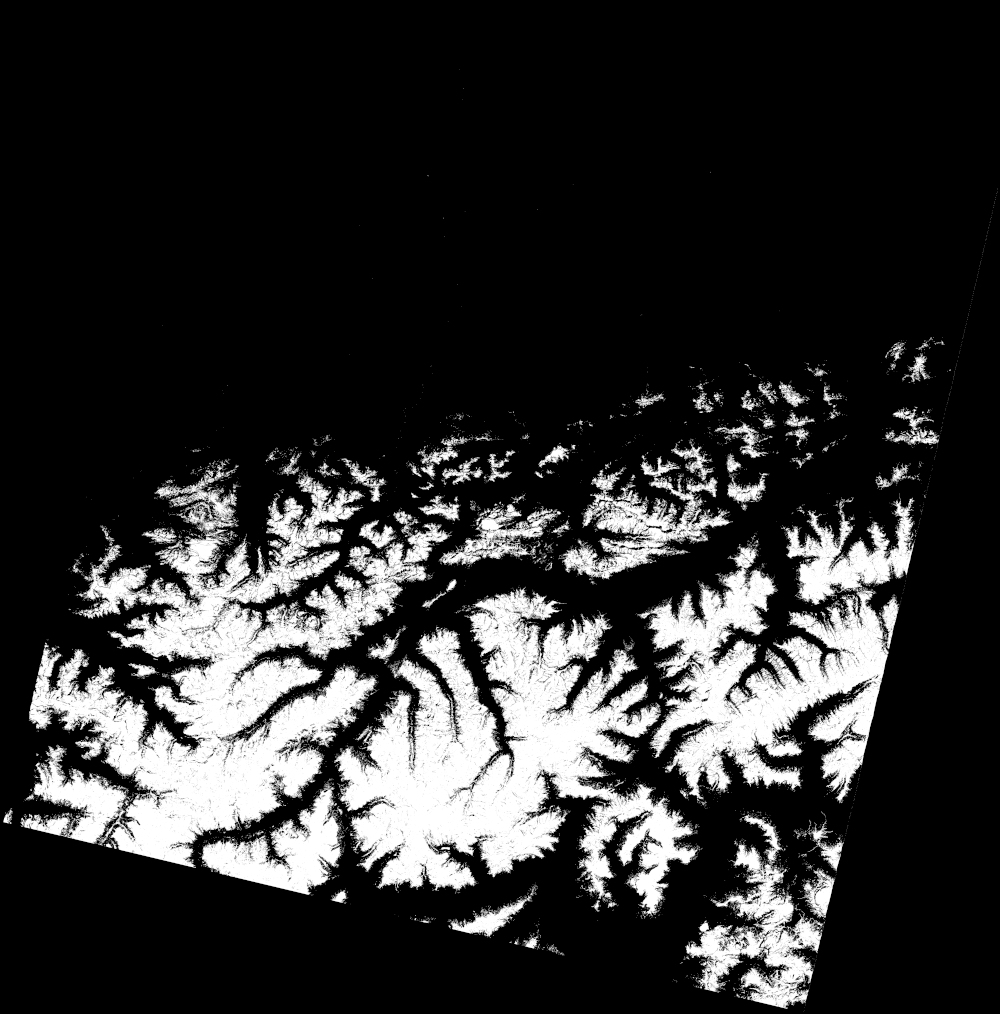
\includegraphics[scale=1]{result(2).png}
  		\caption{NDSI and contrast between green and SWIR1 bands.}
  		\label{fig:ndsi}
  	\end{figure}
  	
  	% ALIGNMENT 
  	\subsection{Image Alignment}
  	As a part of creating a forecast on a data set of images, alignment between them is necessary, due to pixel discrepancy from image to image. The difference is created by Landsat's trajectory when orbiting the Earth, which is not precise, therefore, not always passing on the same trajectory so the images are aligned to pixel level. Below will be exemplified the discrepancy between two green bands from two different scenes form the same path, row and glacier:
  	
  	% UNALIGNED
  	
  	\begin{figure}[H]
  		\minipage{0.32\textwidth}
  		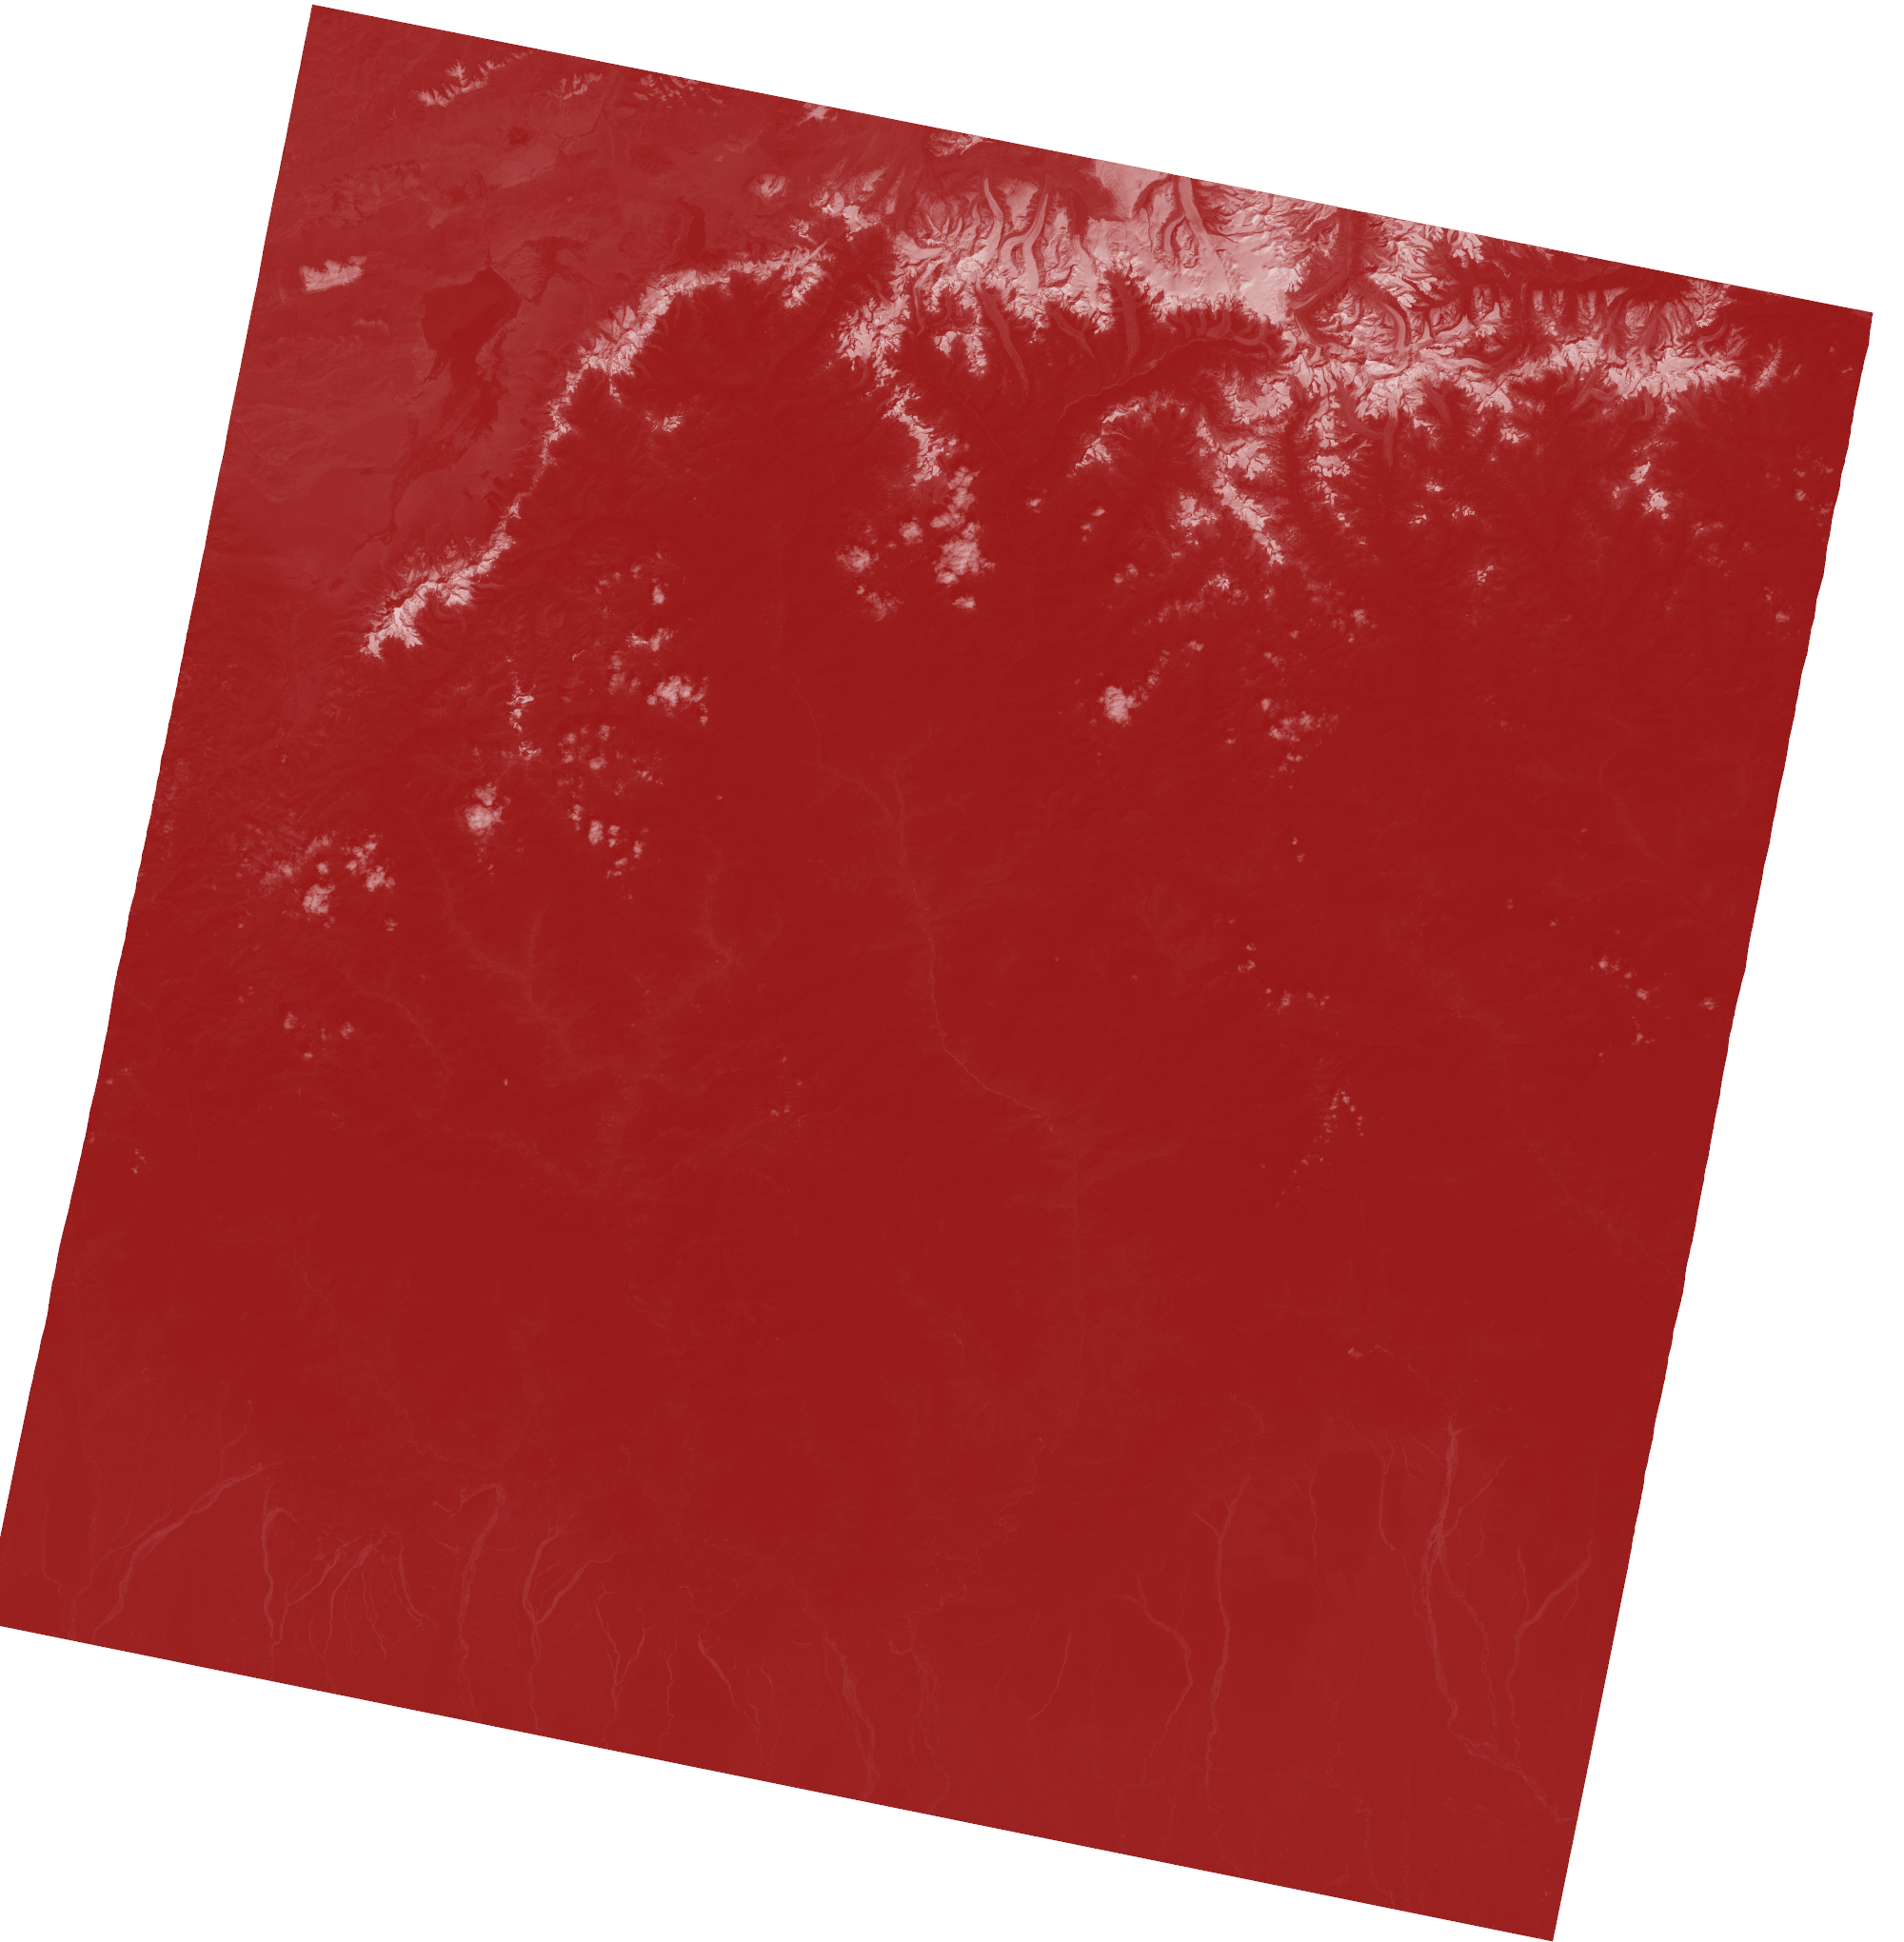
\includegraphics[width=\linewidth]{red_big_unaligned.png}
  		\endminipage\hfill
  		\minipage{0.32\textwidth}
  		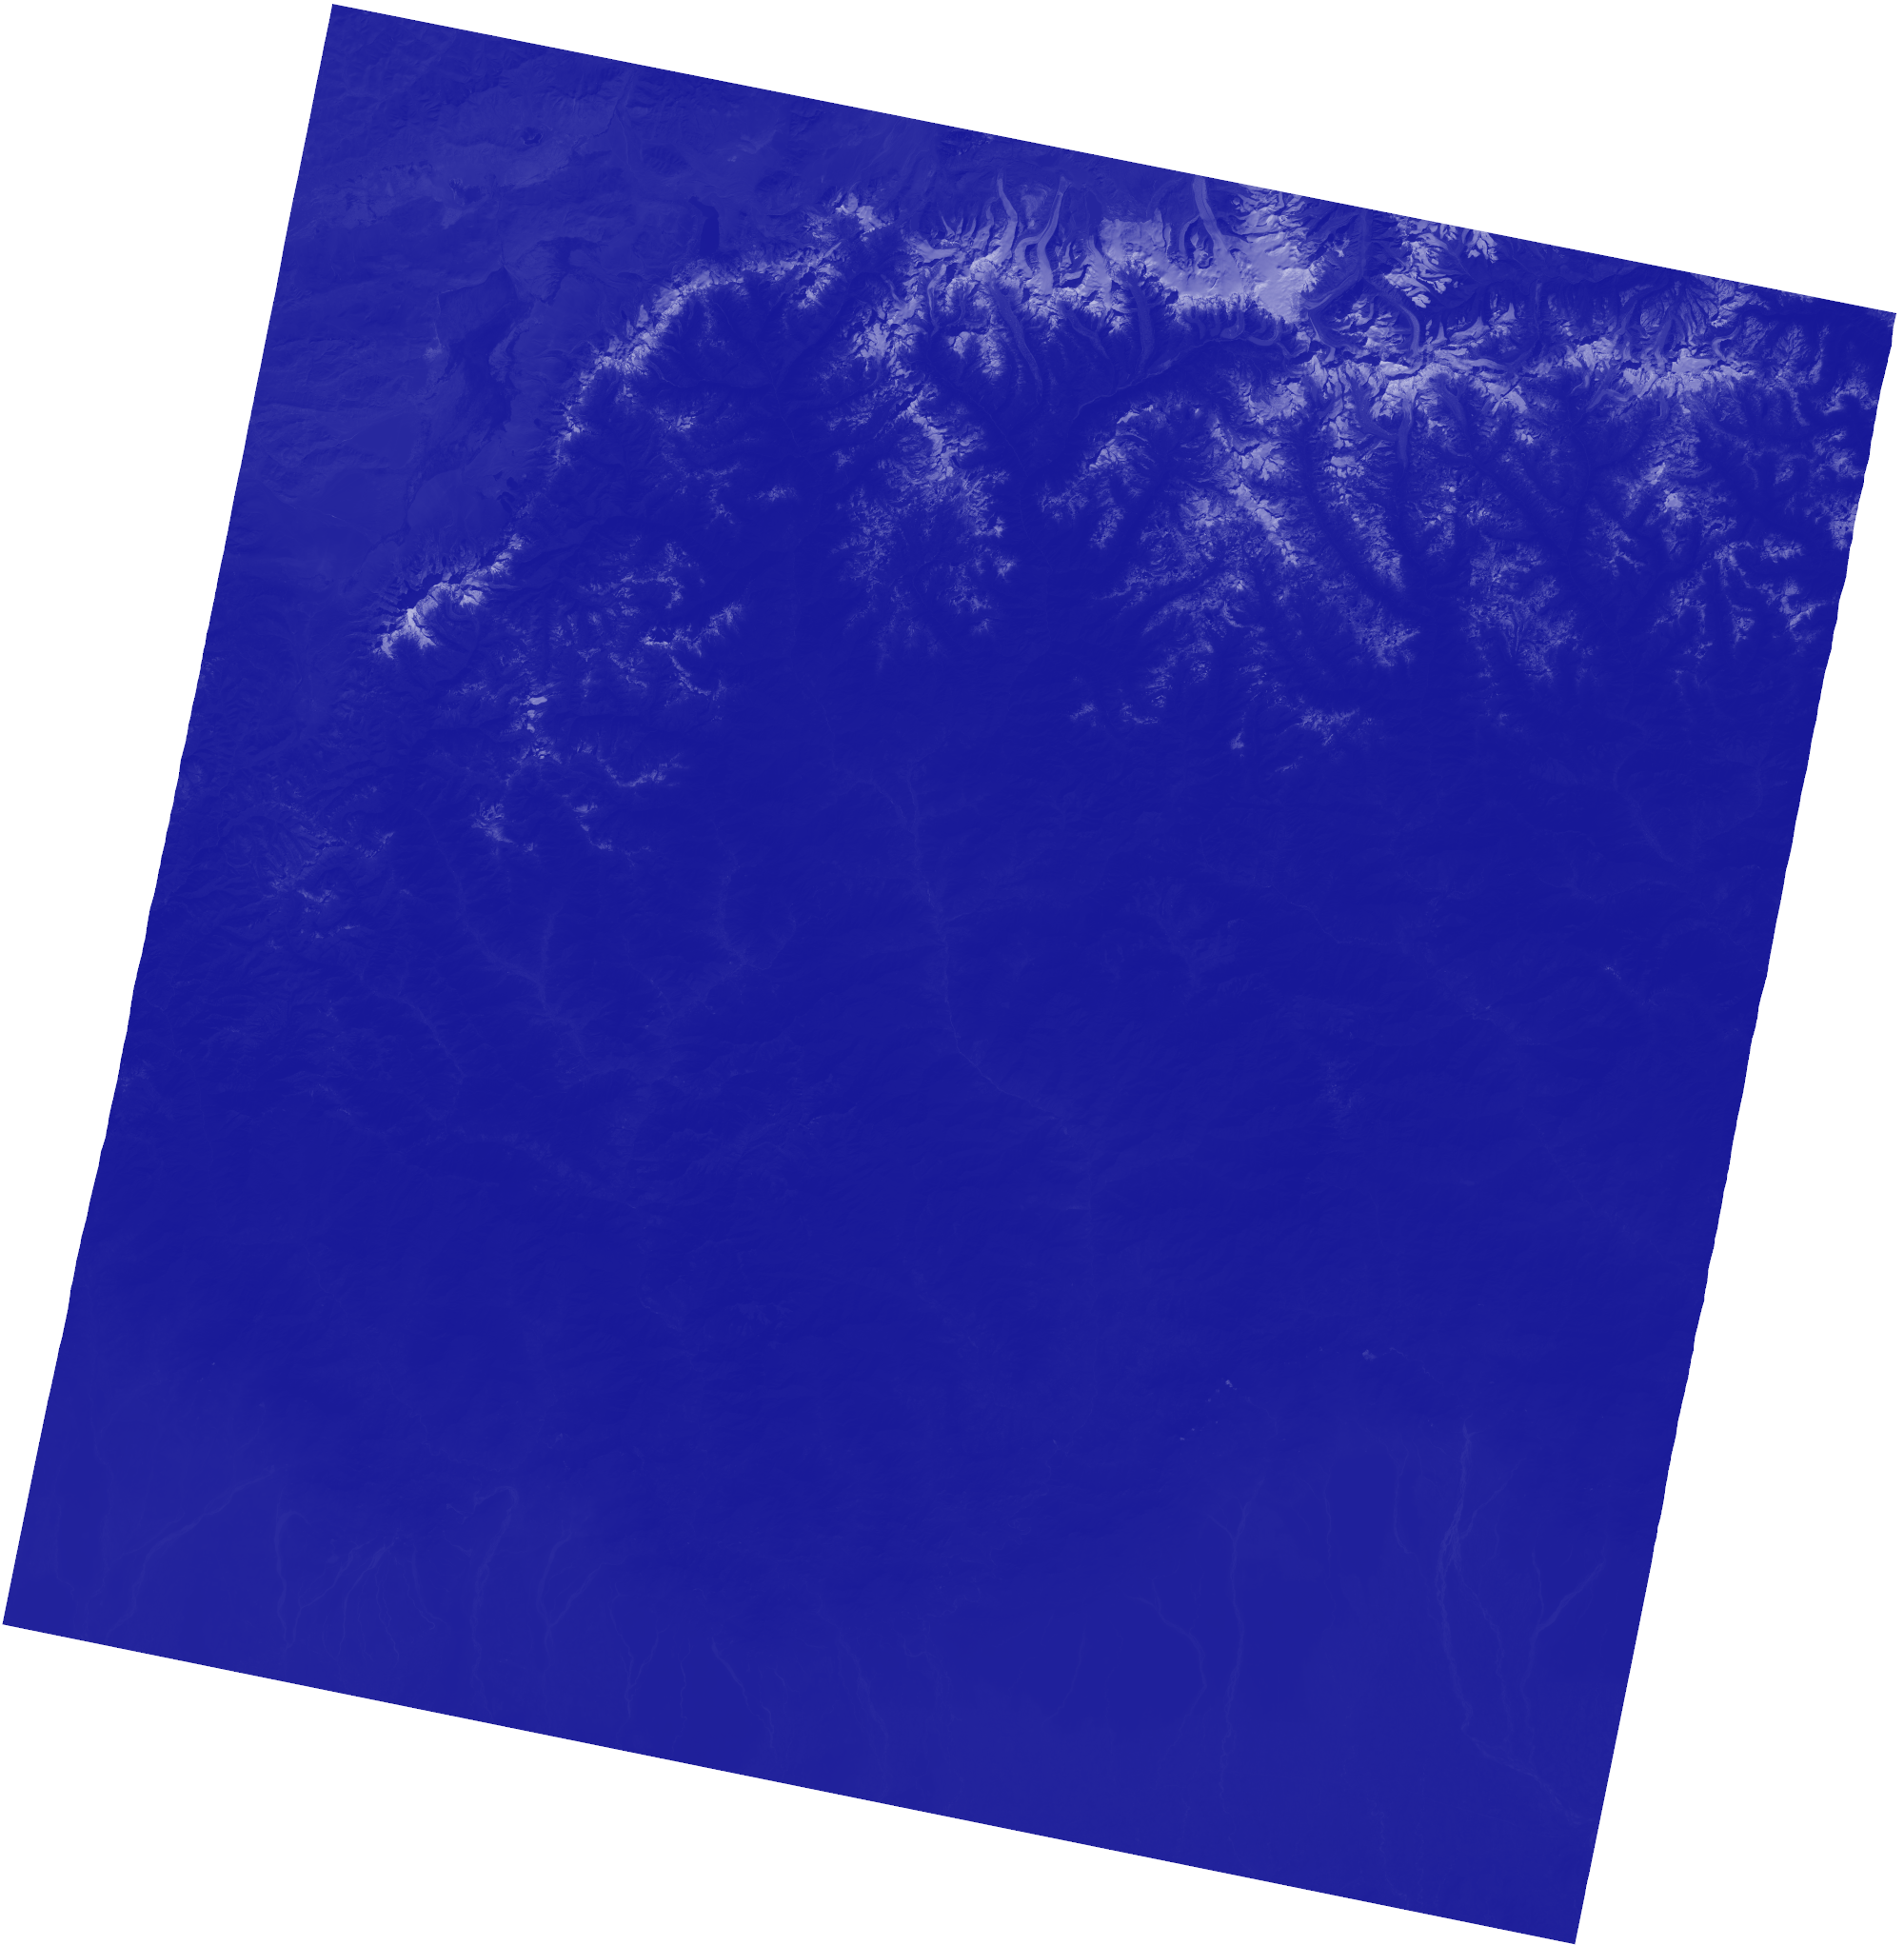
\includegraphics[width=\linewidth]{blue_big_unaligned.png}
  		\endminipage\hfill
  		\minipage{0.32\textwidth}%
  		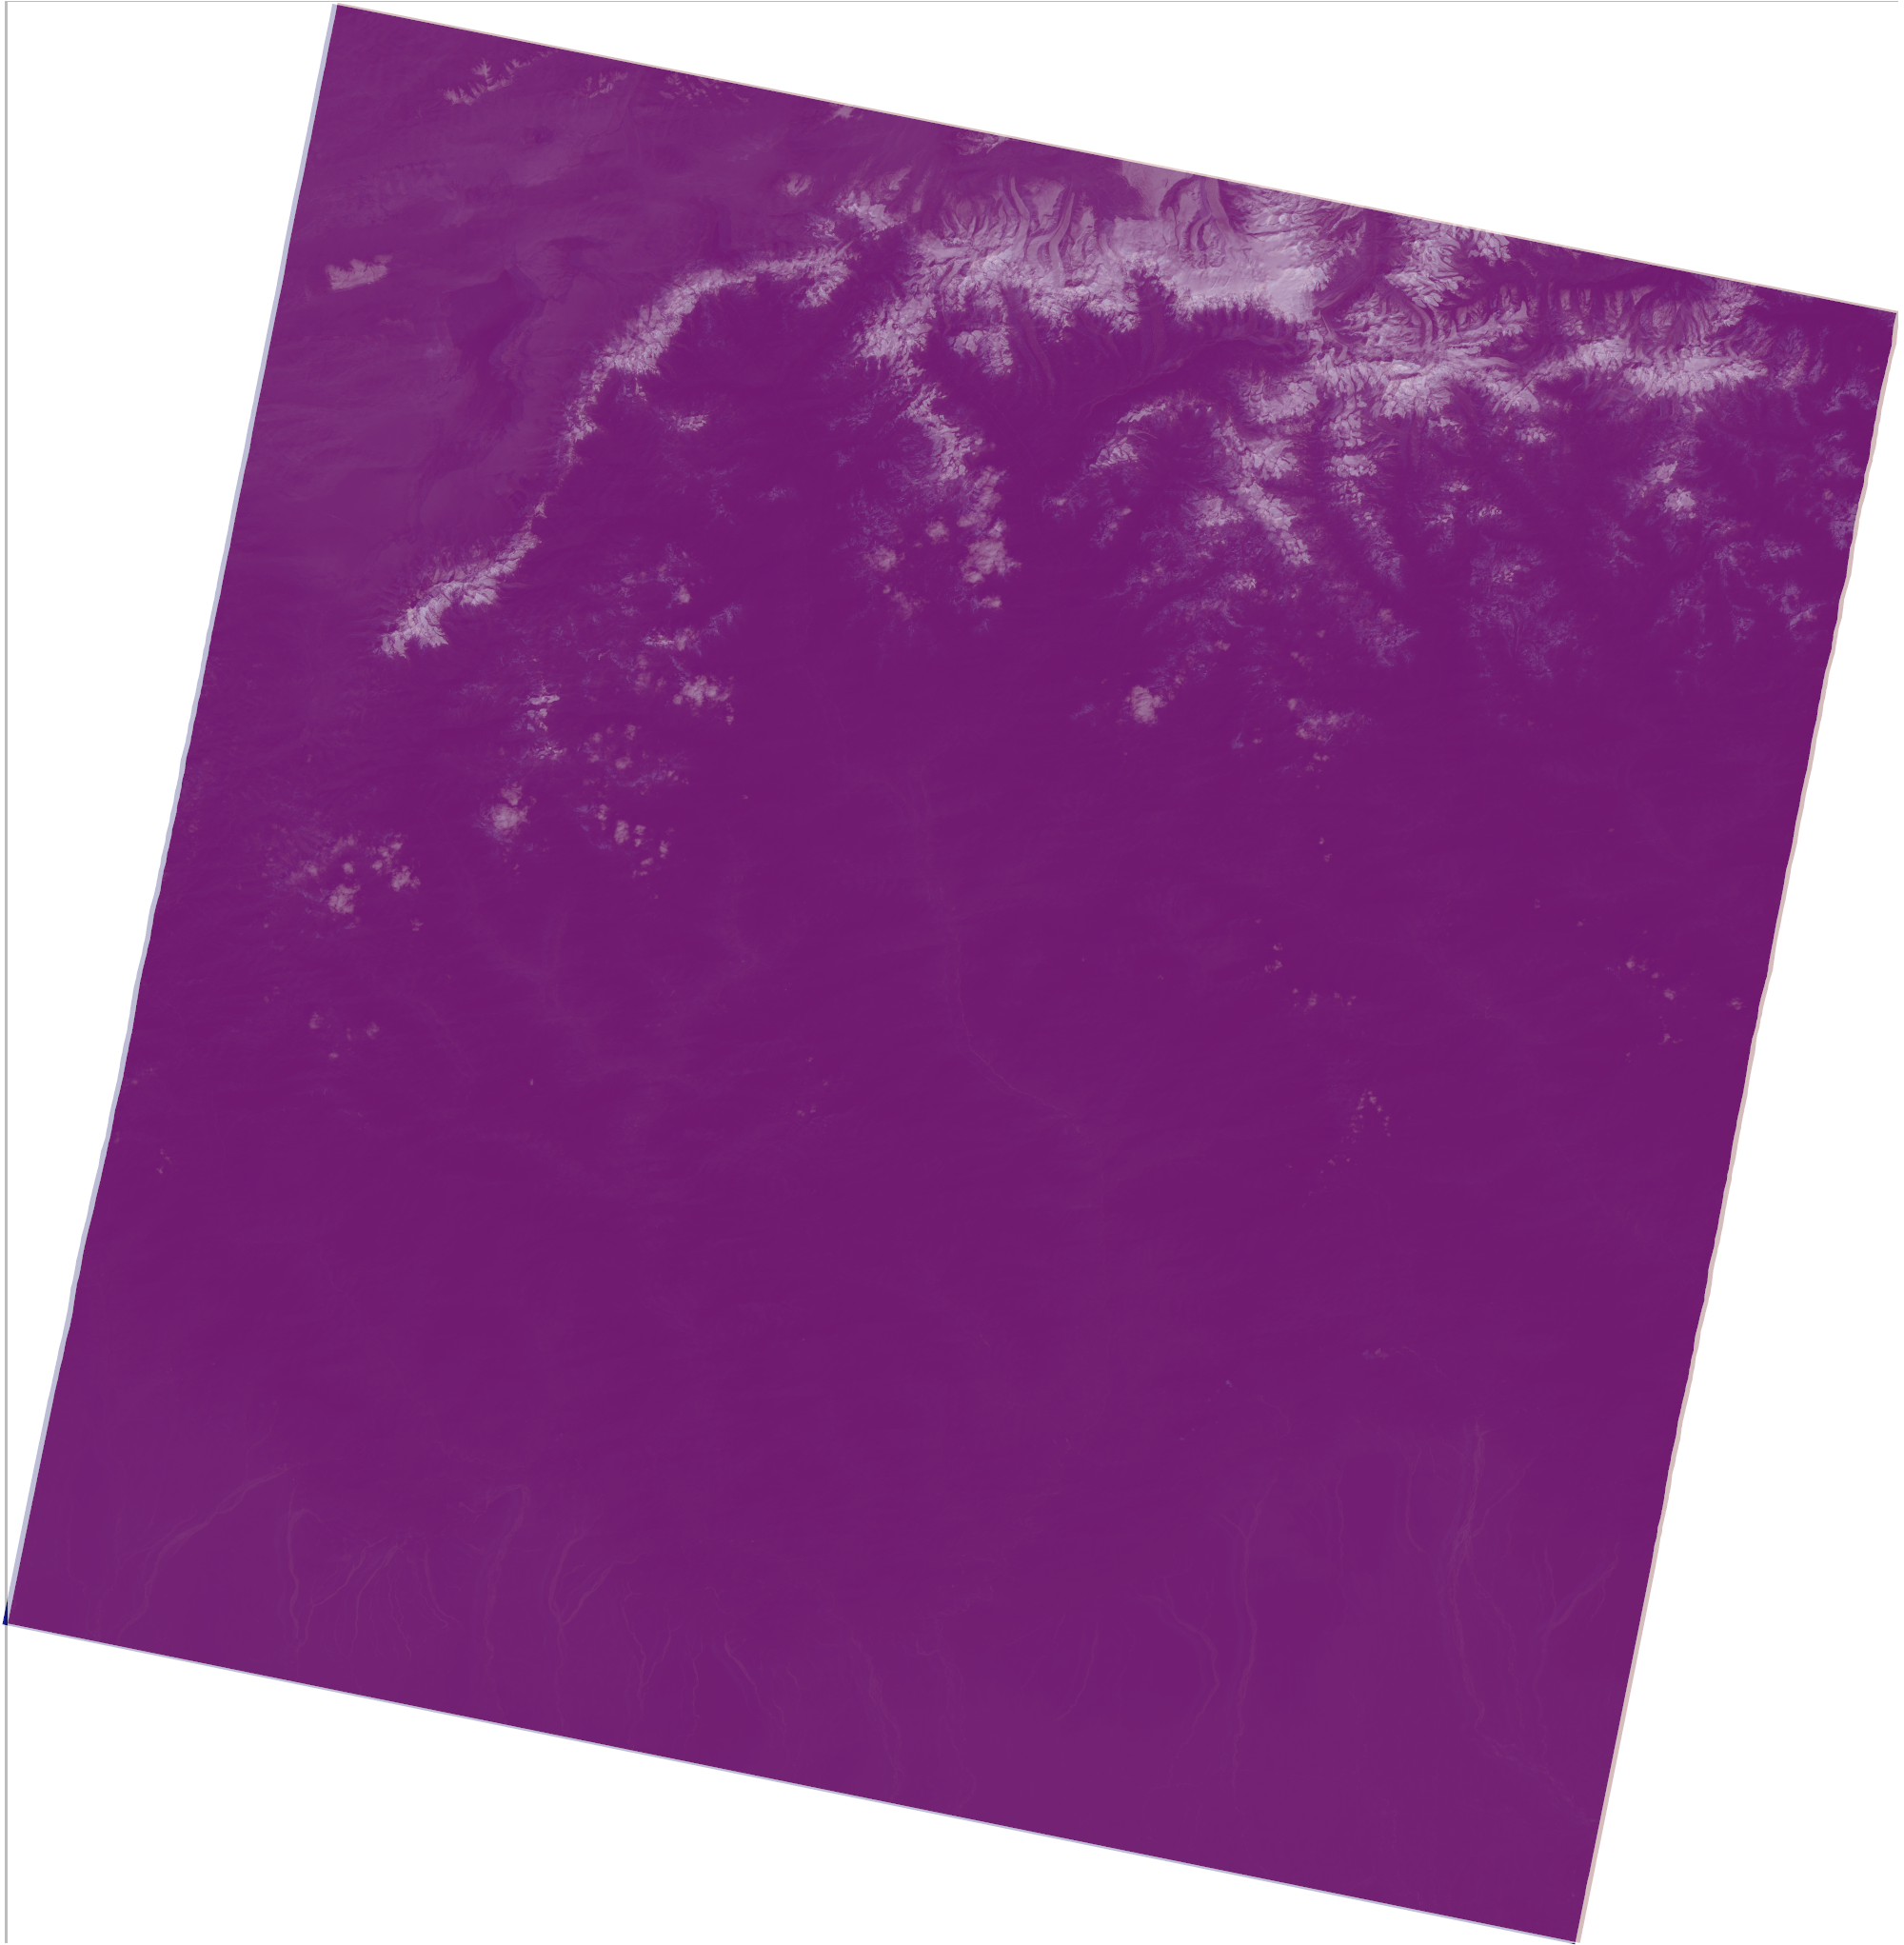
\includegraphics[width=\linewidth]{purple_big_unaligned.png}
  		\endminipage
  		\caption{Two unaligned Landsat 8 scenes, overlapped.}\label{fig:big_unaligned}
  	\end{figure}
  	
  	\begin{figure}[H]
  		\minipage{0.32\textwidth}
  		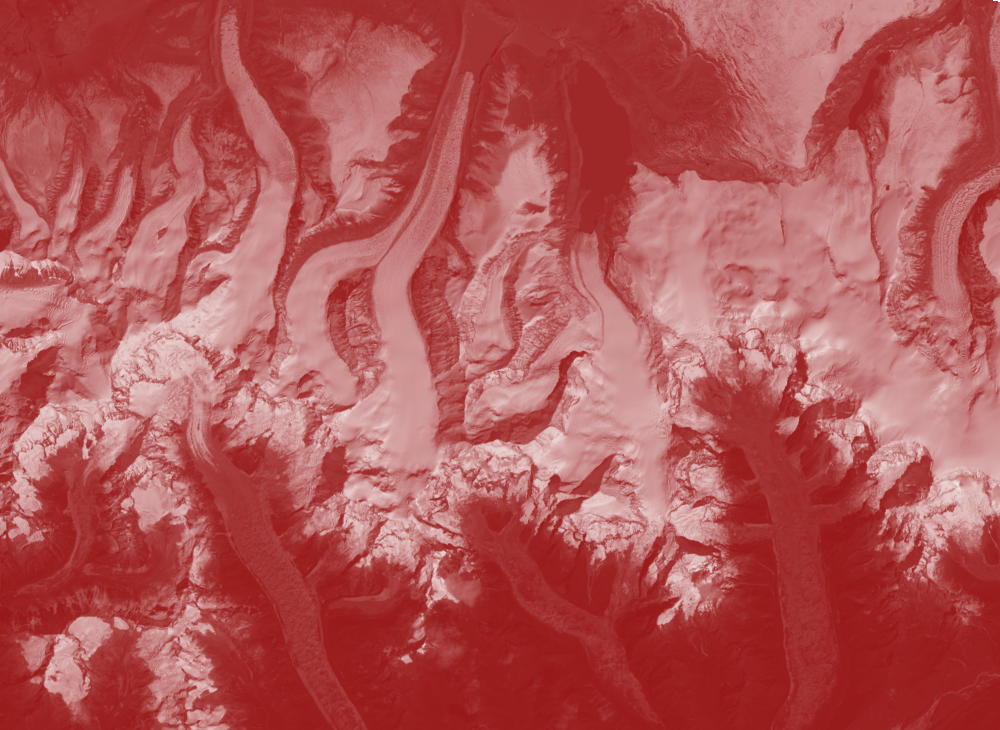
\includegraphics[width=\linewidth]{red_tiny_unaligned.png}
  		\endminipage\hfill
  		\minipage{0.32\textwidth}
  		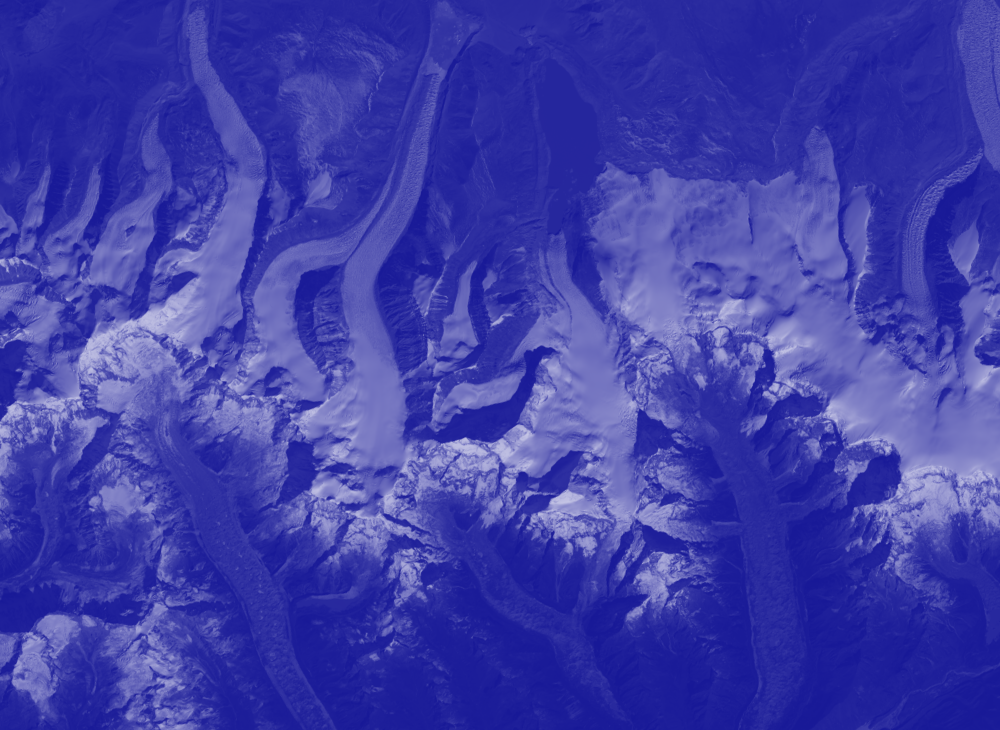
\includegraphics[width=\linewidth]{blue_tiny_unaligned.png}
  		\endminipage\hfill
  		\minipage{0.32\textwidth}%
  		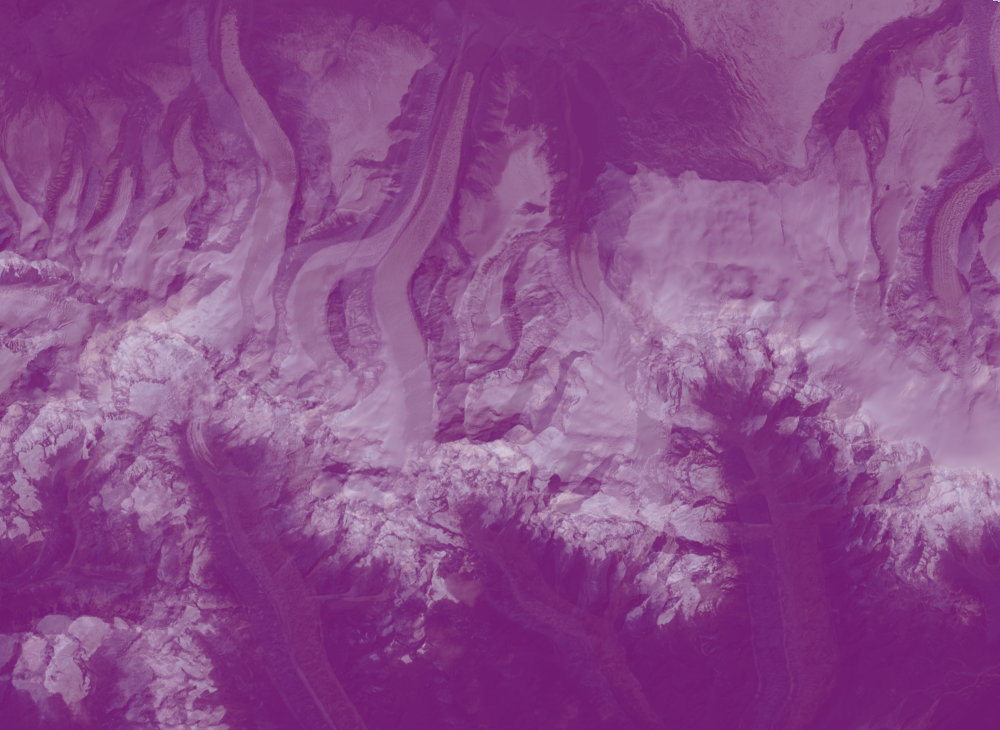
\includegraphics[width=\linewidth]{purple_tiny_unaligned.png}
  		\endminipage
  		\caption{Zoomed in two unaligned Landsat 8 scenes, overlapped.}\label{fig:tiny_unaligned}
  	\end{figure}
  	
  	Given that Landsat 8 has a spatial resolution of 30, each pixel represents 30 meters in the real world. A discrepancy of 100 pixels creates a large spatial error, which lads to errors in determining whether there was snow in the same location between images. A discrepancy even as little creates an unreliable analysis on evolution of snow coverage and glaciers. Therefore, aligning the images is necessary in order to proceed with the results. The following images are the same ones as above, only aligned:
  	
  	
  	\begin{figure}[H]
  		\minipage{0.32\textwidth}
  		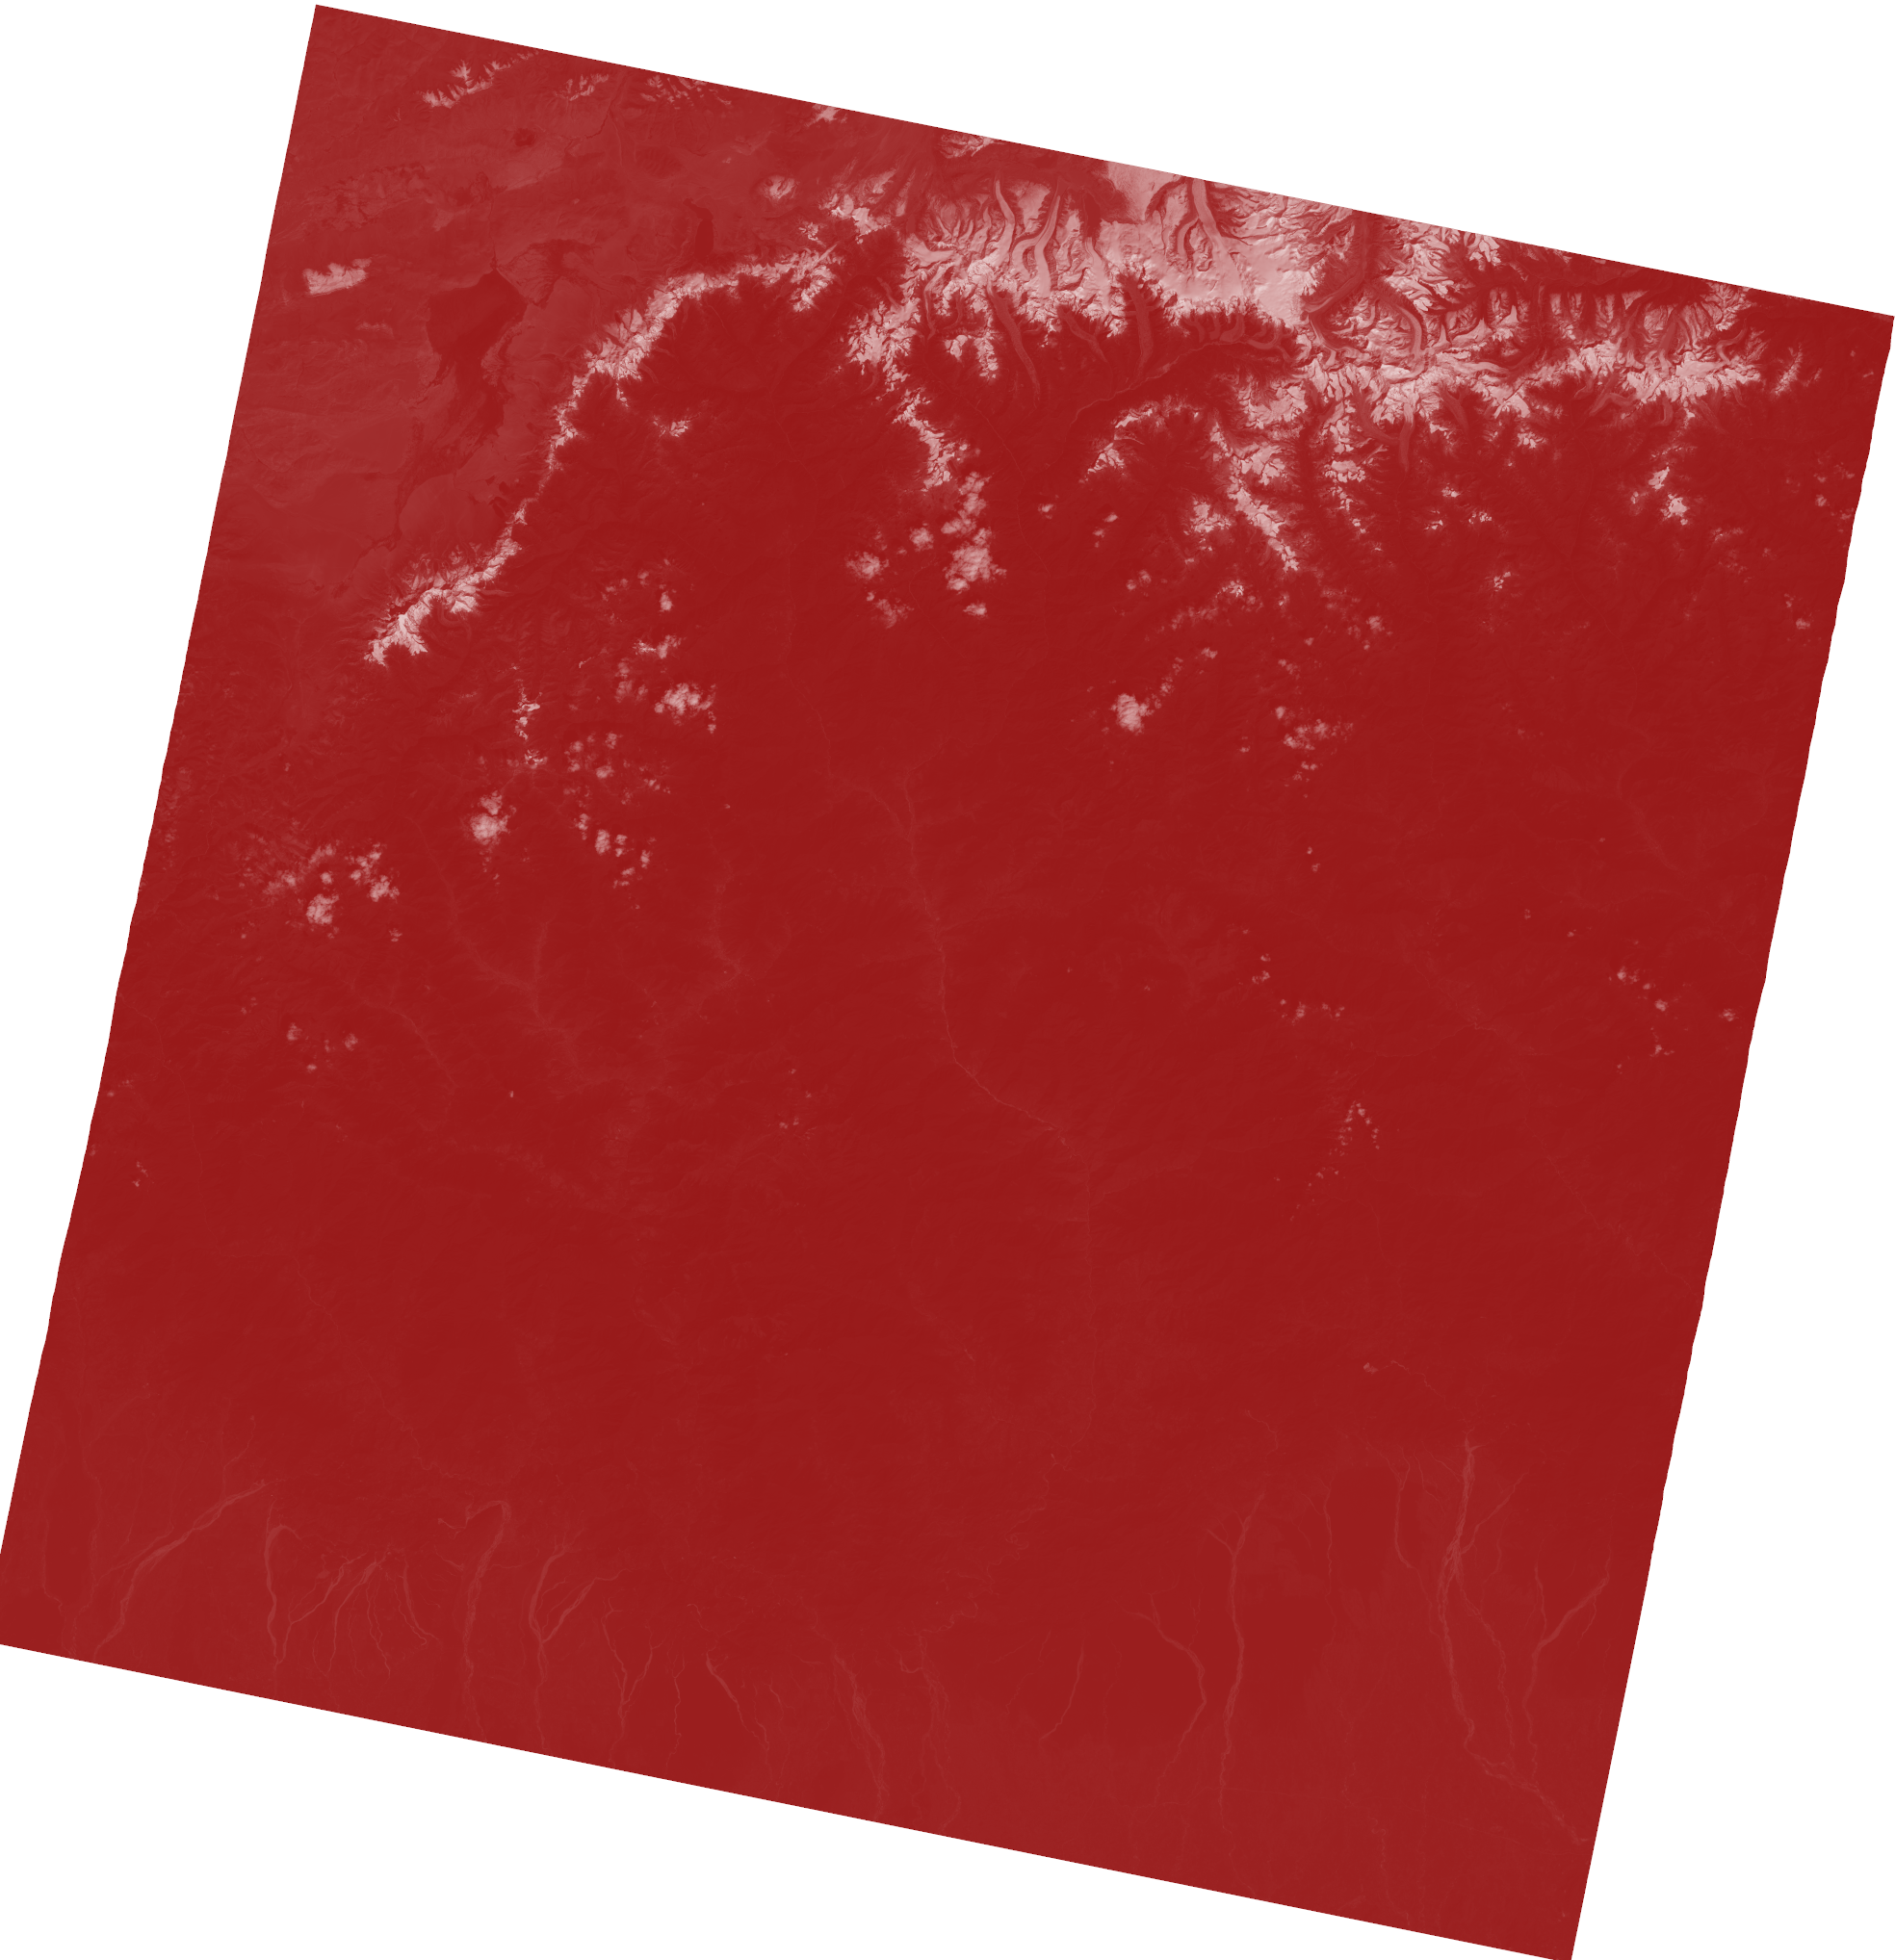
\includegraphics[width=\linewidth]{red_big_aligned.png}
  		\endminipage\hfill
  		\minipage{0.32\textwidth}
  		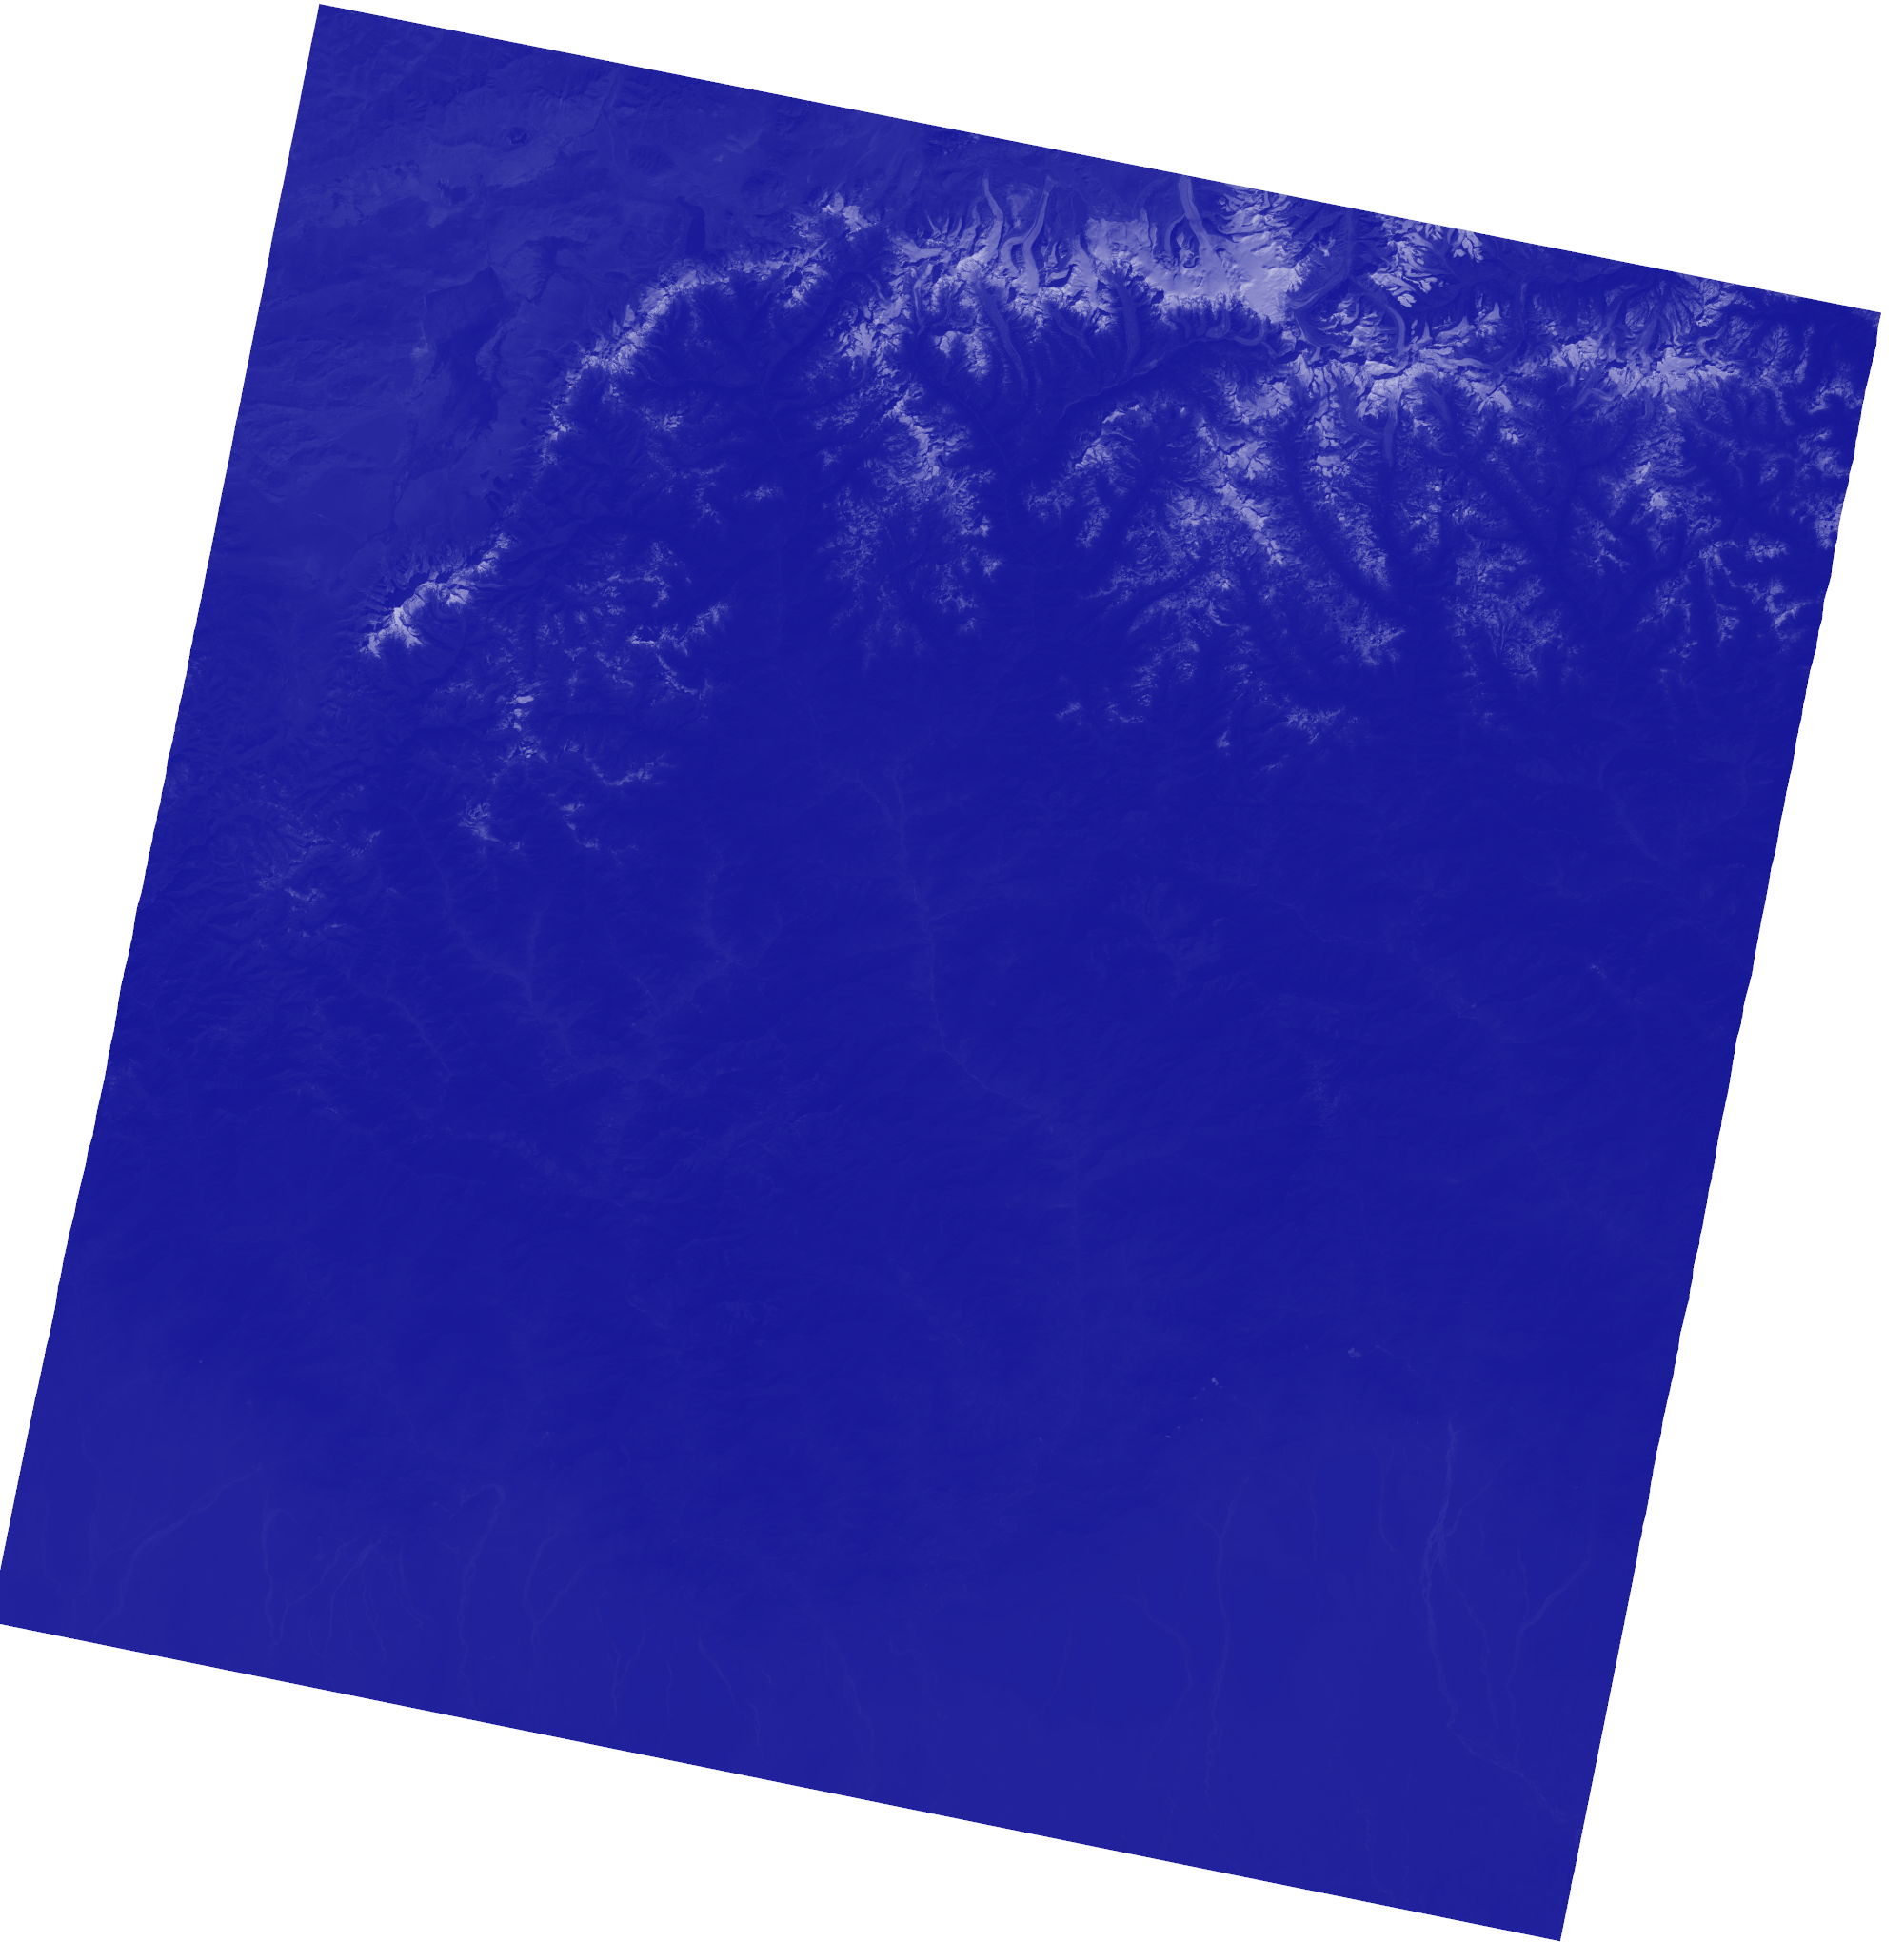
\includegraphics[width=\linewidth]{blue_big_aligned.png}
  		\endminipage\hfill
  		\minipage{0.32\textwidth}%
  		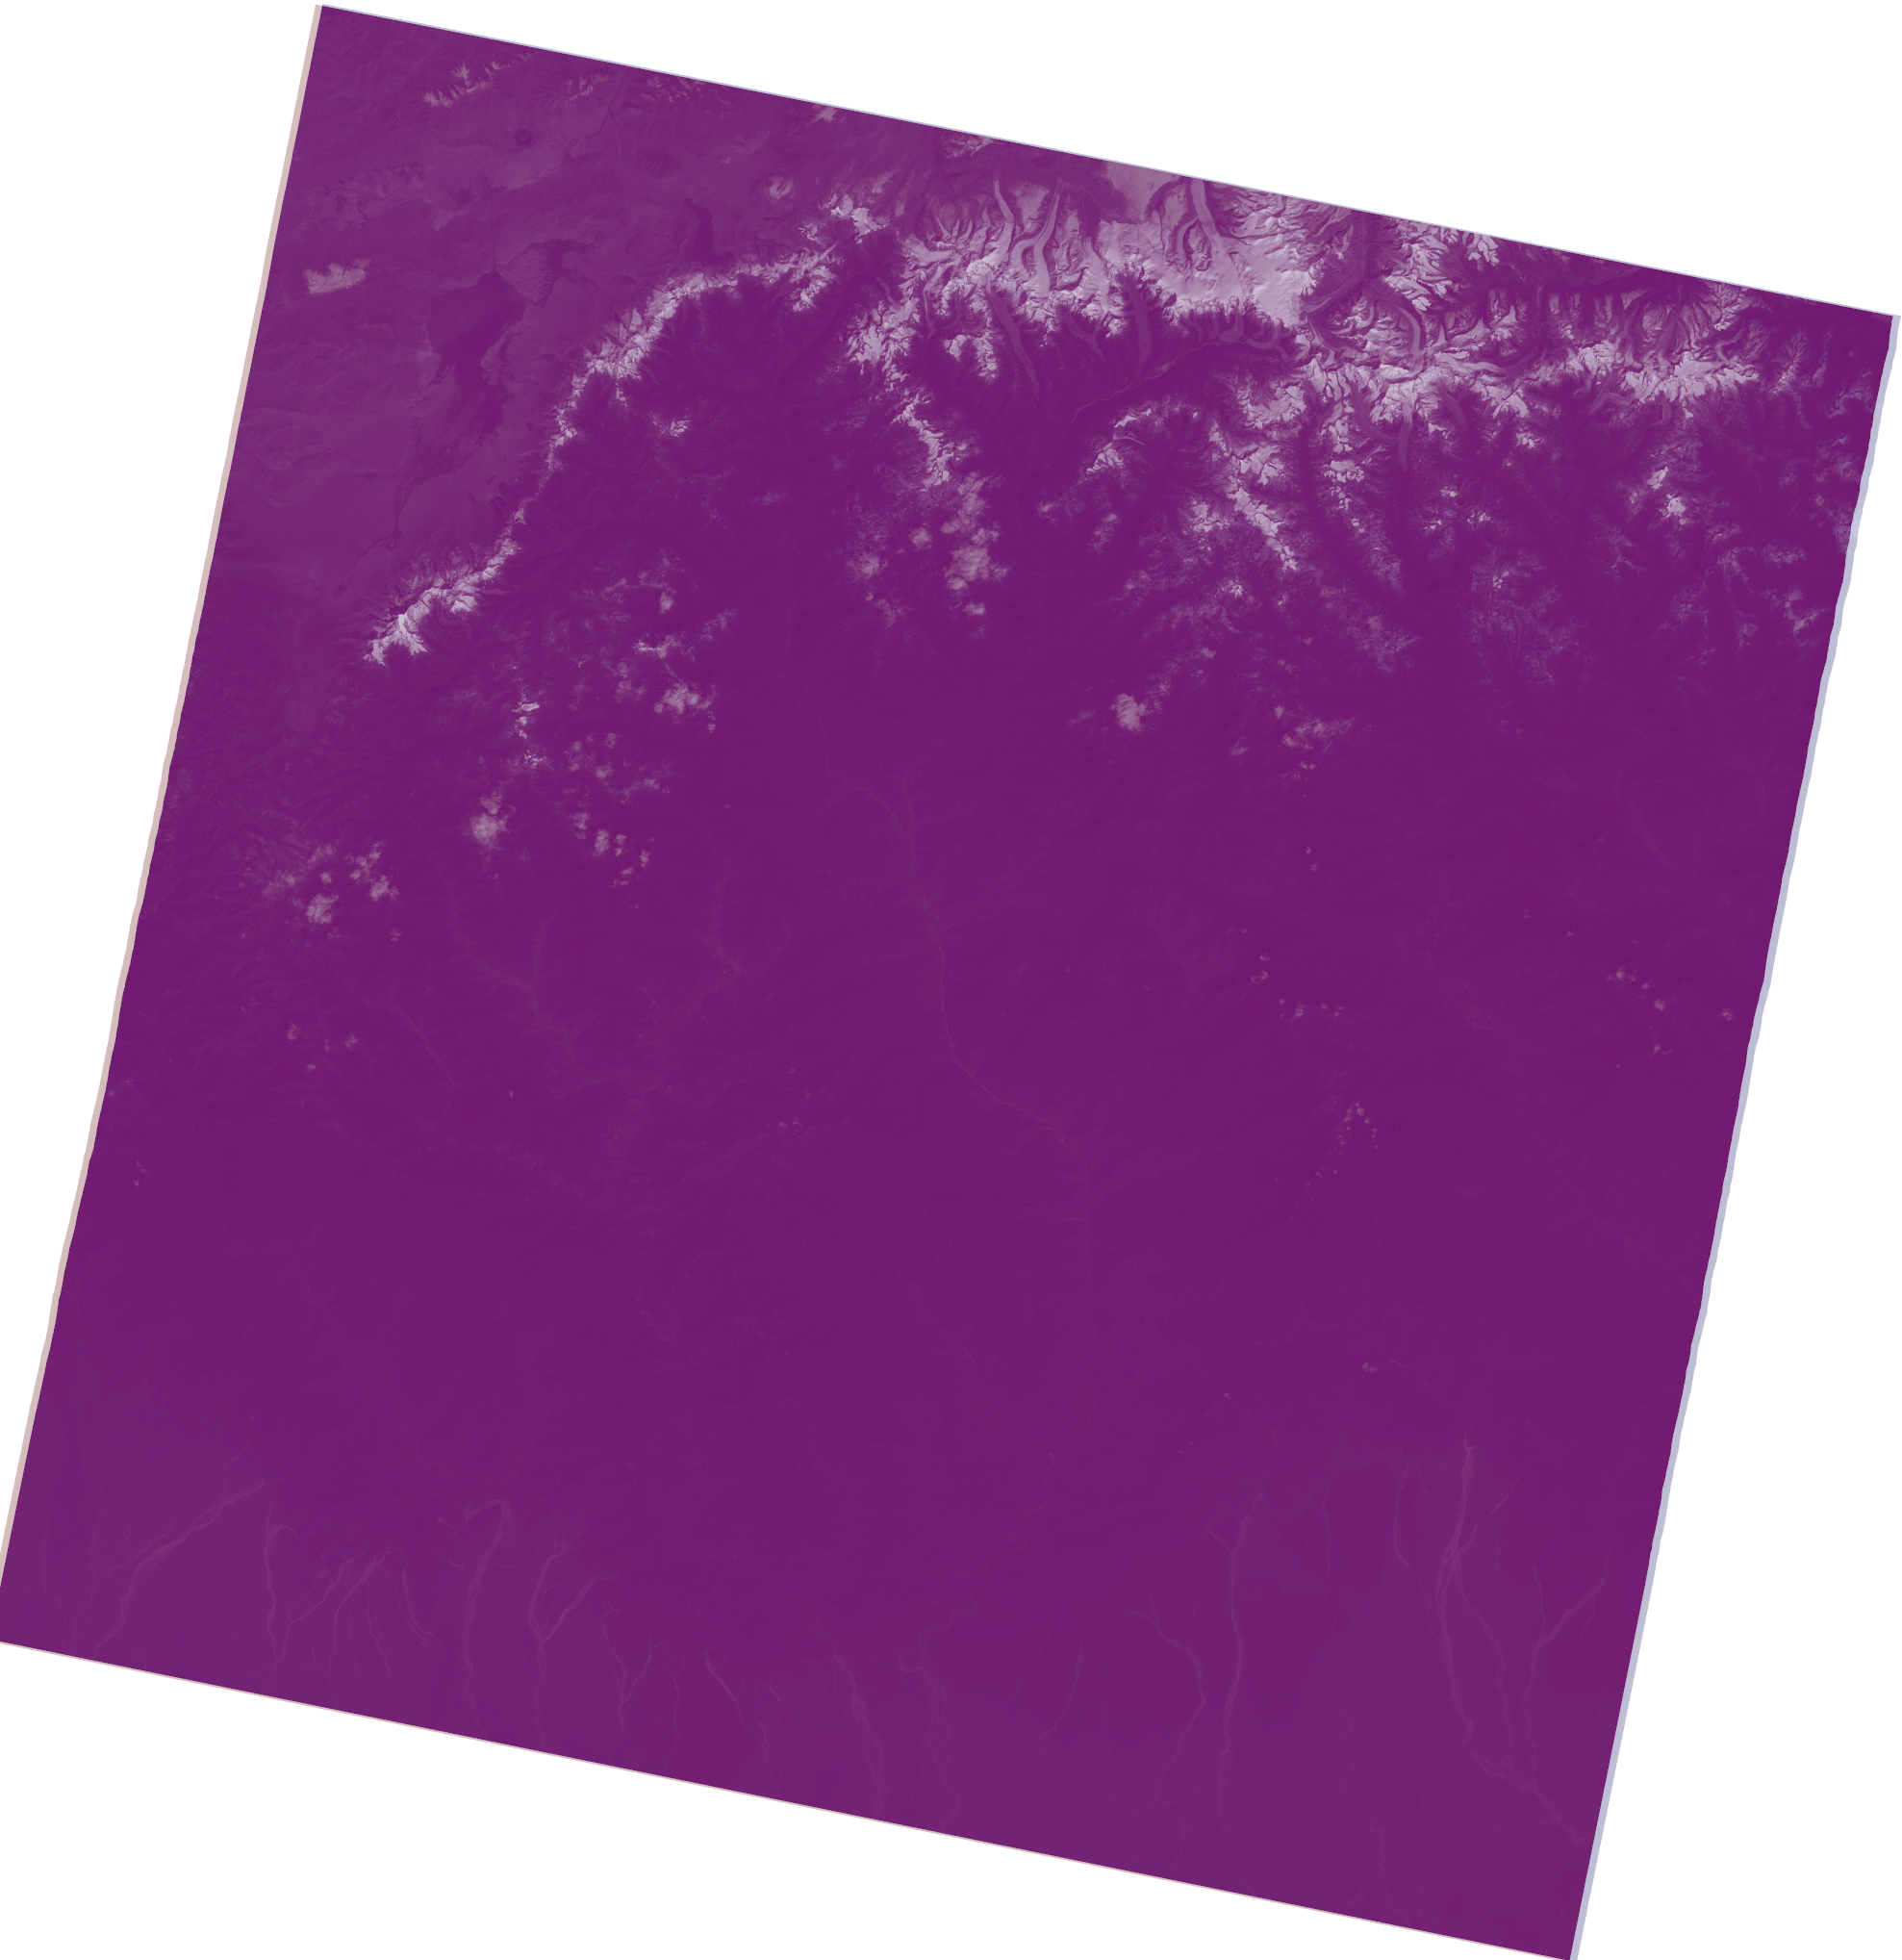
\includegraphics[width=\linewidth]{purple_big_aligned.png}
  		\endminipage
  		\caption{Two aligned Landsat 8 scenes, overlapped.}\label{fig:big_aligned}
  	\end{figure}
  	
  	\begin{figure}[H]
  		\minipage{0.32\textwidth}
  		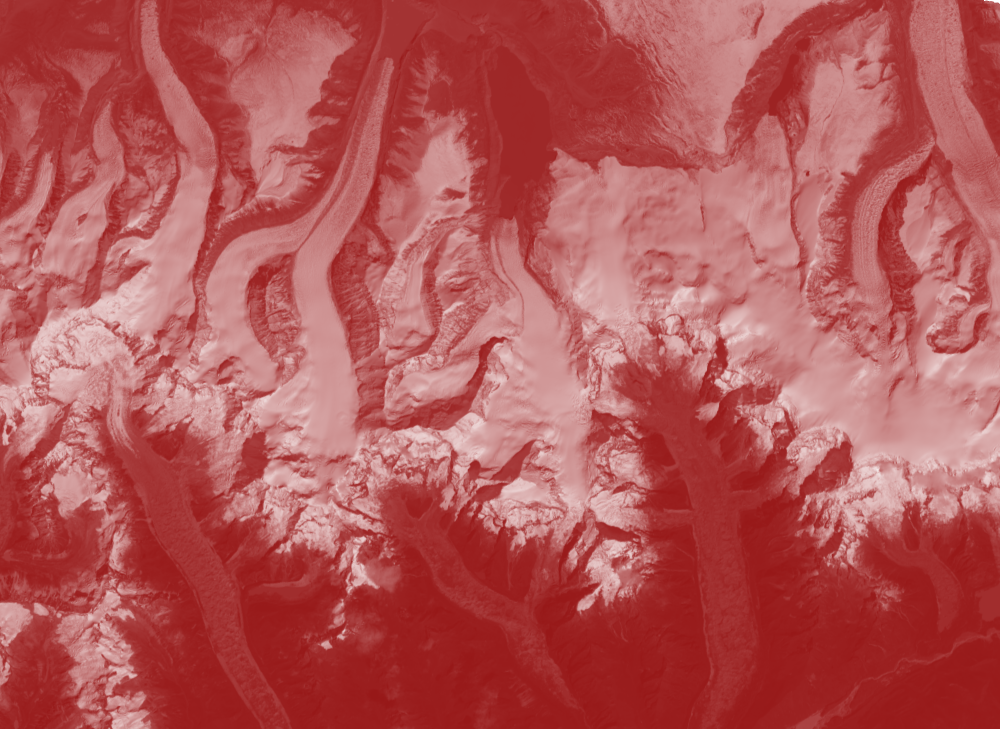
\includegraphics[width=\linewidth]{red_tiny_aligned.png}
  		\endminipage\hfill
  		\minipage{0.32\textwidth}
  		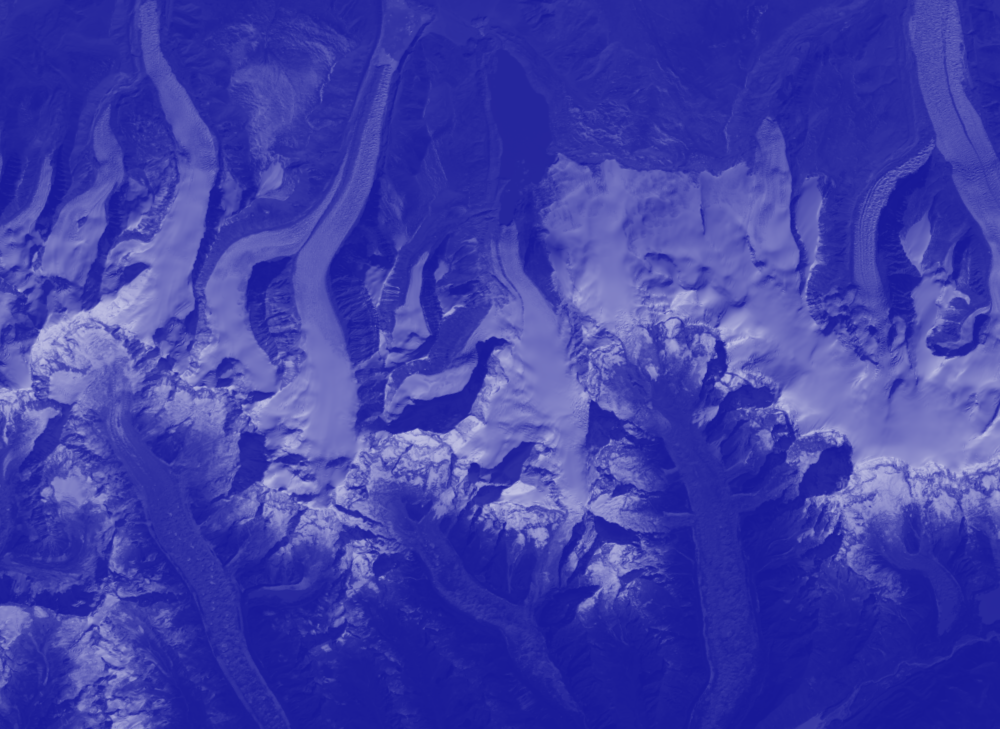
\includegraphics[width=\linewidth]{blue_tiny_aligned.png}
  		\endminipage\hfill
  		\minipage{0.32\textwidth}%
  		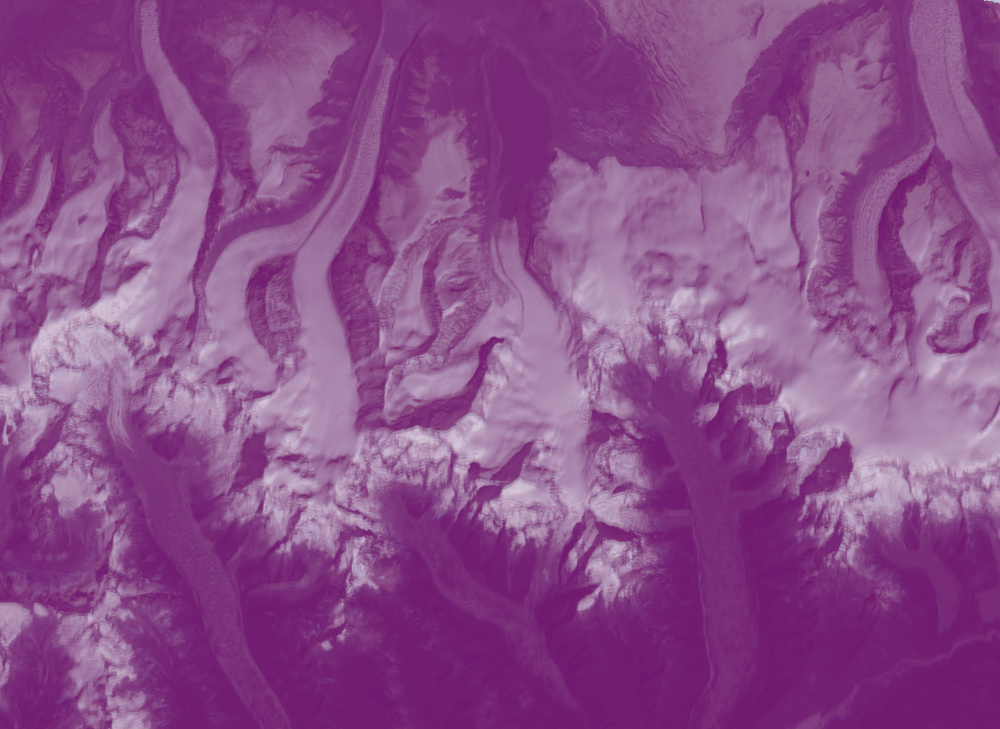
\includegraphics[width=\linewidth]{purple_tiny_aligned.png}
  		\endminipage
  		\caption{Zoomed in two aligned Landsat 8 scenes, overlapped.}\label{fig:tiny_aligned}
  	\end{figure}
  	
  	Several methods for achieving close to perfect alignment results have been used, which will be described in the Design and Implementation section.
  	chapter. The images above have been chosen as example due to the appearance of glacier melting, snow and dry land, which are the characteristics taken in consideration for determining the object appearance or disappearance, as well as its movements in time. By also being very similar, the discrepancy can be easily seen in the initial ones. 
  	The creation of the aligned data set from the initial one ensures that these processing actions can be completed with great results, rather than working on unaligned images. 
  	
  	\subsection{Diference}
  	
  	There are two cases for defining the state of the snow coverage in a satellite image, in our case:
  	\begin{itemize}
  		\item The snow is in movement motion.
  		\item The snow appeared or disappeared suddenly.
  	\end{itemize}
  	Differentiating is between two NDSI images is done in order to detect appearance or disappearance of snow masses or glaciers, which analyzed on a time series of images, highlights the difference of glacier on focus with passing years. Successfully determining the state of objects in scenes leads to information such as how constant the changes are, how fast they are moving, the mass of snow melted and even complete disappearance of some glaciers due to high temperature. The following pictures illustrate glacier and snow masses change, as well as their color maps in order to highlight the changes for visual interpretation:
  	\begin{figure}[H]
  		\minipage{0.48\textwidth}
  		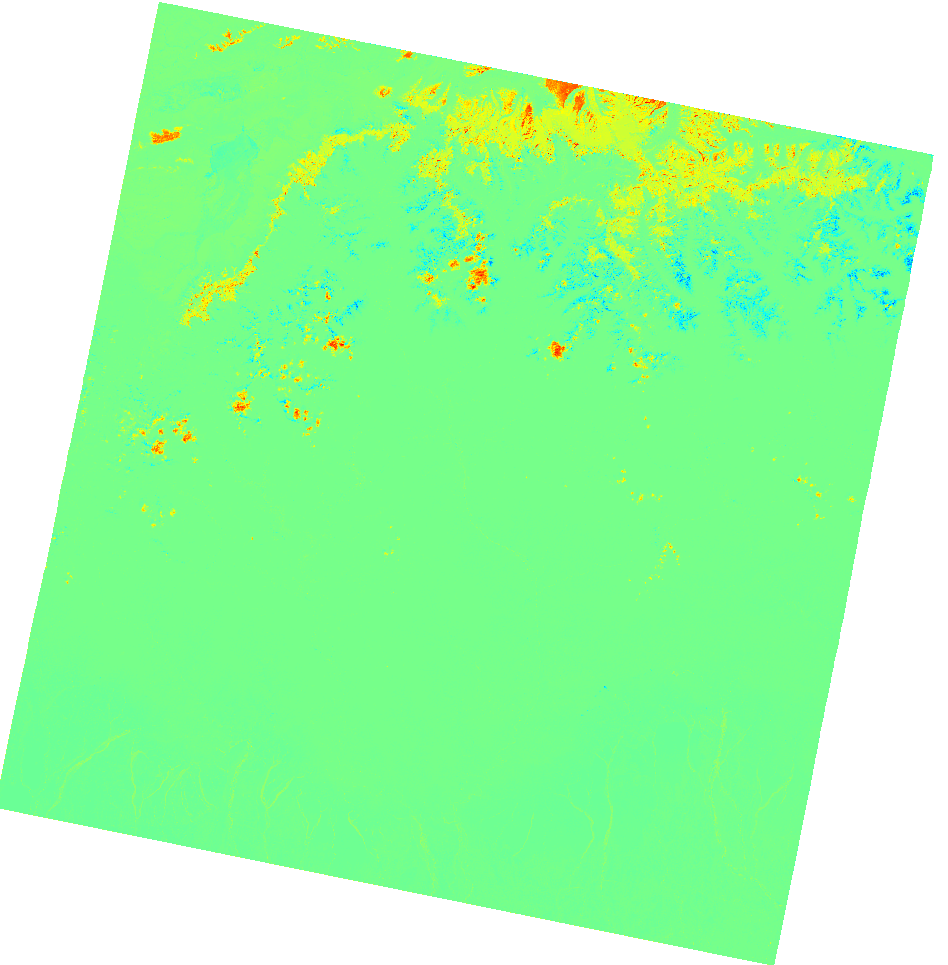
\includegraphics[width=\linewidth]{difference.png}
  		\endminipage\hfill
  		\minipage{0.48\textwidth}
  		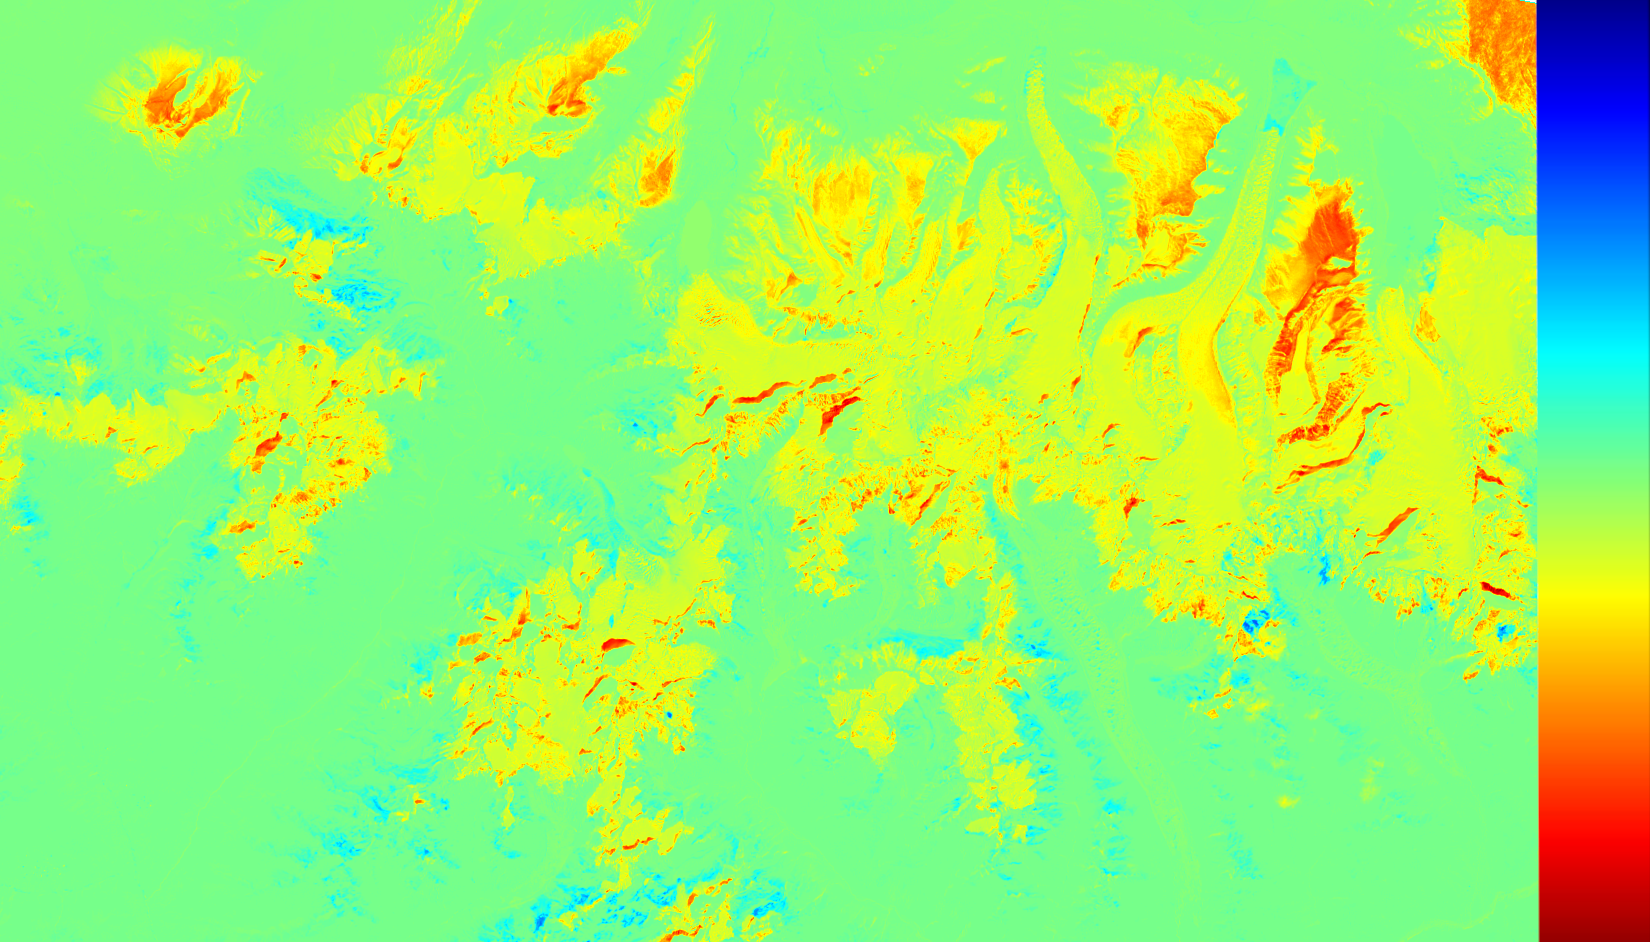
\includegraphics[width=\linewidth]{diff_tiny.png}
  		\endminipage\hfill
  		\caption{Difference for object state.}\label{fig:diff_img}
  	\end{figure}
  	
  	\subsection{Movement}
  	The movement of objects from an image is equally important in extracting information, such as the angle of the rotation, its magnitude, information about the speed of the changes and their scale. Applied on an NDSI scene, the following result is obtained:
  	\begin{figure}[H]
  		\minipage{0.48\textwidth}
  		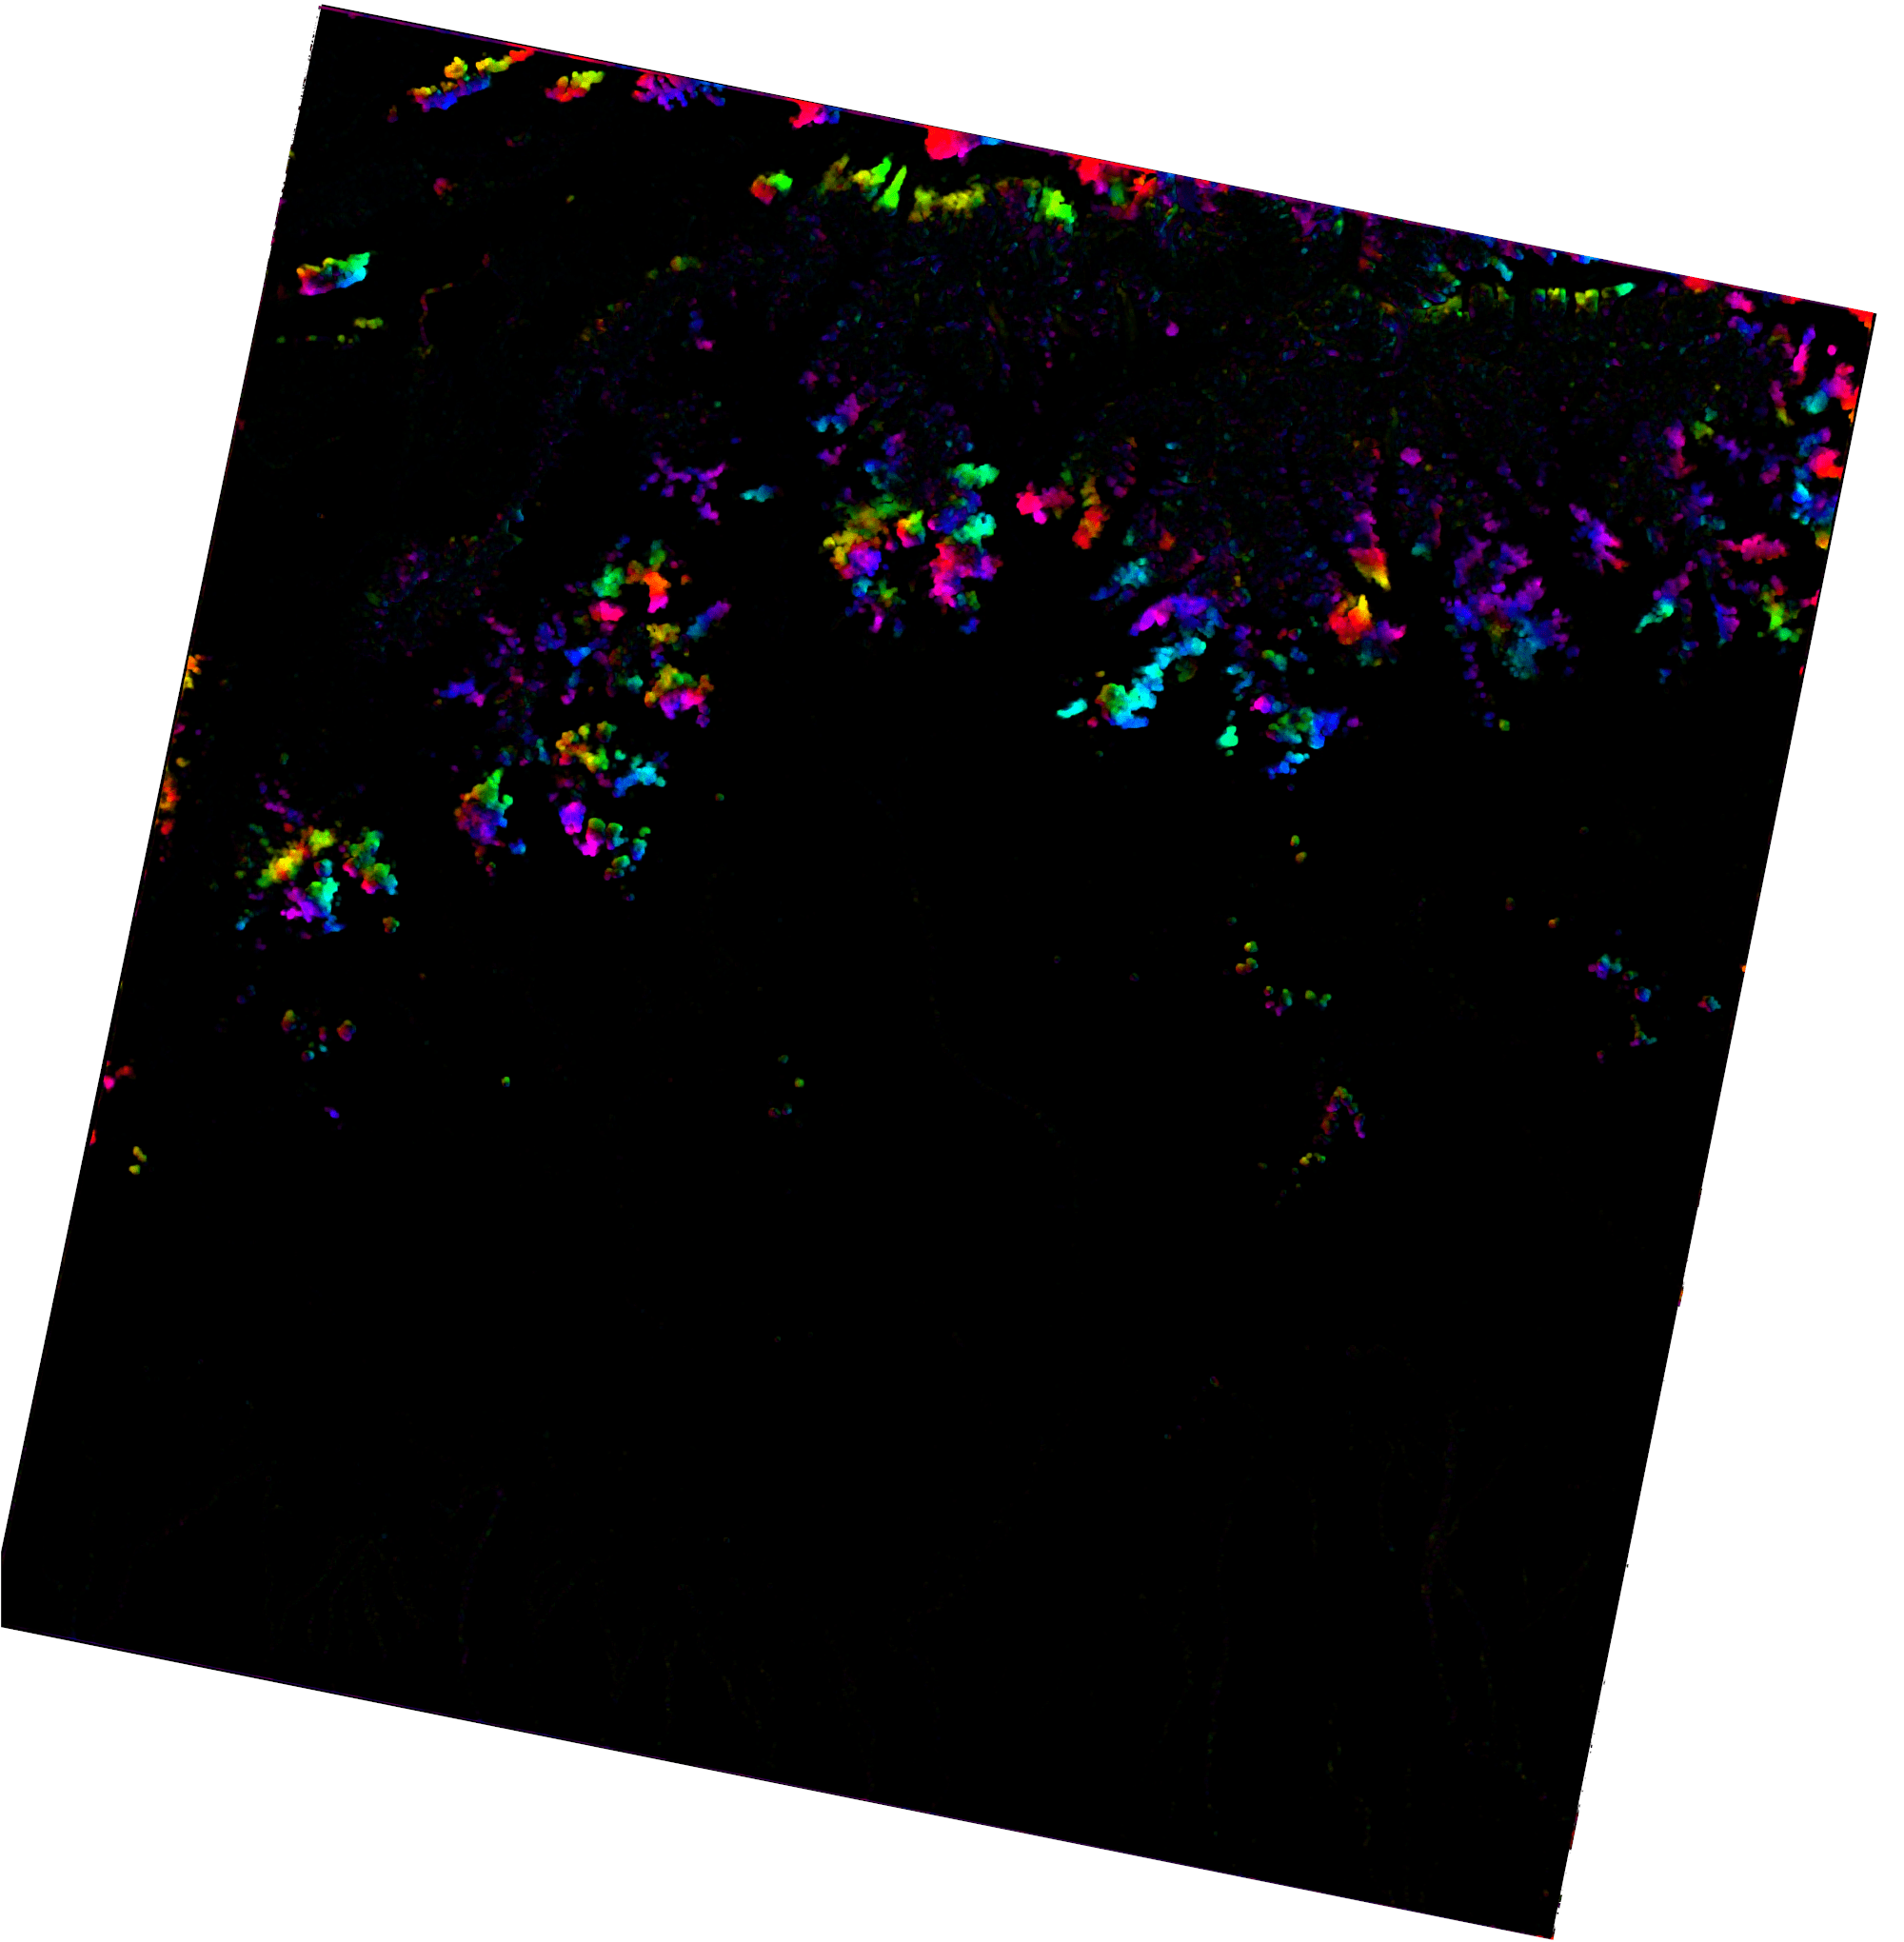
\includegraphics[width=\linewidth]{move_big.png}
  		\endminipage\hfill
  		\minipage{0.48\textwidth}
  		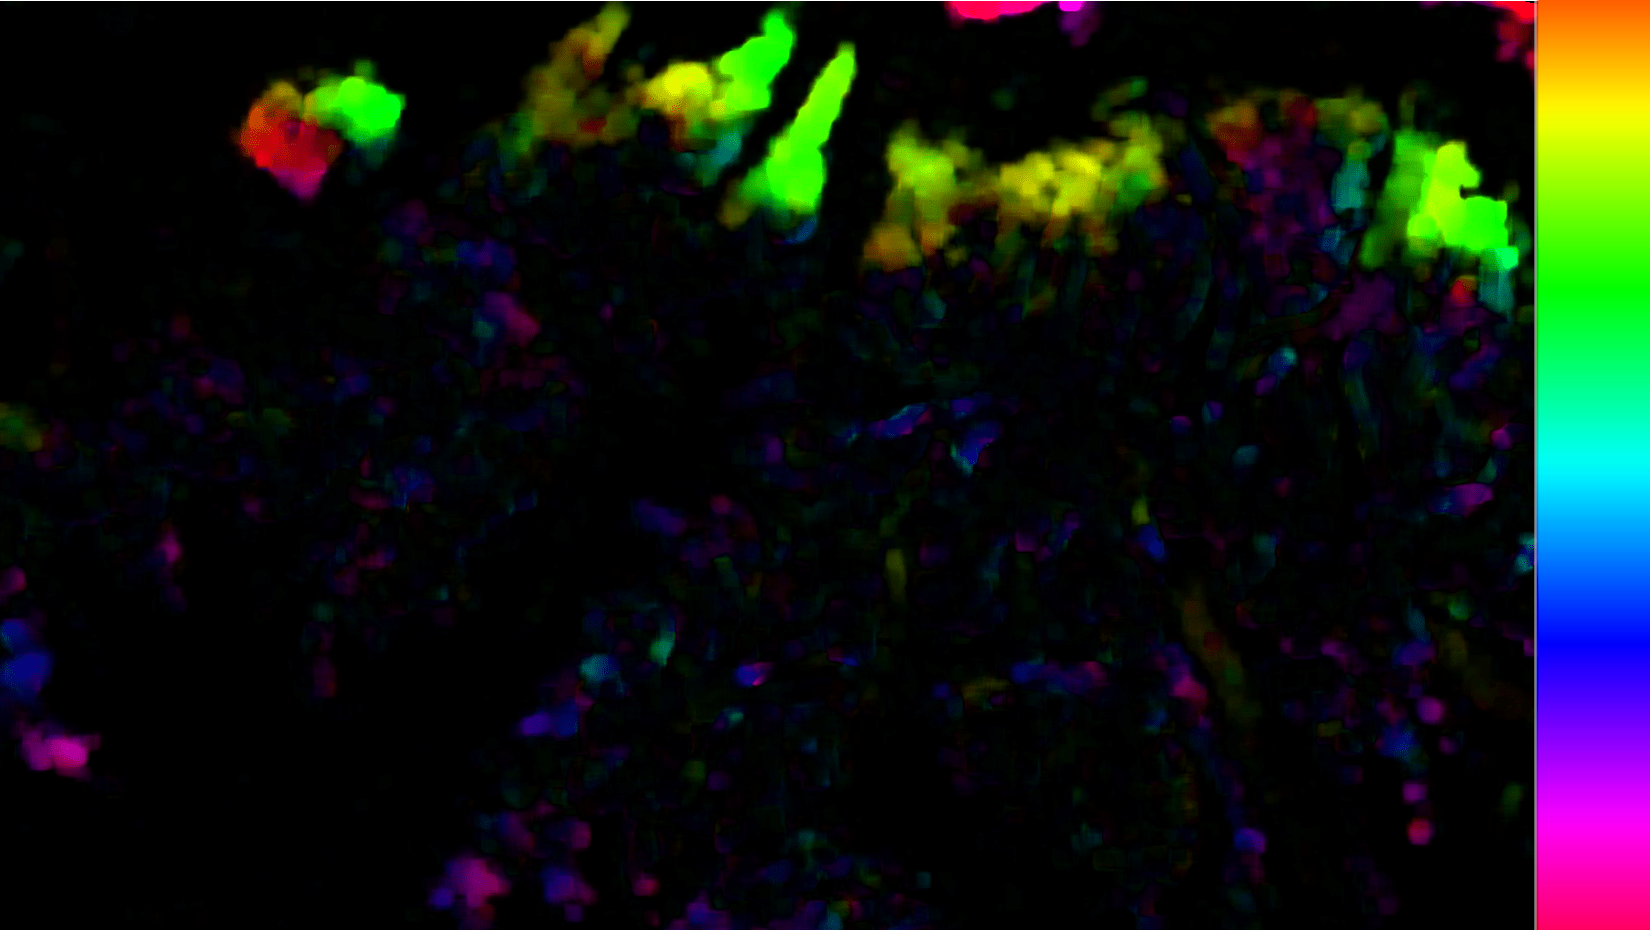
\includegraphics[width=\linewidth]{move_tiny.png}
  		\endminipage\hfill
  		\caption{Difference for object movement.}\label{fig:move_img}
  	\end{figure}
	
	
	
	
	
	\section{The user interface and guide}
	
	The user has two options regarding the interface, for better convenience, since some users are more inclined to using a graphical user interface rather than a command line one. The following are the options:
	\begin{itemize}
		\item \textbf{Command Line Interface (CLI)}
		\item \textbf{Graphical User Interface (GUI)}
	\end{itemize}
	
	The \textbf{command line interface} has been chosen for reasons such as \textbf{simplicity, efficiency, faster results}, which can be opted for by users which have a higher experience in programming and dealing with such an interface.Command line applications have been used since the development of the first computers and are still being used today for the same reasons specified before, as well as access to other programs and features in the system which would be hardly accessible to graphical user interfaces. Since the thesis application is more process driven rather than having many visual use cases, opting for keeping a simple command line interface was the best choice in the case of those who which to achieve simpler and faster results.
	
	The \textbf{graphical user interface} is taken as an options for users which do not have much interaction with the command line environment, rather being used to GUI's. By including this option, the number of possible users is enlarged, including also the ones which are not that experienced in the IT field, but still want to use the application without much trouble.
	
	We will describe each process separately, with their GUI and CLI interfaces.
	\definecolor{babyblue}{rgb}{0.54, 0.81, 0.94}
	
	\subsection{Download GUI}
	The download process can be started by pressing \textbf{START PROCESS} button, and stopped with \textbf{STOP PROCESS} one. The diagram which represents the interaction with the graphical user interface, as well as the command line one can be found in 3.14 figure. The displaying from command line can be started as:
	
	\begin{center}
		\begin{lstlisting}[language=bash,
		backgroundcolor = \color{babyblue}]
		python3 main.py download --csv util/files/wgi_feb2012.csv --dir /path/to/download/ -j 3
		\end{lstlisting}
	\end{center}
	
	\subsection{Process GUI}
	The processing can be started by pressing \textbf{START PROCESS} button, and stopped with \textbf{STOP PROCESS} one. The diagram which represents the interaction with the graphical user interface, as well as the command line one can be found in 3.15 figure. The displaying from the command line can be started as:
	
	\begin{center}
		\begin{lstlisting}[language=bash,
		backgroundcolor = \color{babyblue}]
		python3 main.py download python3 main.py process --input /path/to/input/images --output /path/to/download/ -j 3
		\end{lstlisting}
	\end{center}
	
	\subsection{Display GUI}
	The displaying of the results can be started by pressing \textbf{DISPLAY} button, and stopped with the \textbf{EXIT} button from the graphic pop-up or its own. The display interface prints the \textbf{statistical information} processed from calculating the NDSI, and generates a \textbf{prediction of snow coverage}, displaying the results in an interactive plot. By pressing on a plot entry, the \textbf{difference and movement images} are created. The diagram which represents the interaction with the graphical user interface, as well as the command line one can be found in 3.16 figure. The displaying from the command line can be started as:
	
	\begin{center}
		\begin{lstlisting}[language=bash,
		backgroundcolor = \color{babyblue}]
		python3 main.py display --csv /path/to/csv/ndsi_144_039.csv  /path/to/download/images -j 3
		\end{lstlisting}
	\end{center}
	
	
	\section{Difference and Movement GUI}
	The calculation of difference and movement images can be triggered by clicking two of the items found in the interactive plot. The following diagram represents the interaction with the graphical user interface.
	
	\begin{figure}[H]
		\centering
		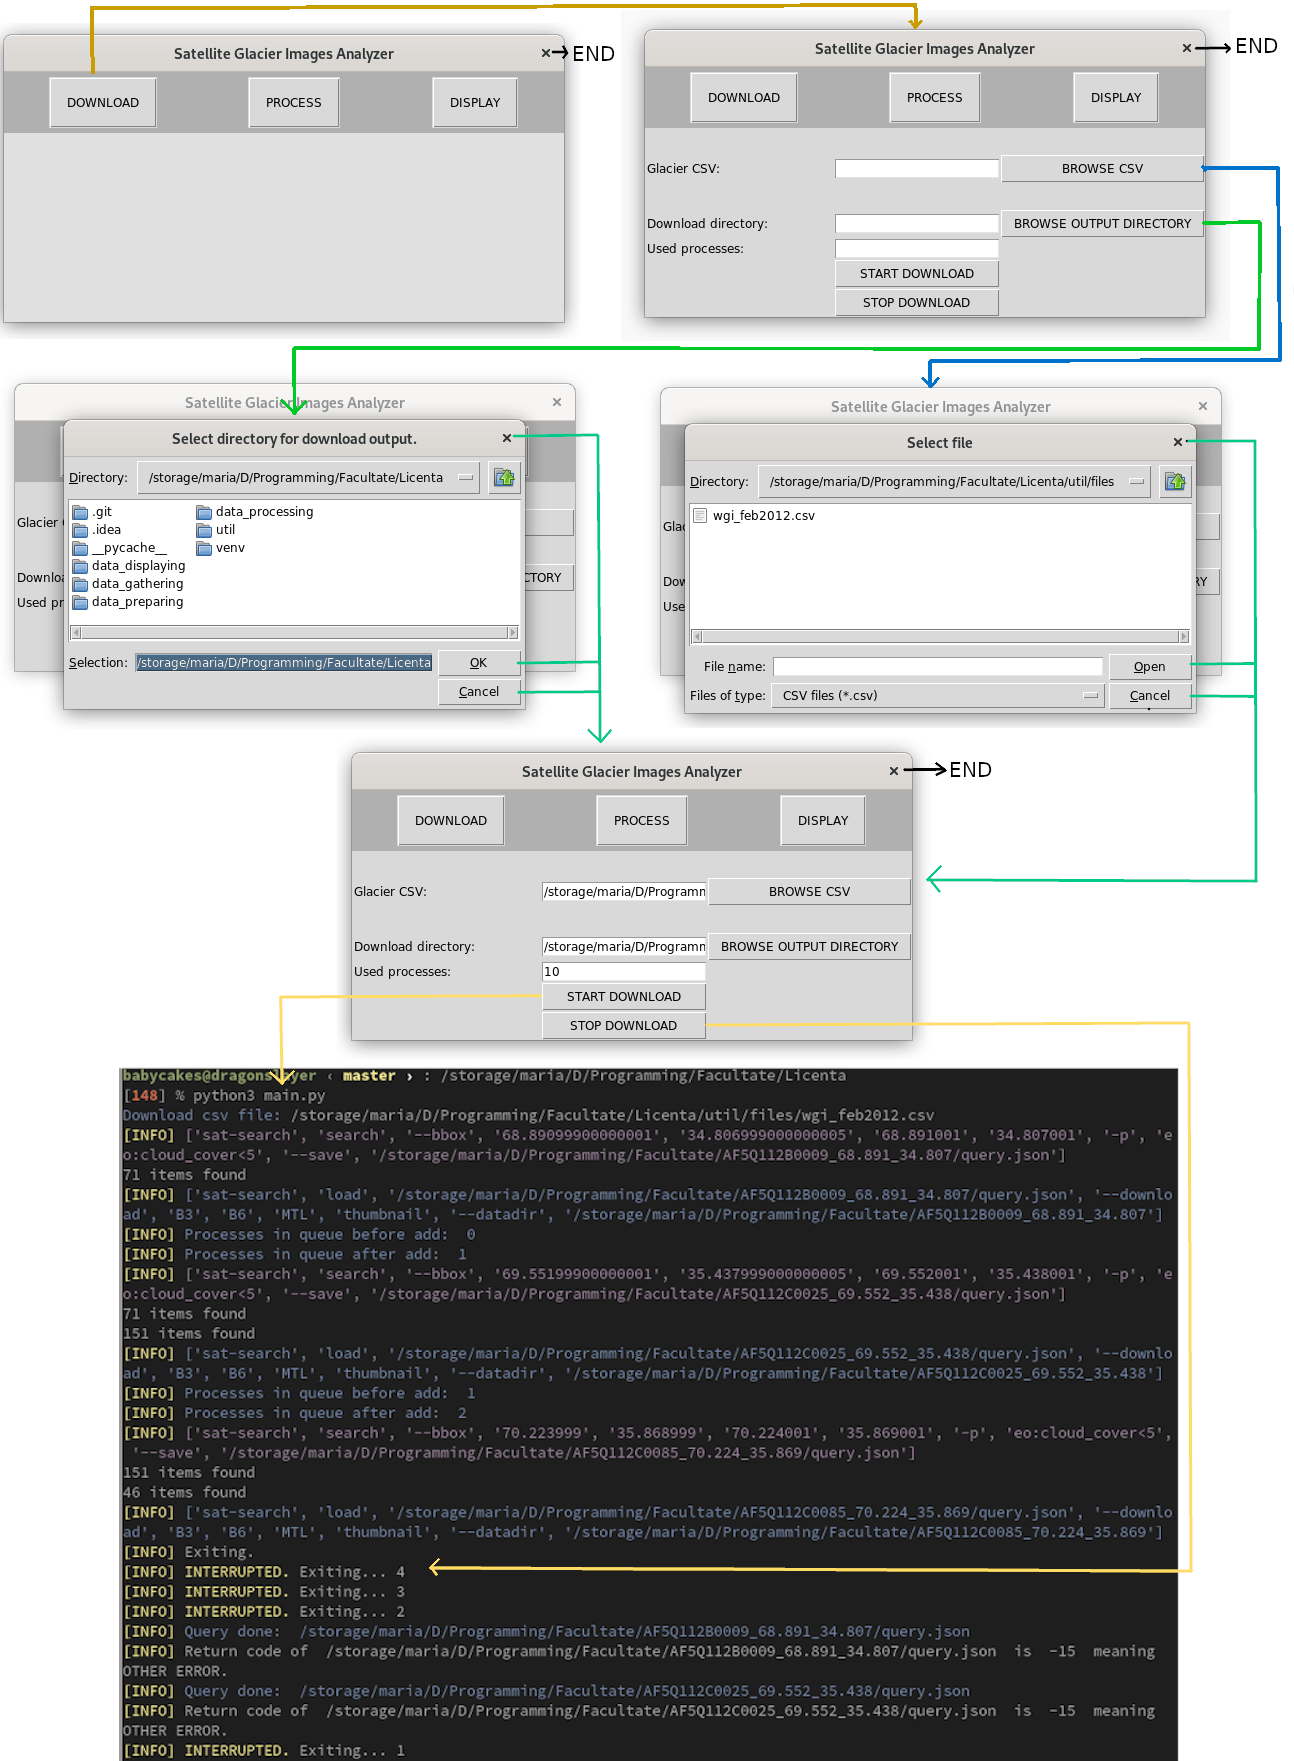
\includegraphics[scale=1.5]{download_gui_cmd.png}
		\caption{Download CLI and GUI diagram.}
		\label{fig:download_gui}
	\end{figure}
	
	\begin{figure}[H]
		\centering
		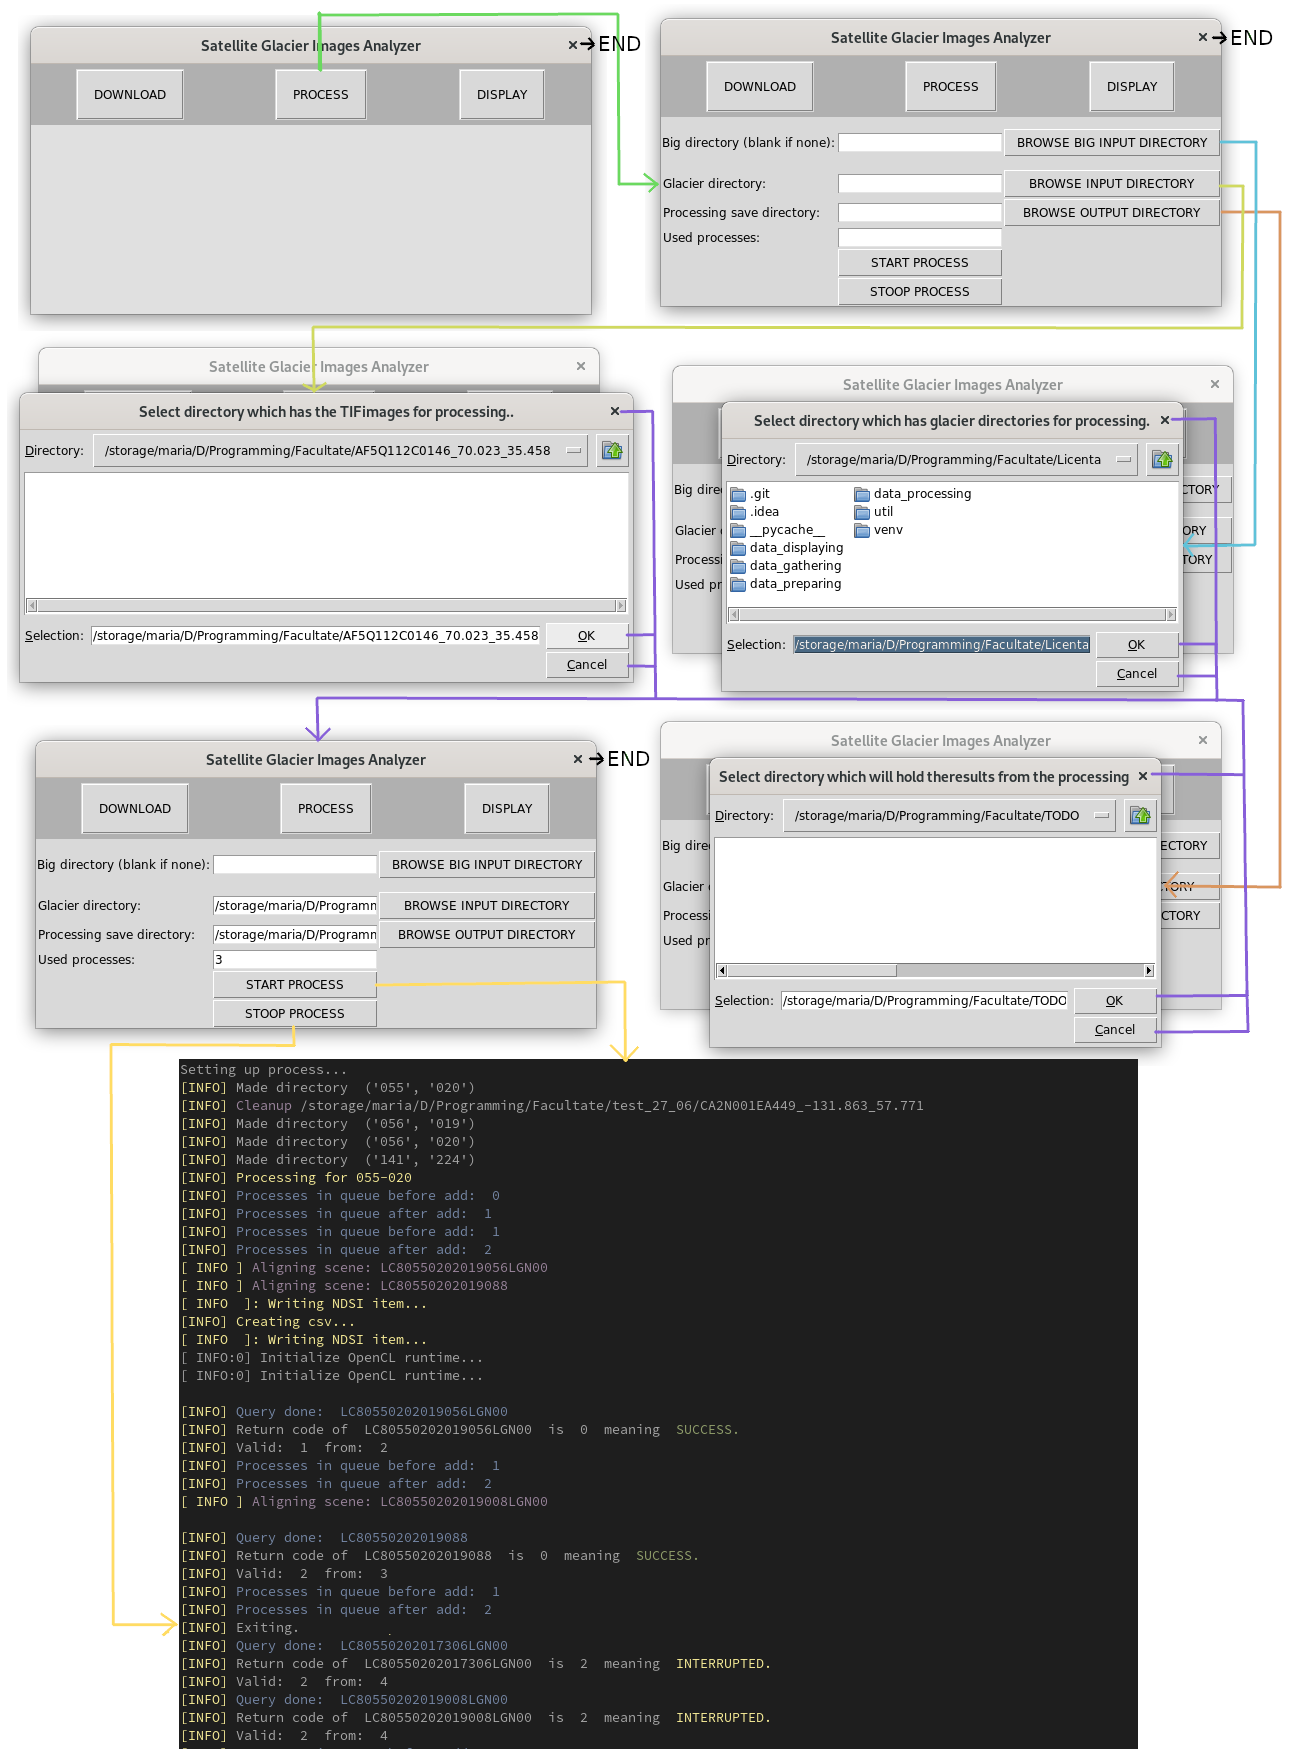
\includegraphics[scale=1.5]{process_cmd_gui.png}
		\caption{Process CLI and GUI diagram.}
		\label{fig:process_gui}
	\end{figure}
	
	\begin{figure}[H]
		\centering
		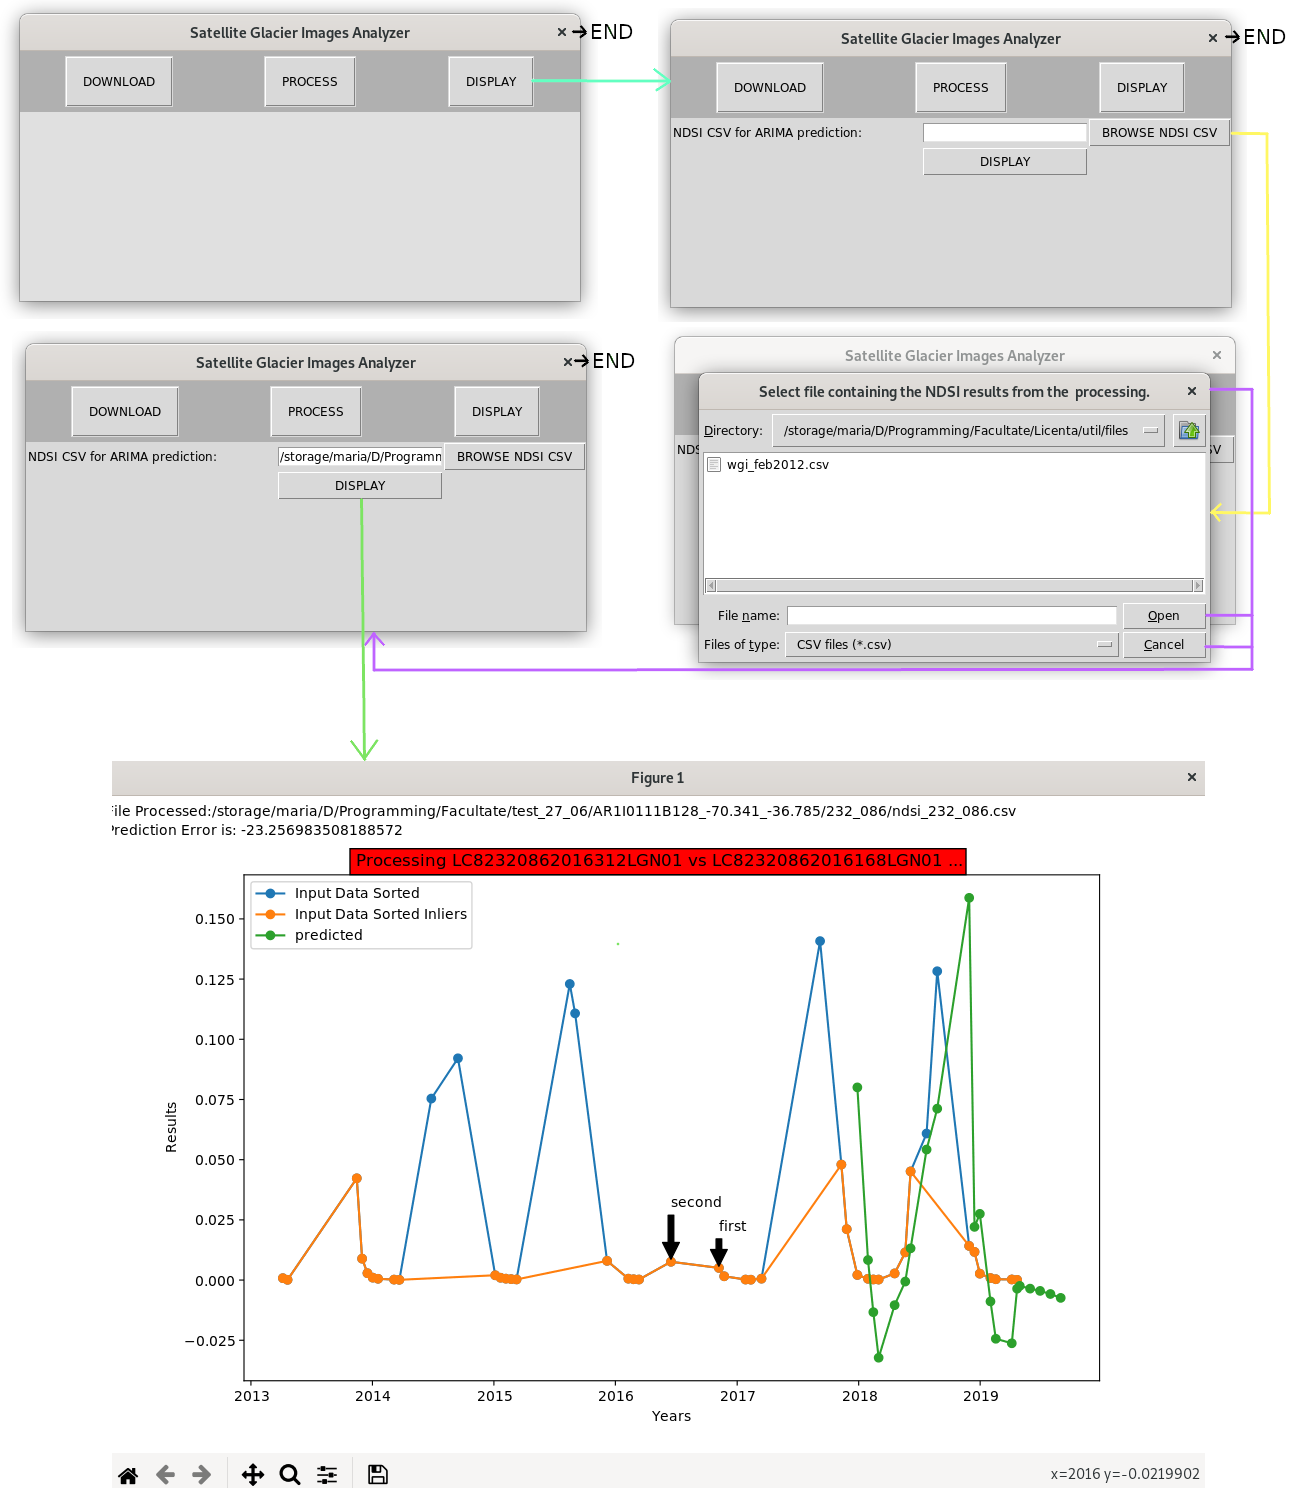
\includegraphics[scale=1.5]{DISPLAY_cmd_gui.png}
		\caption{Display CLI and GUI interactive prediction plot.}
		\label{fig:display_gui}
	\end{figure}
	
	\begin{figure}[H]
		\centering
		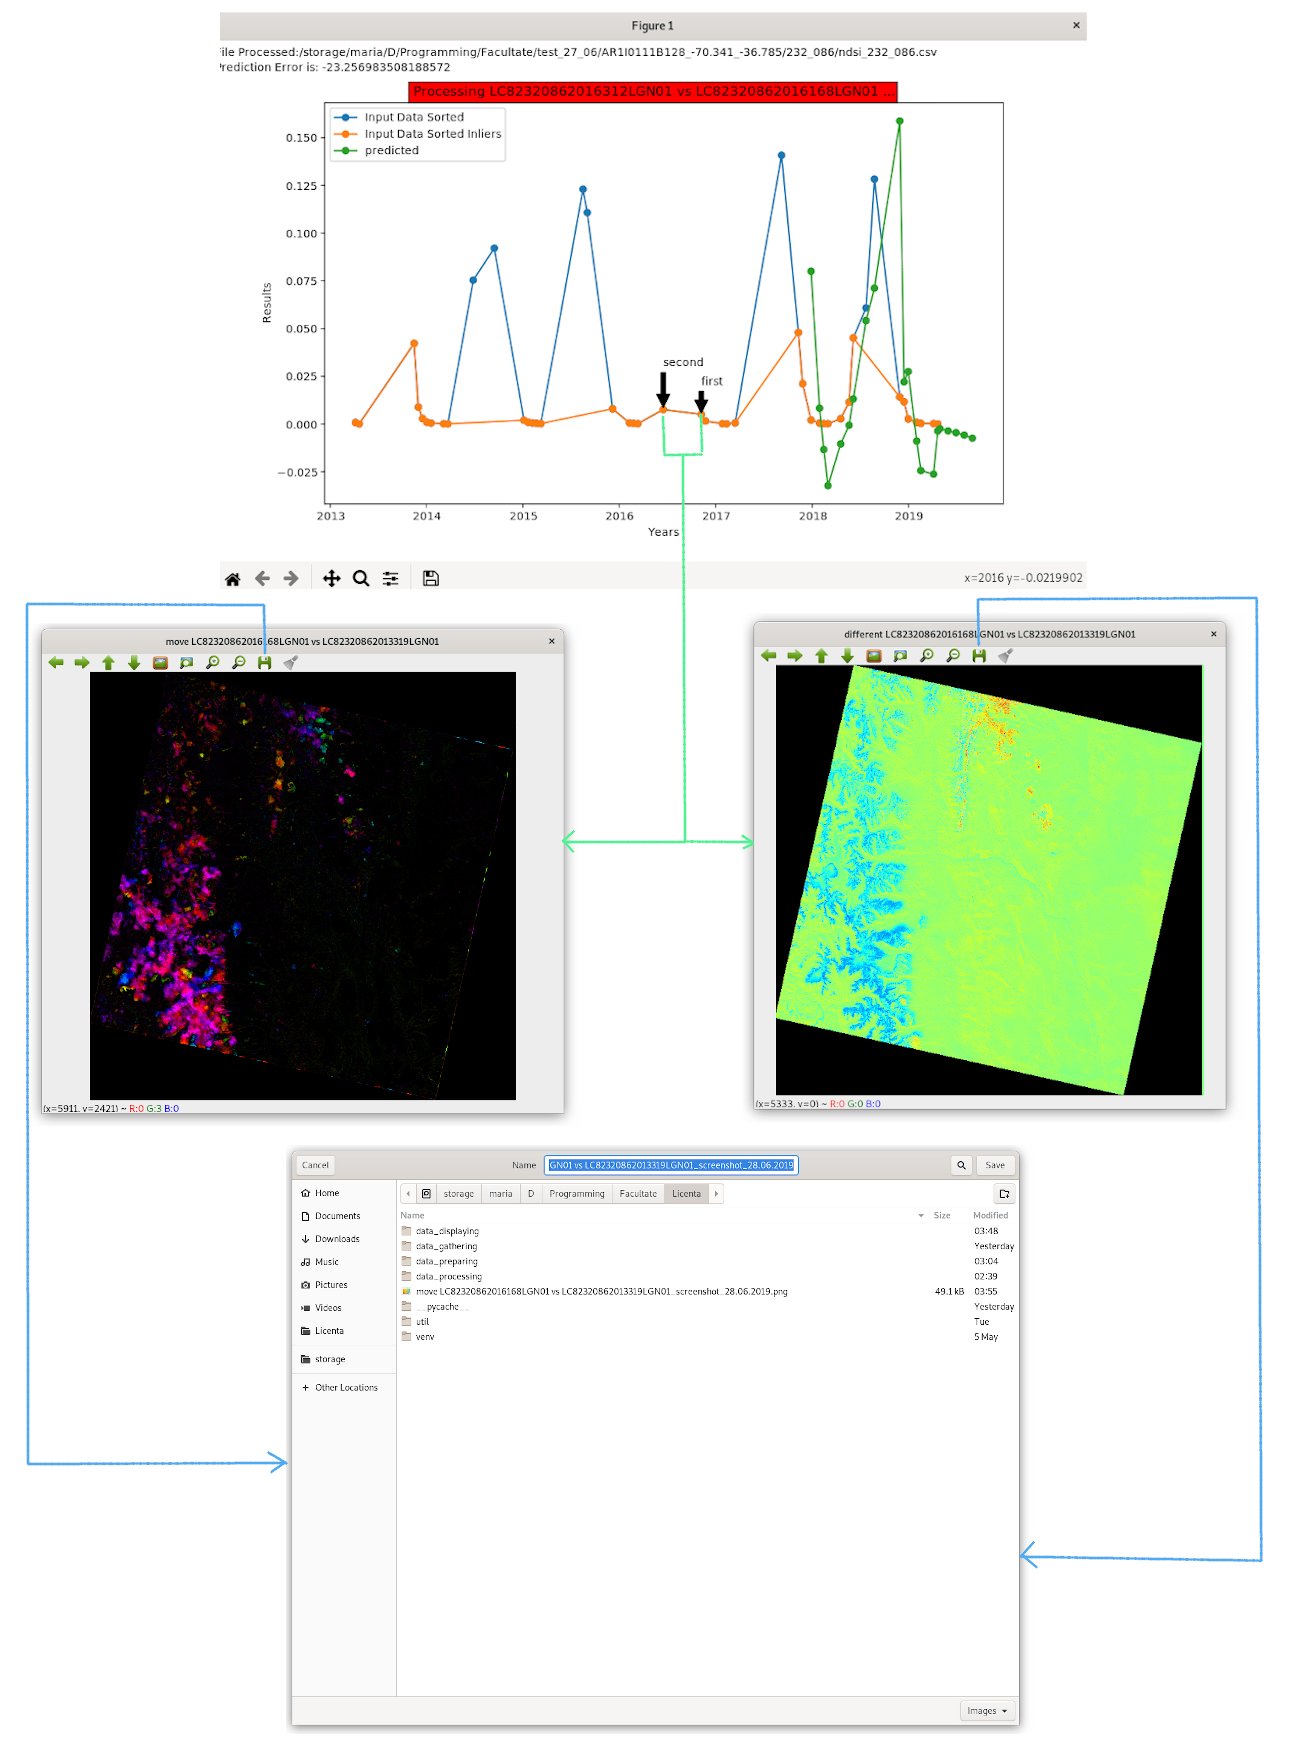
\includegraphics[scale=1.5]{DISPLAY_plot.png}
		\caption{Prediction interactive plot CLI and GUI.}
		\label{fig:prediction_gui}
	\end{figure}

	\section{Main use cases}
	
	The main use case of the application consists of three actions: \textbf{download, process, display, predict}. The use cases of those are the same as described in the user interfaces chapter, while the main use case is the following:
	
	\begin{figure}[H]
		\centering
		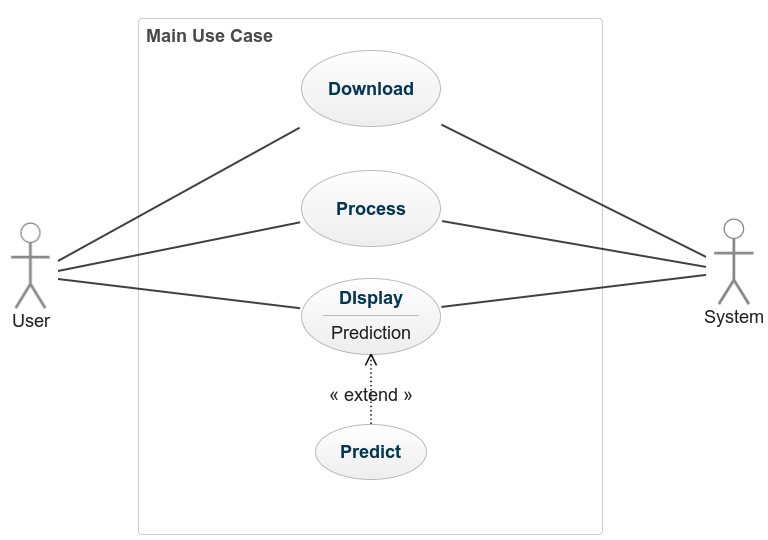
\includegraphics[scale=2]{main_use_case.png}
		\caption{Main use case of the application. The user can choose between downloading, processing or displaying and predicting data. Prediction can only be made if display is chosen, and the interactive plot will pop-up.}
		\label{fig:main_use_case}
	\end{figure}
	
	\newpage{}

	\chapter{Design and implementation}
	
	From the implementation point of view, the application will be described by splitting it into four parts: \textbf{download, process, display, predict}, since the three can be run independently, and each is a main part from the whole. The general view is that the application can search and download images if the user does not have any, which are handled by using the \textbf{sat-search library}; if the user already has a directory with images, the next step is to \textbf{calculate the NDSI} in order to extract the snow pixels from the images, and align them, so that implementing the creation of difference and movement images can be done without discrepancy between pixels, which would result in blurry, incorrect images. The resulting images are written to a directory which the user chooses, along with two csv files, one which holds the results from the NDSI processing (ratio of snow pixels found in each image, along with other information which will be discussed in more detail in the processing section), and an alignment csv, which contains data on how many successful alignment have been created, and the parameters used for achieving such results. The NDSI csv is necessary in order to calculate the prediction on snow coverage for the path and row of a glacier, as well as starting the \textbf{interactive plot which will be used to view the results}, and calculate the difference and movement pictures between two chosen images. 
	
	
	\section{Download}
	The download process is implemented based on \textbf{sat-search}, by using the CLI or GUI, paired with the .csv file which contains information on the glaciers to be searched and downloaded, procured by the user beforehand (either by using Earth Explorer or World Glacier Inventory's searching engines, displayed in Figures 3.1, 3.2 and 3.3). The structure of the .csv file depends on the chosen parameters to download (the process of downloading from the World Glacier Inventory \cite{world_glacier_inventory} is described in the Functional Description chapter). When the user procures the file containing the necessary information for starting the download, it can be used to start searching. The searching, as well as the download, are implemented using \textbf{multiprocessing}, which fastens the waiting time, which is necessary, since it is quite expensive due to the large download file resolution (one .TIF image is between 35 and 65 MB, which makes just one folder of images approximately 1-3 GB, depending on how many images are found.), as well as downloading from the Landsat 8 Archive. Searching returns a \textbf{json search file}, which is passed to download. Since we use multiprocessing to improve the execution time, ensuring that a download process does not start before a search process, the searching was implemented synchronous, while the download is asynchronous, since the speed of download depends on network parameters. The images are downloaded in a folder chosen by the user, having a file hierarchy described in the Functional Application chapter (Figure 3.4). The class diagram of the downloading process is described below: 
	
	\begin{figure}[H]
		\centering
		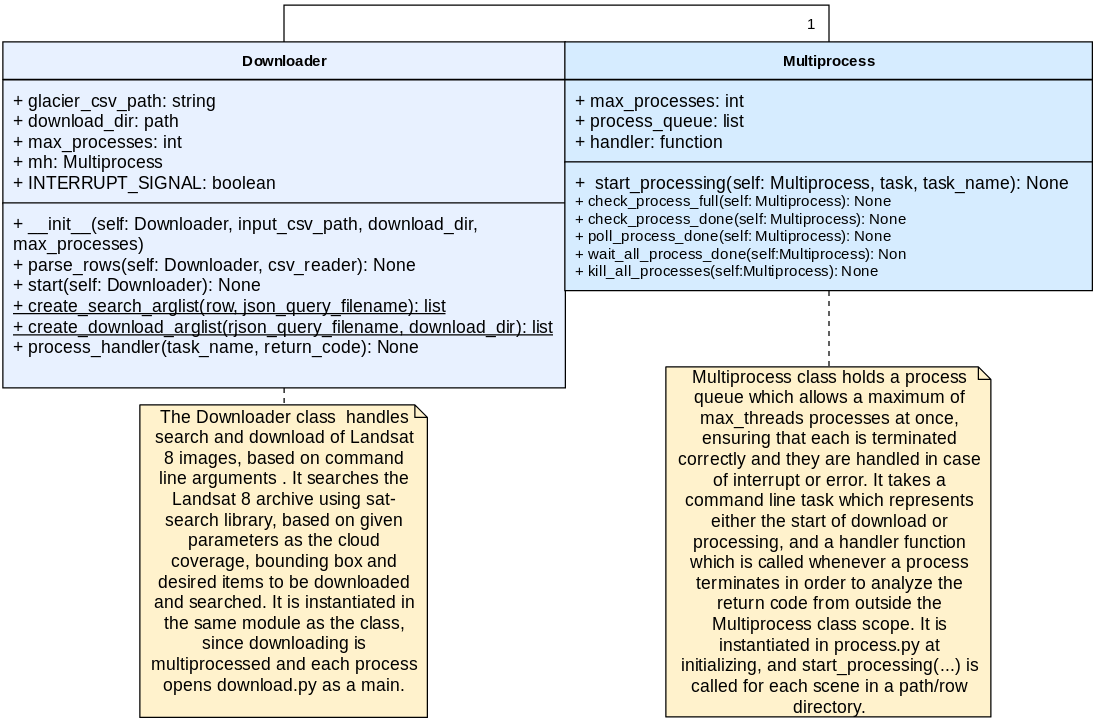
\includegraphics[scale=1.6]{download_process_class.png}
		\caption{Download process class diagram.}
		\label{fig:download_process_class}
	\end{figure}

	\section{Alignment and NDSI}
	
	\subsection{Alignment}
	Accurate alignment of images in a path row folder is required in order to ensure a correct creation of difference and movement pictures (described in Functional Application, Figures 3.12 and 3.13). The \textbf{goal} of this processing part is to achieve results with as little misalignment as possible, meaning distances between pixels with the same coordinates close to 0. Alignment of two images is done by \textbf{collecting features} from each image and trying to \textbf{match them} in order to obtain a list of matches which will be used by the \textbf{warping algorithm} to distort the image on which is applied, such that there is no misalignment between them at the end. 
	\vskip 0.5 cm
	In our case, since the images are almost similar visually, we rely on having a strong \textbf{corner detection algorithm to find edges in mountains} and other geographical features from the images, since they are stable in time and can be reliable as a \textbf{keypoint}. After ensuring that the keypoint detection was successful, we need to calculate the \textbf{descriptors} in order to uniquely identify a small path of data in a huge image (the key-points are found as a circle of 16 pixels in the image which has a resolution of between 7000x700 and 8000x8000). With the key-points assigned to their descriptors, we have to make the ties of features between the two images: since each image has a set of key-points and descriptors, if the algorithm finds that two of the last are equal, that means it found a feature which will be used as a matching line between the reference image and the current one. We need to \textbf{set a limit} on how many key-points are found, as well as how many matches are considered good. In our case, the best results were by considering \textbf{5000 key-points} with \textbf{25\%} of the \textbf{matches} considered good (taken by top). The next step after trimming the bad matches out is to calculate a \textbf{warp matrix} in order to distort the image such by doing that, there will be no misalignment, or as one as close to 0, between the pixels of the reference image and the ones from the image which we apply the warp on. 
	\vskip 0.2cm
	In order to achieve such results between two images, we used the following computer vision intelligent algorithms:
	\begin{itemize}
		\item \textbf{Oriented FAST and Rotated BRIEF (ORB)} \cite{orb_1};
		\item \textbf{Harris corner measure} \cite{harris_1};
		\item \textbf{Random Sample Consensus (RANSAC)} \cite{ransac_1}.
	\end{itemize}
	
	ORB is a fusion of \textbf{Features from accelerated segment test (FAST) keypoint detector  \cite{fast_1} and Binary Robust Independent Elementary Features (BRIEF) descriptor}  \cite{brief_1} with many modifications to enhance the performance. First it use FAST to find key-points, but its corner detection is not performant enough, failing to find enough good results; Since we need powerful corner detection on mountain features, we paired up ORB's key-point and descriptor detection with \textbf{Harris corner measure \cite{harris_1} to find top 25\% points among them}, which also uses pyramid to produce multiscale-features for large files. \cite{orb_1}. 
	\vskip 0.2cm
	After creating the matches, we use the \textbf{RANSAC} algorithm create the \textbf{warping}. RANSAC is an iterative method to estimate parameters of a mathematical model from a set of observed data that contains outliers, when outliers are to be accorded no influence on the values of the estimates \cite{ransac_2}. We chose this we know that between our images there is an \textbf{affine transformation} (translated, rotated, scaled), and this technique helps filter out bad matches only leaving the ones that satisfy the motion model between two images. 
	
	By using this starting point, the following \textbf{improvements} were applied in order to get to a \textbf{correct alignment percent} of almost \textbf{98\%} for approximately \textbf{85\% files in a path row folder}:
	\begin{enumerate}
		\item \textbf{Two feature sets}: taking features from the \textbf{reference and current image} (green or swir1);
		\item \textbf{Box split}: splitting the two images in \textbf{8 boxes} and taking keypoints and descriptors from each;
		\item \textbf{Prune matches}: splitting the two images in 8 boxes and taking features from each, while also \textbf{pruning the matches} which were not almost straigH;
		\item \textbf{Three feature sets}: Taking features from the \textbf{reference and both green and swir1 matching bands}, while also splitting them in 8 boxes and taking keypoints and descriptors from each and applying pruning of matches.
	\end{enumerate}
	
	\paragraph{1. Two feature sets} When aligning the images, there are two cases: either we align a \textbf{green band} or a \textbf{swir1 band}. By analyzing the results of this approach on \textbf{237} glaciers, we observed that the \textbf{mean value of ratio successful alignments} on a path row directory was \textbf{0.054868}. An example of a match result and align result using this approach is displayed below:
	
	\begin{figure}[H]
		\centering
		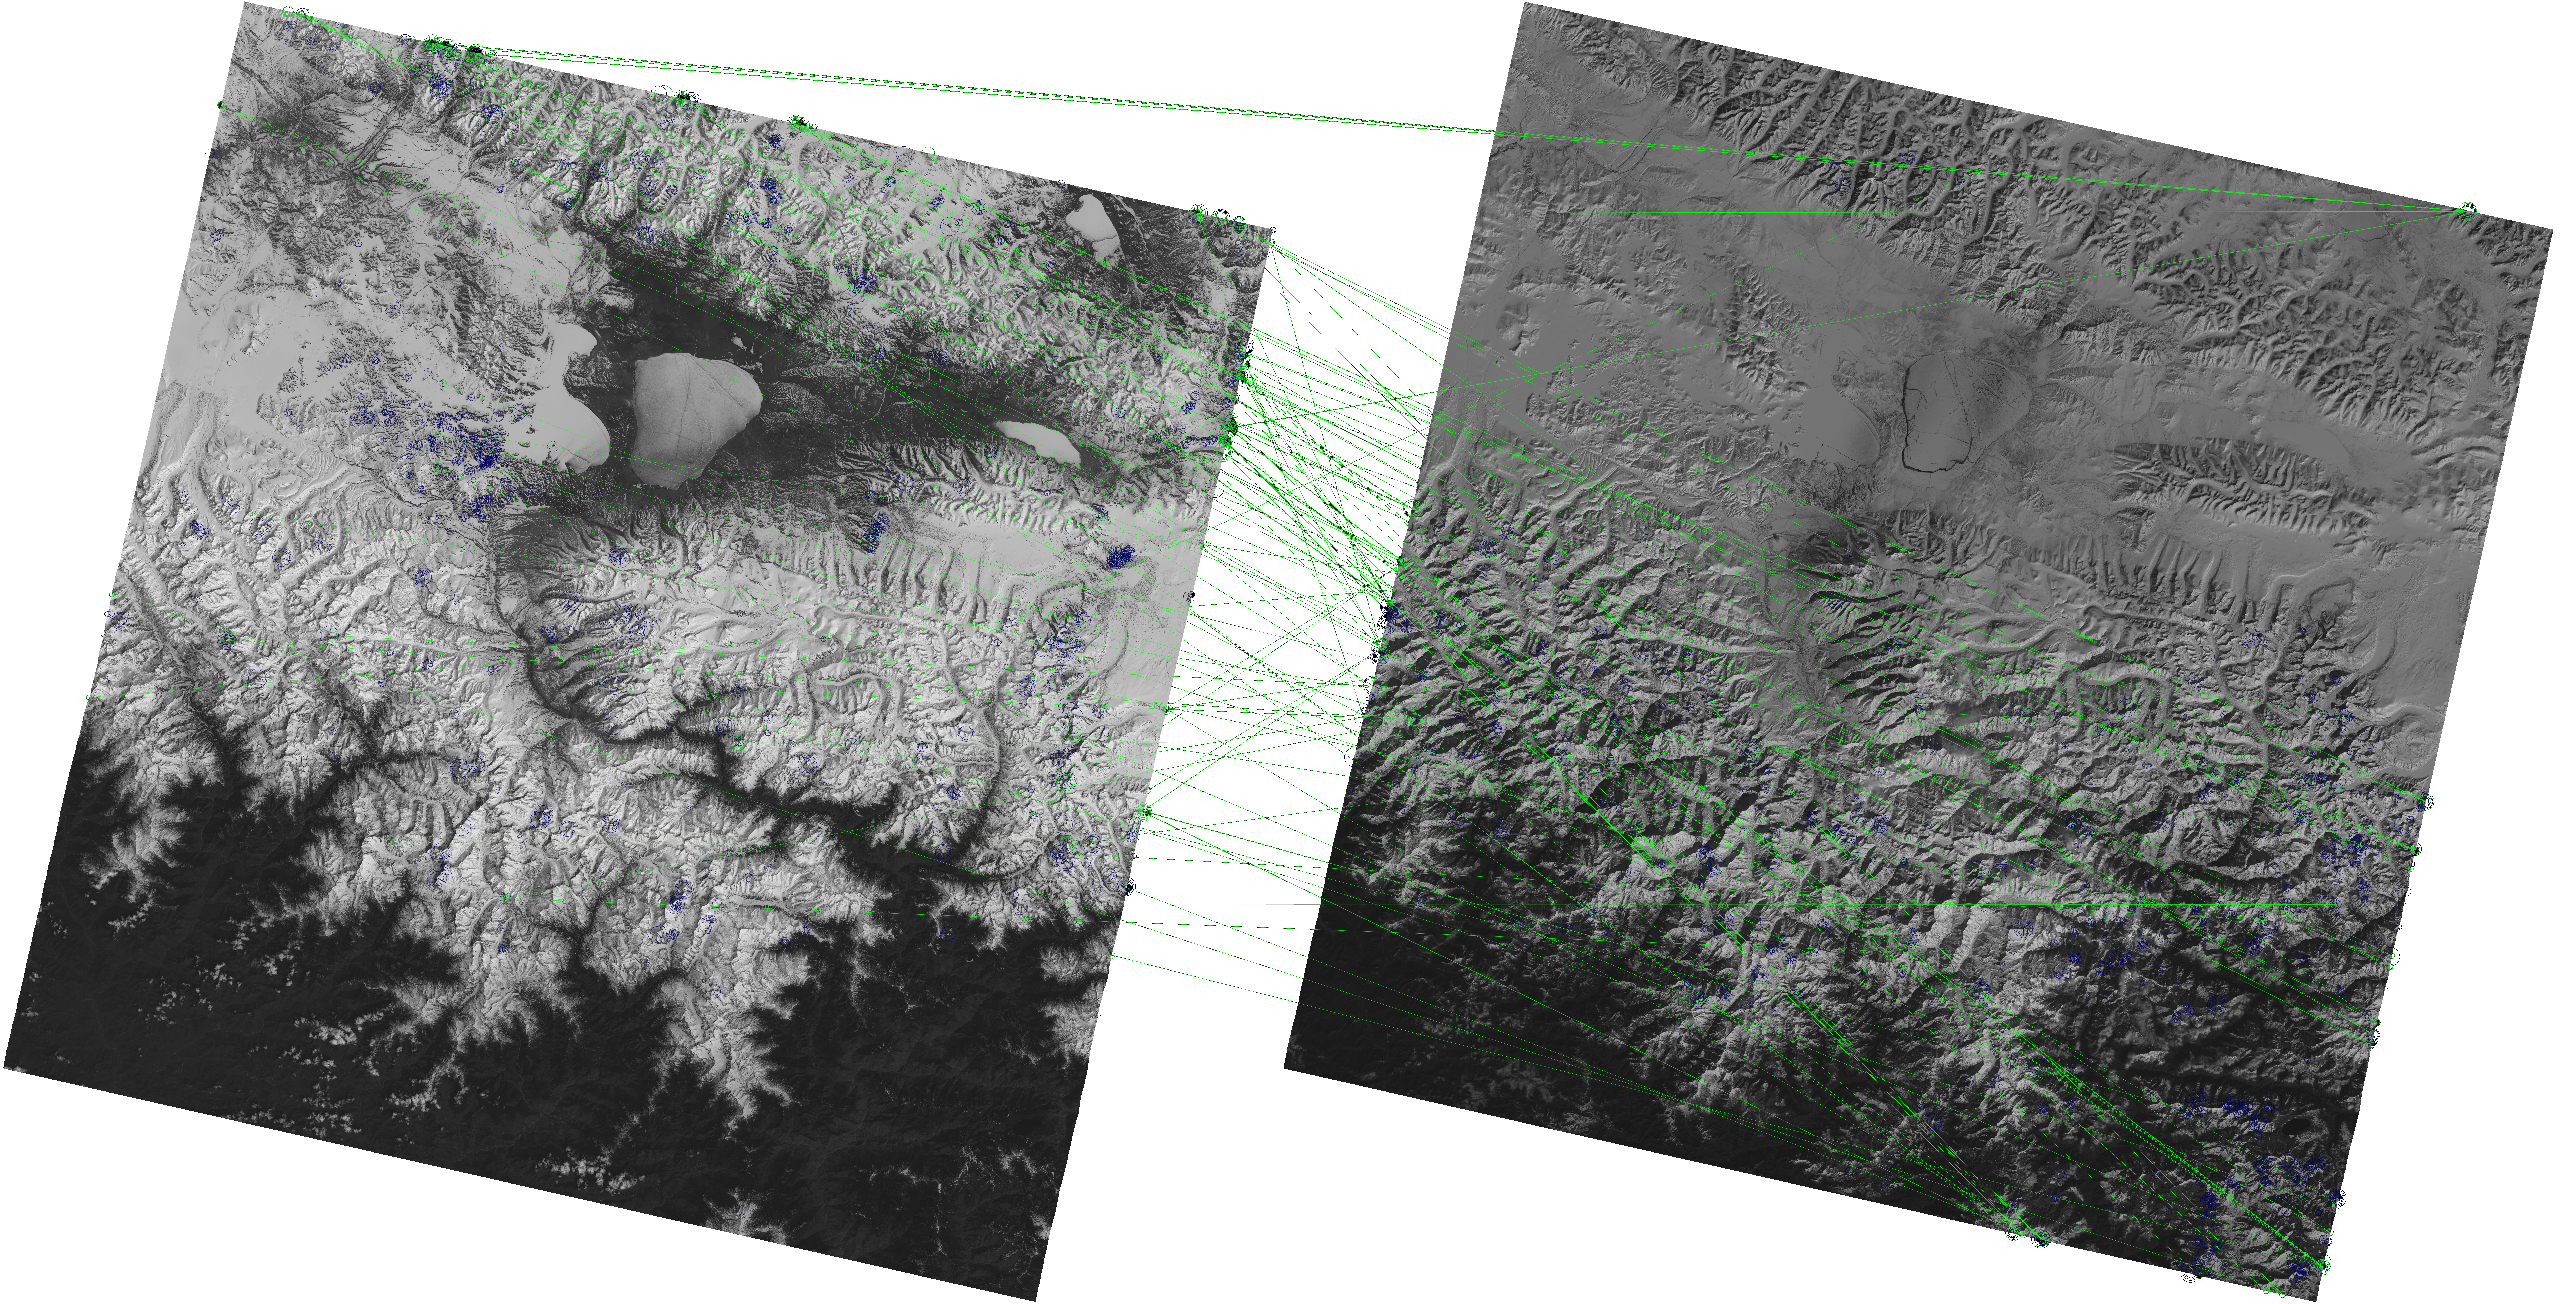
\includegraphics[scale=0.25]{bad_matches_1.png}
		\caption{Matches between the reference image (left, green) and image to be aligned (rigH, SWIR1).}
		\label{fig:bad_matches_1}
	\end{figure}
	
	\begin{figure}[H]
		\centering
		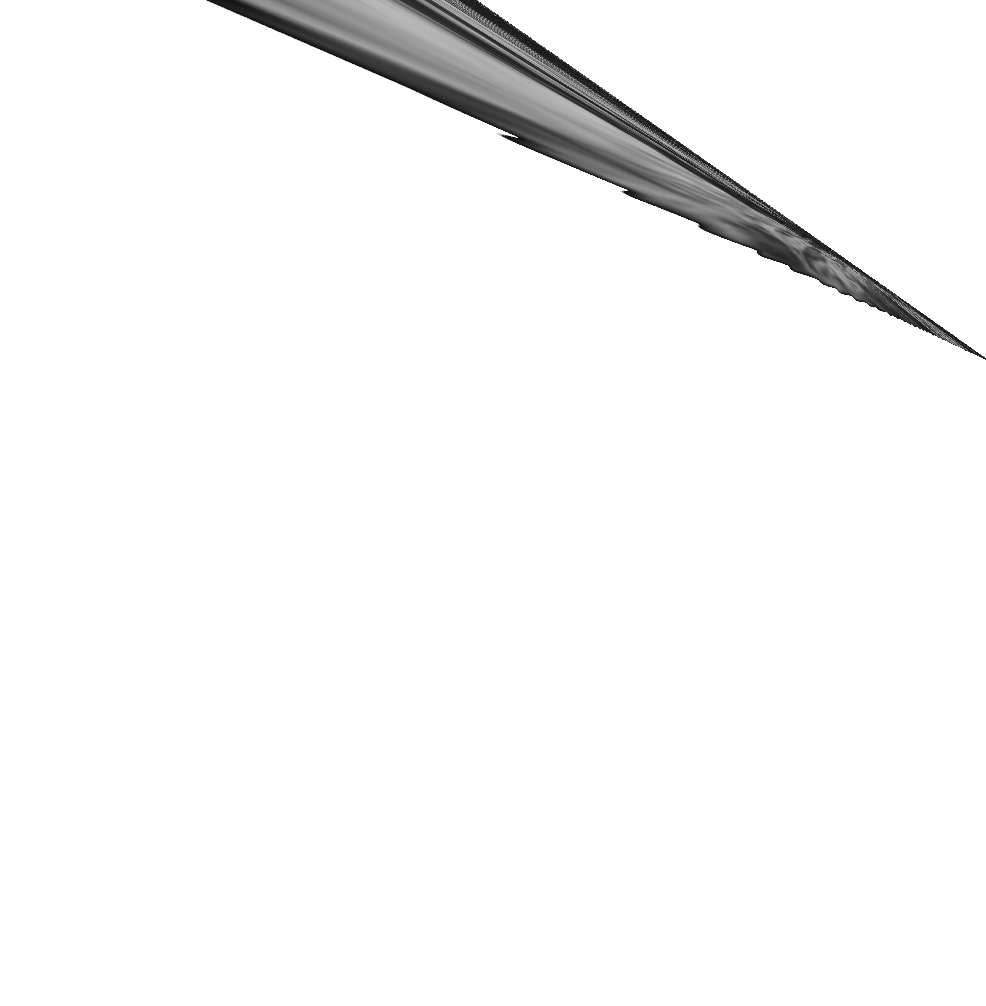
\includegraphics[scale=0.1]{bad_result_1.png}
		\caption{Image after warping the affine matrix on the SWIR1 band.}
		\label{fig:bad_reference_1}
	\end{figure}
	
	\paragraph{2. Box split} An improvement to the first approach was to \textbf{split the images into 8 boxes}, and apply ORB and Harris on each box; This step was needed because in most of the results, features were only found on a box of 25\% of the image, which completely unbalances the affine matrix calculation. By this approach, we were able to find much better results, on the same \textbf{237} glaciers, we observed that the \textbf{mean value of successful alignments} on a path row directory was \textbf{0.3854}, which means an \textbf{improvement} with \textbf{0.330532}.
	
	\begin{figure}[H]
		\centering
		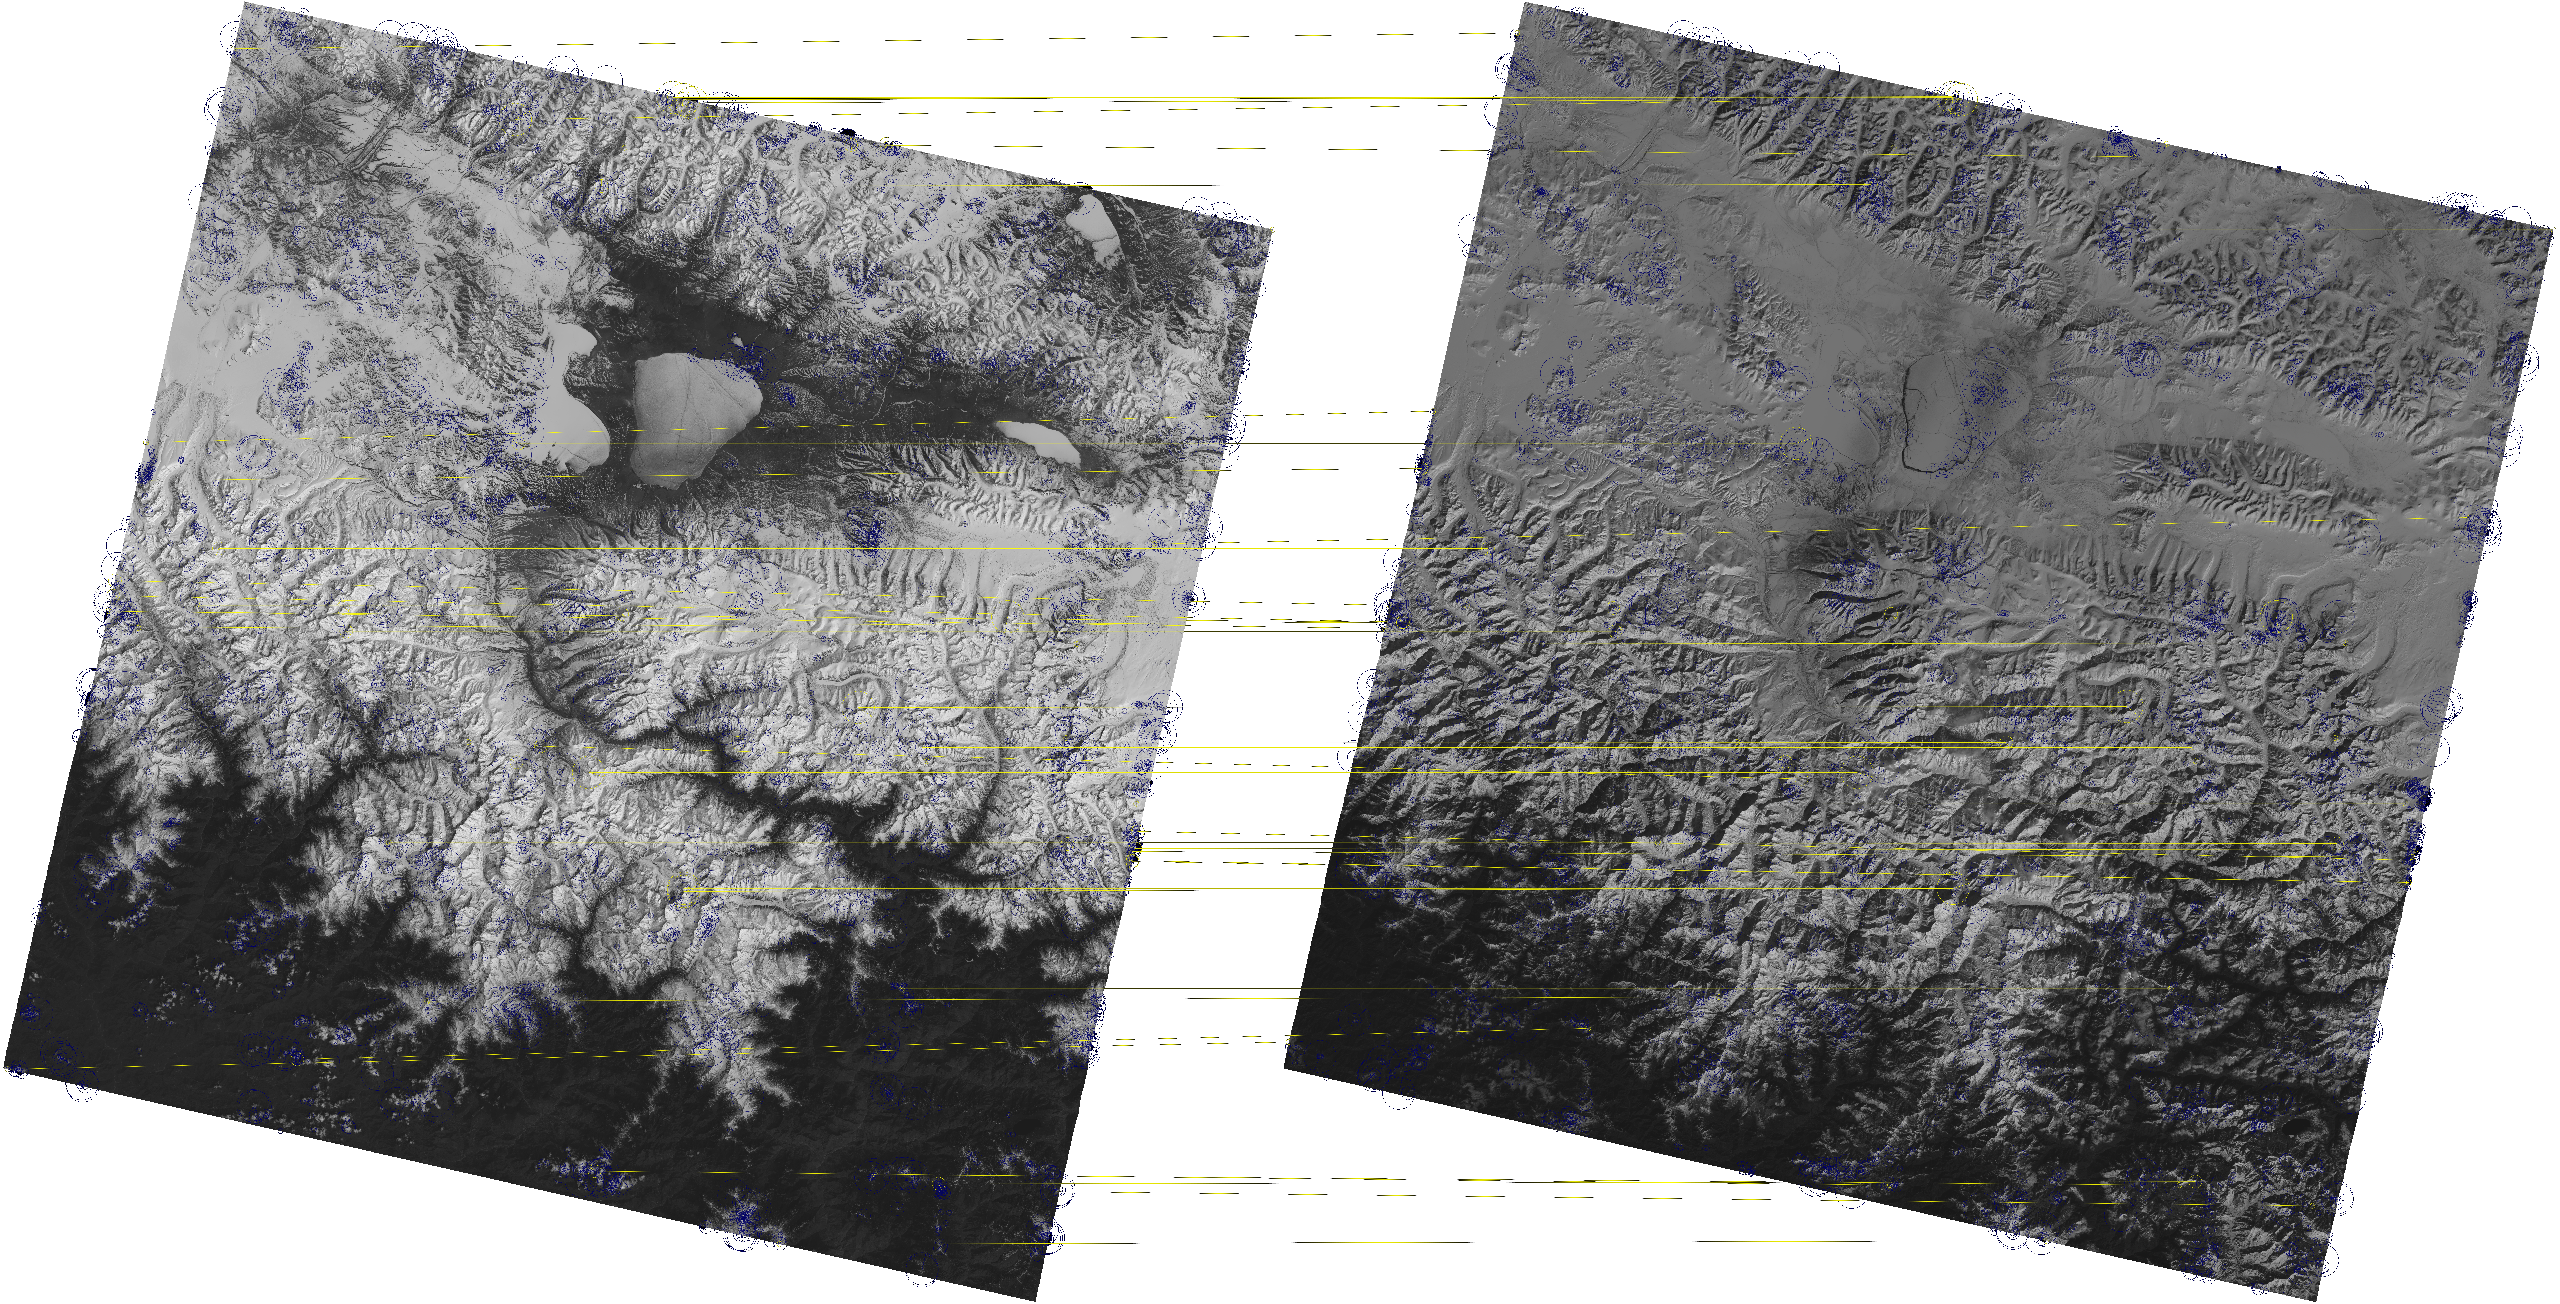
\includegraphics[scale=0.25]{matches_2.png}
		\caption{Matches between the reference image (left, green) and image to be aligned (right, SWIR1), after box feature find.}
		\label{fig:bad_reference_1}
	\end{figure}
	
	\paragraph{3. Prune matches} Even if the last approach gave better results, the ratio could be brought up, by \textbf{pruning the bad matches}. Since the Landsat 8 satellite could not have errors of more than approximately 200 pixels, any match which has a point discrepancy of \textbf{more than 200 pixels} on the xy axis represents a \textbf{bad descriptors match}, and therefore should not be taken into consideration.  By this feature, we were able to find result with a mean of \textbf{0.733}, on the same \textbf{237} glaciers, which means an \textbf{improvement} with \textbf{0.3476}. The following example of before and after prune match is displayed below:
	
	\begin{figure}[H]
		\centering
		\includegraphics[scale=0.25]{matches_before_prune.png}
		\caption{Matches between the reference image (left, green) and image to be aligned (right, SWIR1), before prune matches improvement.}
		\label{fig:bad_matches_2}
	\end{figure}
	
	\begin{figure}[H]
		\centering
		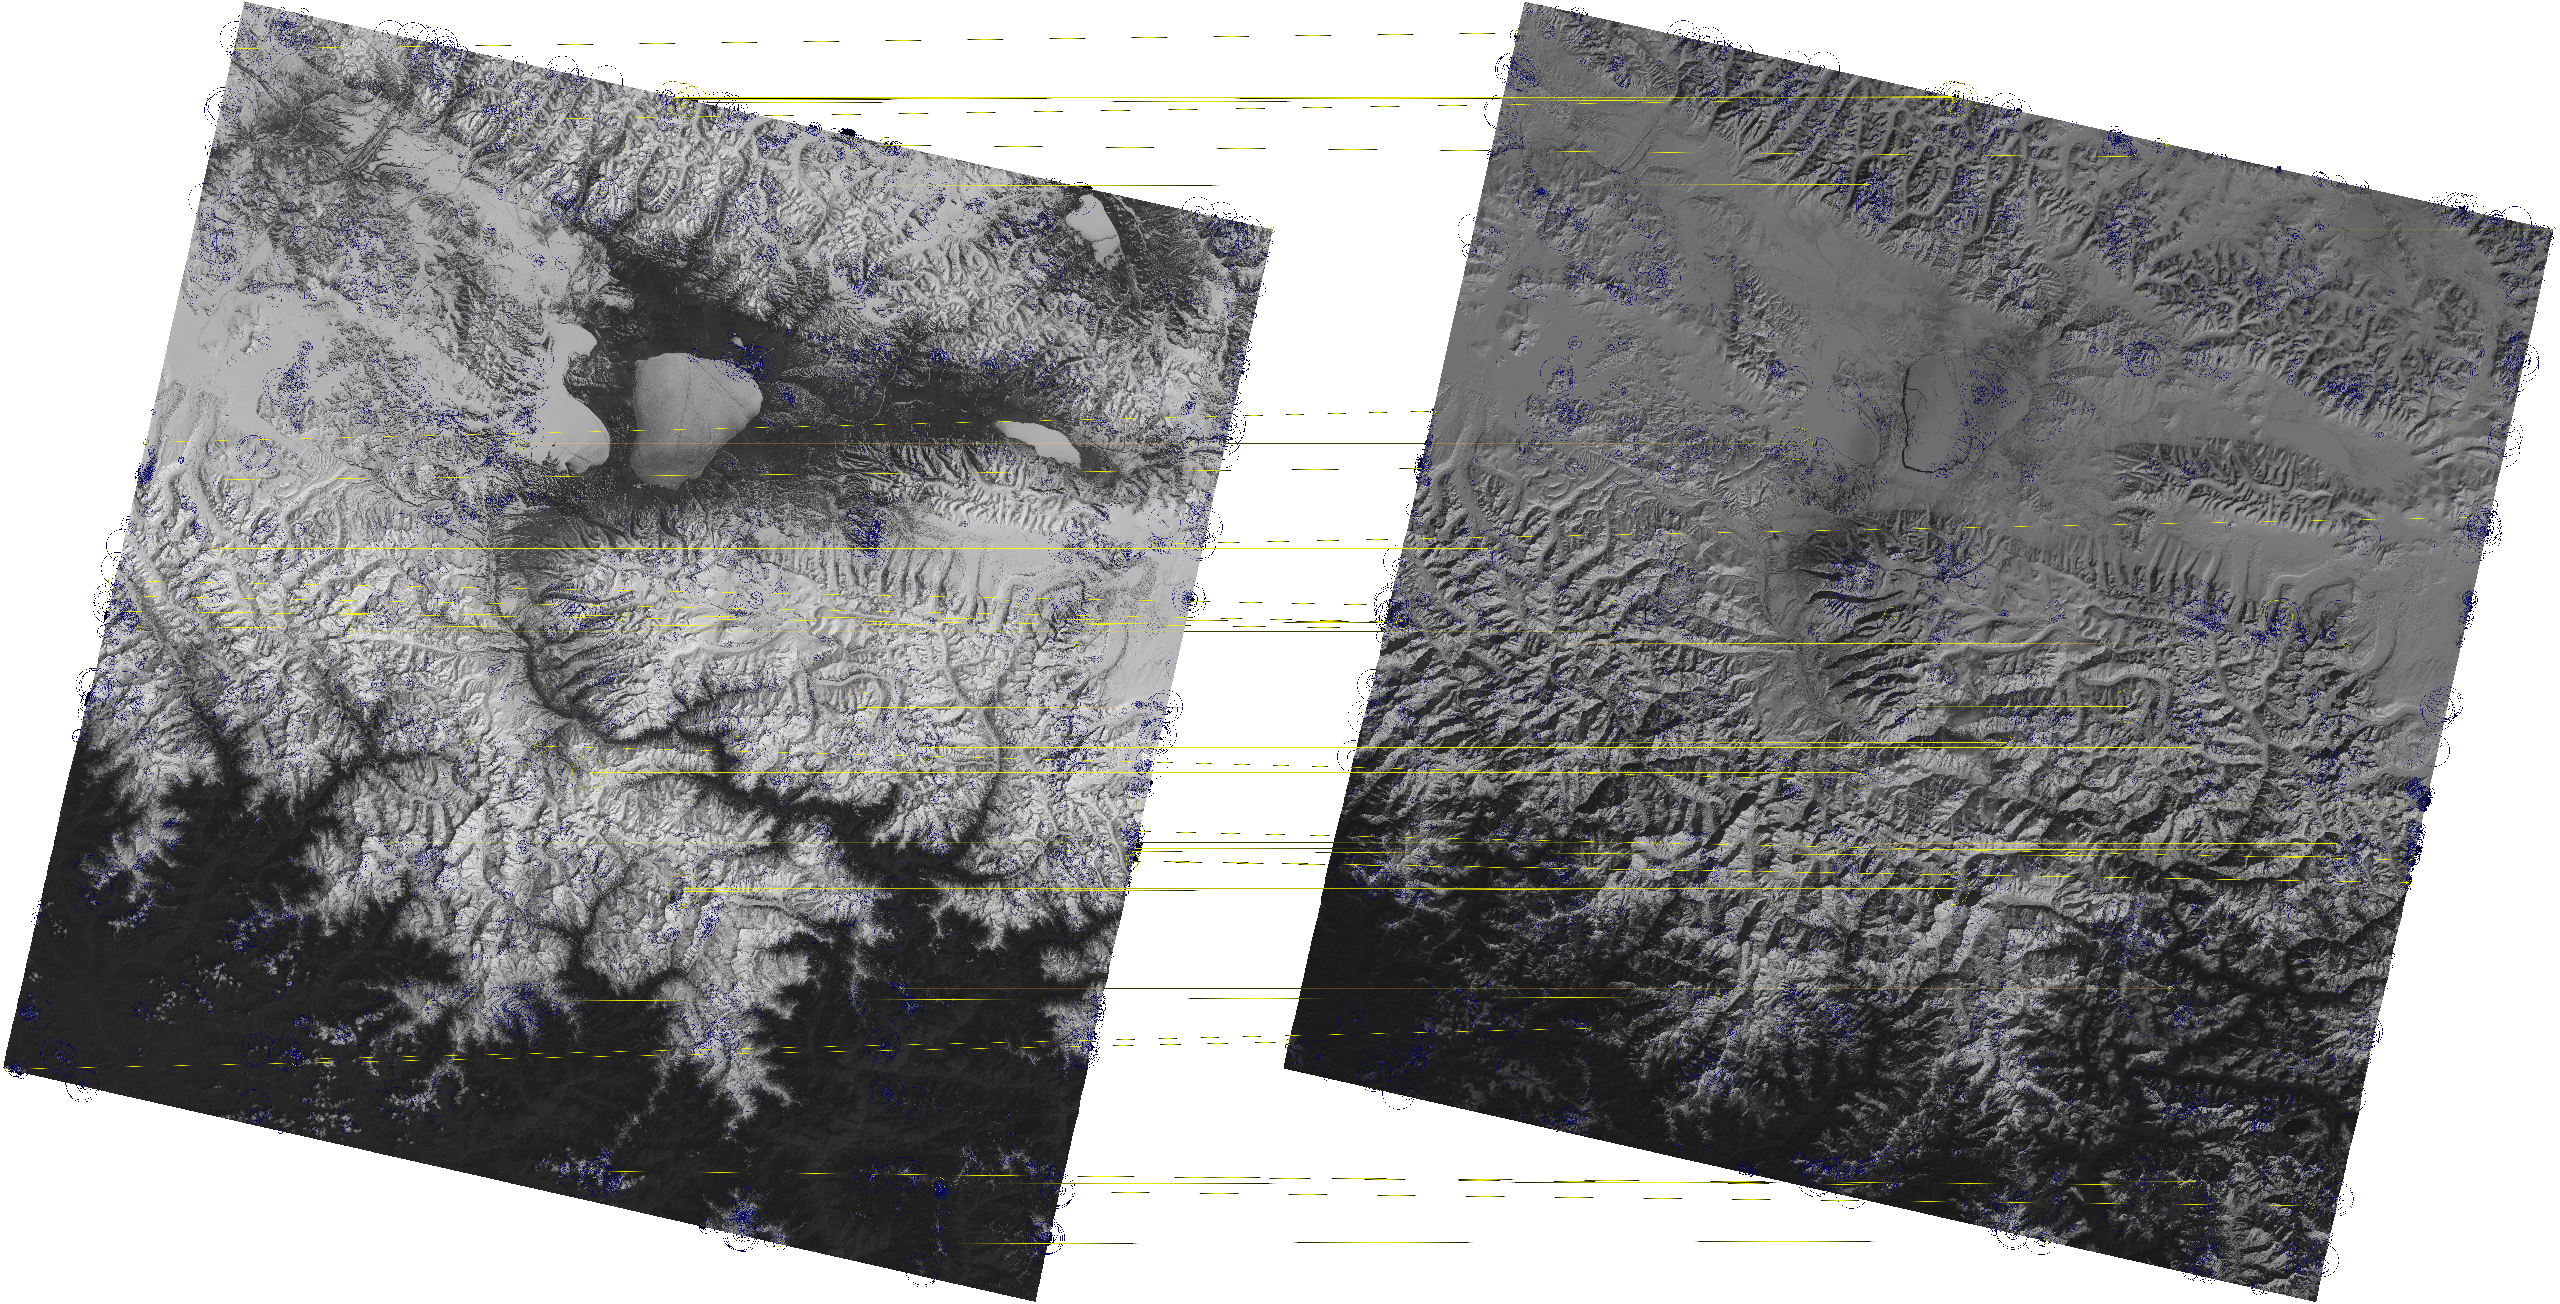
\includegraphics[scale=0.25]{matches_after_prune.png}
		\caption{Matches between the reference image (left, green) and image to be aligned (right, SWIR1), after prune matches improvement.}
		\label{fig:bad_matches_3}
	\end{figure}
	
	\paragraph{4. Three feature sets} Finally, the improvement which achieved a ratio of successful alignments over total trials of \textbf{0.896} was gathering features not only from the reference image and the current green or SWIR1 one, rather both, since they are already aligned between each other. The Landsat 8 has pixel discrepancy between different scenes, but all the bands are aligned. By taking key-points from the reference, current band and its pair, we were able to achieve an improvement which is more than enough in producing aligned images (NDSI, green and SWIR1). The following image is the result of the \textbf{alignment using all the four features}.
	
	\begin{figure}[H]
		\centering
		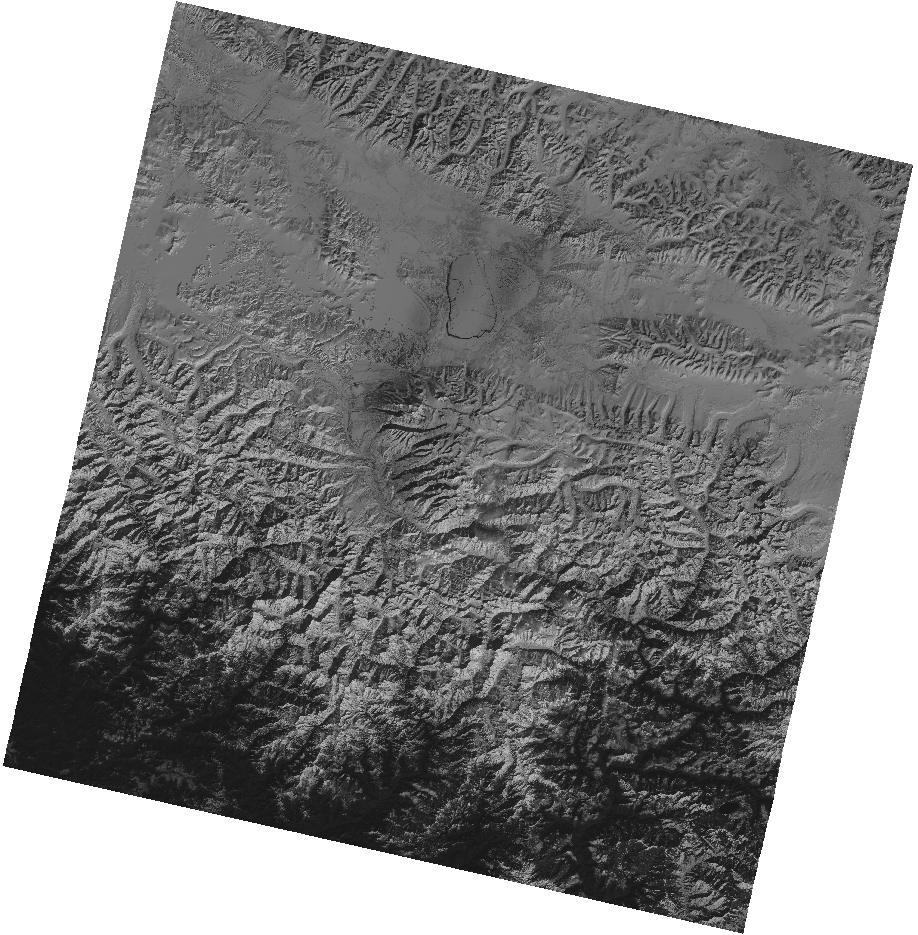
\includegraphics[scale=0.3]{matches_3.png}
		\caption{The aligned image after applying all four features.}
		\label{fig:bad_matches_3}
	\end{figure}
	
	\subsection{NDSI}
	
	The NDSI is calculated as described in the Functional Decription, by reading the \textbf{image as a numpy array}, and applying the formula 
	\[ndsi = \frac{green - swir1}{green + swir1}    \cite{ndsi_2}\]
	on the n-dimensional arrays. A \textbf{threshold of 0.5} is used for distinguishing between snow and other objects in the image. The NDSI is calculated for each pair of green and SWIR1 images along with alignment, such that when alignment is started, the NDSI is already created and can be included in the \textbf{scene with NDSI} image (NumpySceneWithNdsi class). The \textbf{snow ratio} of the image is introduced in the \textbf{NDSI csv} for \textbf{construction of the prediction data set}. The NDSI has the class diagram displayed in Figure 4.8. 
	\vskip 0.2cm
	
	\begin{figure}[H]
		\centering
		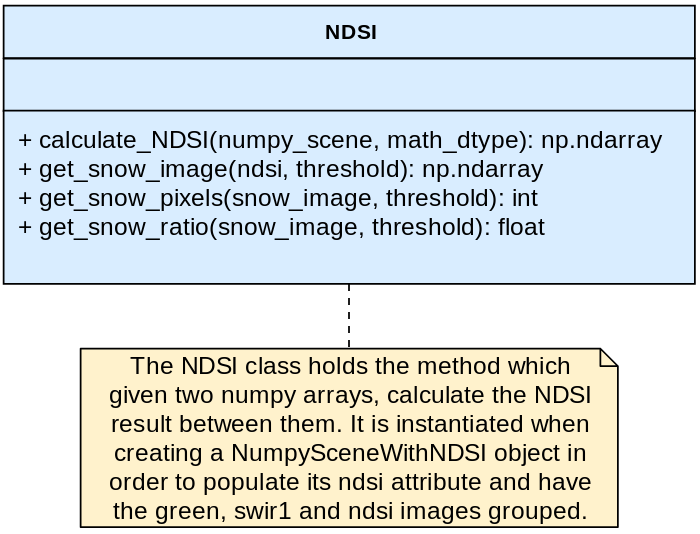
\includegraphics[scale=1.7]{ndsi_class.png}
		\caption{The NDSI class diagram..}
		\label{fig:ndsi_class}
	\end{figure}

	
	The alignment and NDSI processing is done by the \textbf{ProcessImage class}, which binds the two processes together in order to achieve the goal of creating a path and row folder of aligned scenes with computed NDSI. The processing including NDSI and AlignORB has the following class diagram, as shown in Figure 4.9.

	
	\begin{figure}[H]
		\centering
		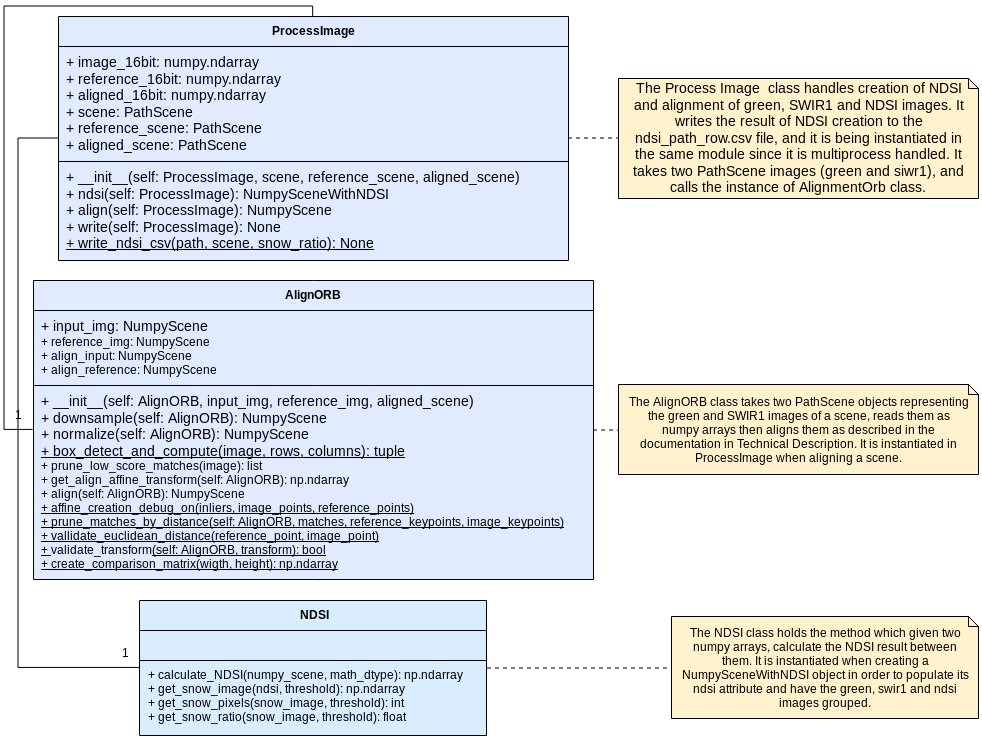
\includegraphics[scale=2.1]{process_image_class.png}
		\caption{The alignment and NDSI processing for a path and row directory class diagram.}
		\label{fig:process_align_ndsi}
	\end{figure}

	\newpage{}
	
	\section{Display and ARIMA prediction}
	
	\subsection{Data set normalization}
	
	The display process handles creating the plot for \textbf{data set prediction and creation of difference and movement images}. When calling the display process, the \textbf{ndsi\_path\_row.csv} file is analyzed using the data set handler module (class DatasetHandler) as:
	\begin{itemize}
		\item \textbf{Sorting the data set entries such that the images are in chronological order.}
		\item \textbf{Detecting and removing outliers from the data set.}
	\end{itemize}
	After the data set has been normalized, it is ready to be redirected to \textbf{plotting and predicting}.
	
	\subsection{Data set plotting}
	
	The normalized set of snow ratios resulted from the NDSI process is displayed in an interactive plot created with \textbf{matplotlib} library, as:
	
	\begin{figure}[H]
		\centering
		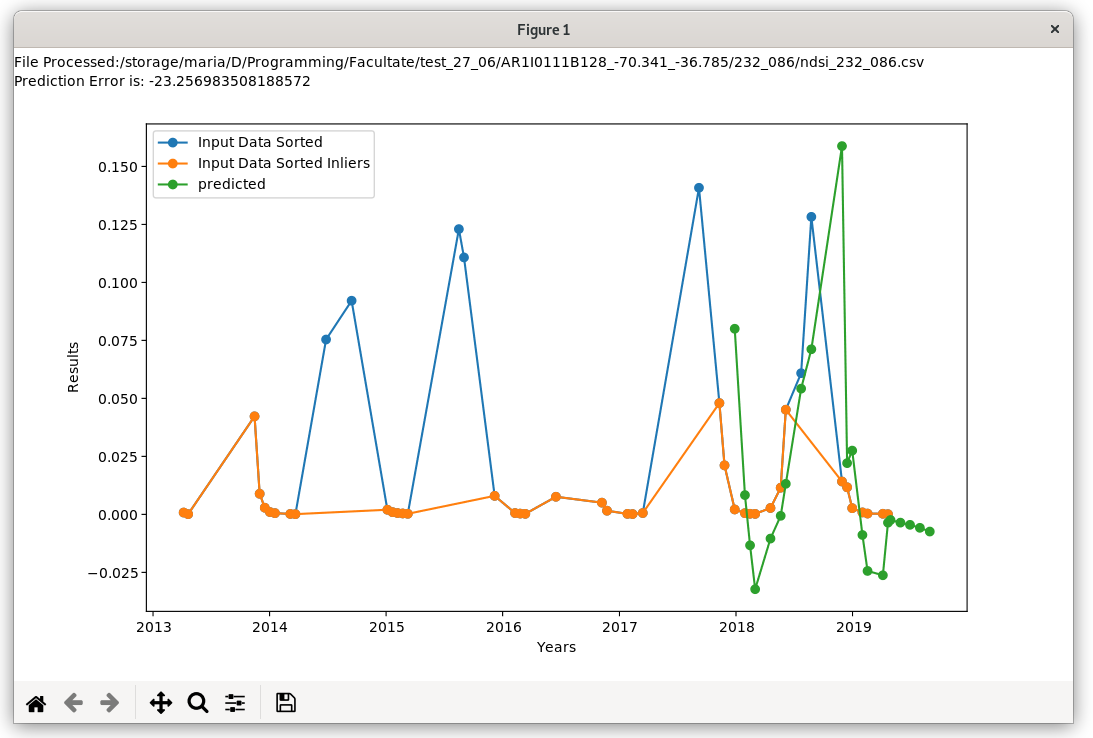
\includegraphics[scale=1.5]{plot_1.png}
		\caption{Plot of glacier AR1I0111B128, with coordinates(-70.341, -36.785), on path and row 232, 086.}
		\label{fig:plot_1}
	\end{figure}
	
	\subsection{Data set predicting}
	
	We used the ARIMA predicting algorithm with (4, 2 and 0) parameters \cite{arima_parameters} by splitting the data set into \textbf{66\% train} and \textbf{33\% test}, in order to give ARIMA a view over the data set and ensuring that the prediction is as accurate as possible, with a \textbf{small mean error}. We ensured that the prediction object matches the good position one by finding the nearest neighbor so the error is calculated both on x and y axes (time and snow ratio). 
	\textbf{The mean error} is calculated by summing up the differences between the prediction and its nearest neighbor measurement, then divided by the total number of predictions and the max value of the snow ratio index. The \textbf{maximum value} is used instead of the nearest neighbor value because the \textbf{discrepancy between objects is very small}, close to zero, which \textbf{leads to artificially high errors}.
	
	\[ ERROR = \frac{d_{1} + d_{2} + ... + d_{n}}{N * MAX} \] 
	
	\begin{table} [H]
		\center
		\begin{tabular} {|  l | L{10cm} |}
			\hline
			ERROR & Error between the prediction and the actual value of the snow ratio. \\ [0.2ex]
			\hline
			$d_{1}, d_{2}, ..., d_{n}$ & Differences between predictions and nearest neighbor measurement.\\ [0.2ex]
			\hline
			N & Total number of predictions. \\ [0.2ex]
			\hline
			MAX & The maximum snow ratio value. \\ [0.2ex]
			\hline
		\end{tabular}
		\caption{Prediction error formula.}
		\label{table:ndsi_table}
	\end{table}
	
	For the example in Figure 4.10, the \textbf{mean error is 23}, which means that the prediction was has an error percent of 23\%.
	
	\subsection{Difference and Movement images}
	The interactive plot created in matplotlib \textbf{generates the difference and movement images between two picked plot items}.The date of the scene corresponding to the x axis is searched for in the ndsi\_path\_row.csv file, which is used to find the NDSI images on which the difference and movement will be made. The following figure exemplifies picking of first and second images for this calculation:
	
	\begin{figure}[H]
		\centering
		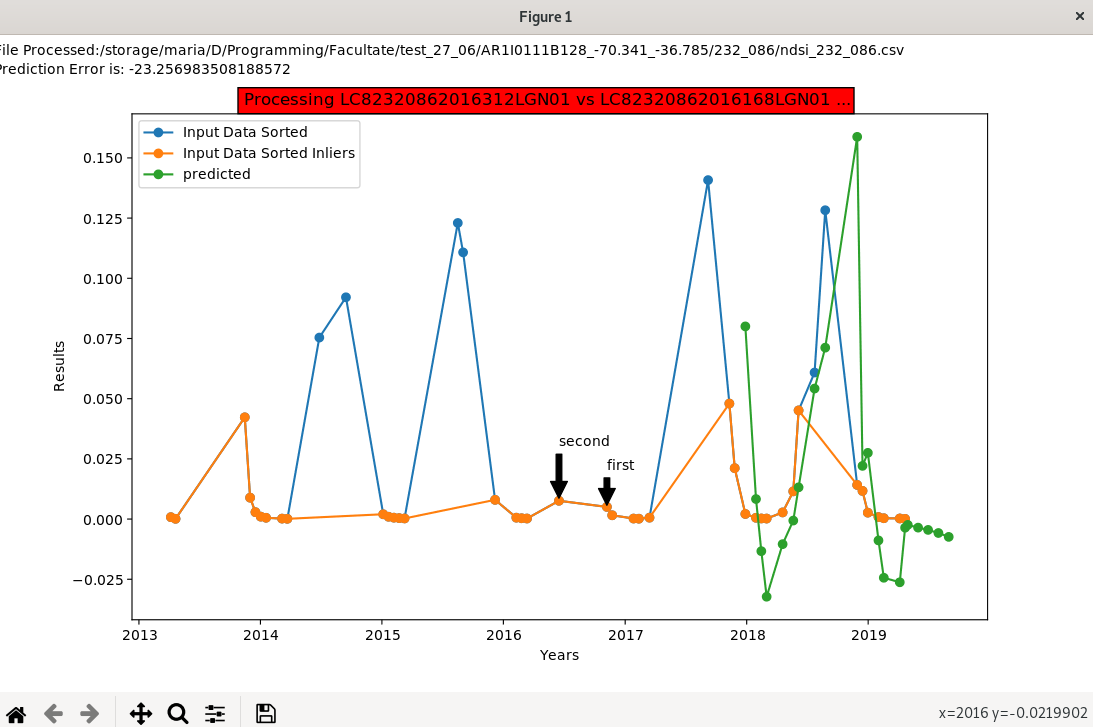
\includegraphics[scale=1.7]{plot_first_second.png}
		\caption{Picking two NDSI images to create their difference and movement images.}
		\label{fig:first_second_1}
	\end{figure}
	
	When the two items are \textbf{picked}, an \textbf{asynchronous process} calling the difference movement module with the name of the scenes, their paths and the output directory for image writing. 
	
	\paragraph{Difference}
	The difference image is calculated by making a \textbf{subtraction} between the two numpy images, therefore highlighting whether snow has appeared or disappeared in comparison to the first picture. 
	
	\paragraph{Movement}
	The movement image is implemented by using the \textbf{Optical flow algorithm}, which is the pattern of apparent motion of image objects between two consecutive frames caused by the movement of object. It is a \textbf{2D vector field} where each vector is a displacement vector showing the movement of points from first frame to second. \cite{optical_flow} We use the algorithm in our image viewing because it works with assuming that:
	\begin{itemize}
		\item The \textbf{intensities} of the pixels do not change by much \cite{optical_flow};
		\item The \textbf{neighbors} of the pixels show the same movement pattern \cite{optical_flow}.
	\end{itemize}
	
	Figure 4.12 shows the results of processing the first and second picked images from the plot.
	
	\begin{figure}[H]
		\minipage{0.48\textwidth}
		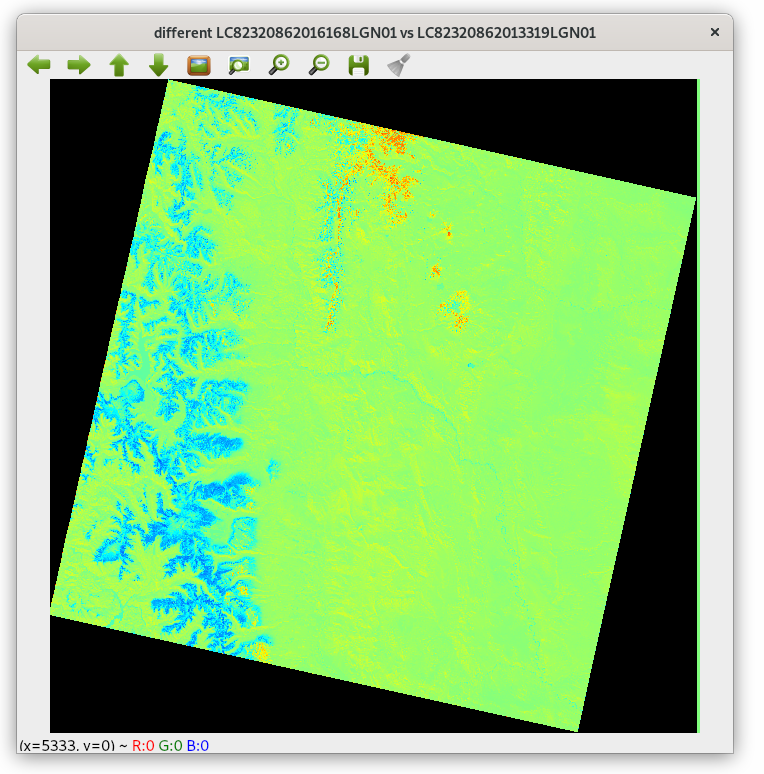
\includegraphics[width=\linewidth]{difference_plot.png}
		\endminipage\hfill
		\minipage{0.48\textwidth}
		\includegraphics[width=\linewidth]{movement_plot.png}
		\endminipage\hfill
		\caption{The difference and movement images for the selected points on the plot.}\label{fig:difference_movement_gui}
	\end{figure}
	
	The results can be \textbf{saved} to disk by pressing the save button in the OpenCV GUI. 
	
	\newpage{}
	\chapter{Performance Evaluation} 
	The first test area is located in Las Heras Department, Provincia Mendoza, Argentina, on the glacier with id AR1J11132208 (-32.272, -69.606), on path 233, row 82. The location has \textbf{50} pictures dating from 2013 to present, with 8 outliers. The estimation on already existing data set had an error of \textbf{21.50\%}, while the extra 10 future estimates keep their direction of approaching 0.
	
	\begin{figure}[H]
		\centering
		\includegraphics[scale=0.5]{21.png}
		\caption{Las Heras Department, Provincia Mendoza, Argentina (AR1J11132208, 233, 82).}
		\label{fig:first}
	\end{figure}
	
	The second test area has the same location, on the glacier with id AR1J11132208 (-32.272, -69.606), only on a different path and row: 232, 83. The location has \textbf{61} pictures dating from 2013 to 2019, with only 5 outliers. The estimation on already existing data set had an error of \textbf{10.16\%}; the future 10 estimates also keep their movement direction predicting further melting season keeping a form of the ones before.
	
	\begin{figure}[H]
		\centering
		\includegraphics[scale=0.4]{10.png}
		\caption{Las Heras Department, Provincia Mendoza, Argentina (AR1J11132208, 232, 83).}
		\label{fig:three}
	\end{figure}
	
	The third picked area is located in Panjshir, Afganistan, on glacier with id AF5Q112C0242 (35.184, 69.625) and path row 152, 36. The location has \textbf{48} pictures dating from 2013 to present, with only 5 outliers. The estimation on already existing data set had an error of \textbf{31.17\%}; the future 10 estimates also keep their movement type close to the plot.
	
	\begin{figure}[H]
		\centering
		\includegraphics[scale=0.4]{31.png}
		\caption{Panjshir, Afganistan (AF5Q112C0242, 152, 32).}
		\label{fig:three}
	\end{figure}

	The last tested area is located in Las Heras Department, Provincia Mendoza, Argentina, on glacier with id AR1J11132208 (-32.272, -69.606) and path row 232, 82. The location has \textbf{62} pictures dating from 2013 to 2019, with only 4 outliers. The estimation on already existing data set had an error of \textbf{4.30\%}; the future 10 estimates also keep their movement falling.

	\begin{figure}[H]
		\centering
		\includegraphics[scale=0.4]{4.png}
		\caption{Las Heras Department, Provincia Mendoza, Argentina (AR1J11132208, 232, 82).}
		\label{fig:three}
	\end{figure}

	\newpage{}
	\chapter{Conclusions}
	
	Our goal was to predict glacier evolution by tracking snow coverage using satellite provided imagery. We successfully achieved this prediction with a mean error of 20\%. On top of that, we also implemented the \textbf{visual tracking of glacier evolution} by aligning the images (with around \textbf{98\% } accuracy rate between images and approximately \textbf{85\% } one for successful alignments in a directory) which allowed us to compare the differences between images and generate motion estimation. 
	\vskip 0.2cm
	In conclusion, our goal was successfully achieved, even allowing us to add some \textbf{extra features} like \textbf{motion estimation} for visual data interpretation, and an \textbf{interactive plot} to display it. 
	\vskip 0.2cm
	From our point of view, the generated data could be useful for detecting climate change conditions, given that glaciers are the first indicatives. By doing that, we proved that this is a \textbf{valid approach} to \textbf{predict snow coverage variation}. Climate scientists could use this data in order to analyze the parameters extracted from the images in order to get a better understanding current climate change conditions in any part of the globe, and give us insights on what changes need to be made so the situation does not get out of control.
	
	\newpage{}
	\section{Future Development}
	
	We have created the application with two main features: NDSI ratio evolution and glacier movement estimation.
	\begin{itemize}
		\item NDSI ratio evolution prediction
		\item Glacier movement estimation.
	\end{itemize} 
	
	The prediction could be improved by
	\begin{itemize}
		\item using other algorithms, to see which is the most appropriate to use. Some examples are the \textbf{Bayesian prediction}, which might be tested in order to testify which has better results in our case.
		\item testing other parameters for the ORB, Harris, RANSAC and ARIMA algorithms, since is possible that we find a combination which would create better estimations with smaller error values. In order to try parameter change the most efficient way, we can use \textbf{twiddle} \cite{twiddle} which allow us to \textbf{train the parameters programmatically}, thus raising the changes to find better results by much.
	\end{itemize} 
	
	The motion estimation can be improved implementing the creation of a predicted image, rather than the snow ratio as a number, by updating the Optical Flow algorithm. This could be achievable by applying the movement vectors of the previous image to the next image, which would create the next move. This approach is similar with the one used on \textbf{motion-based video compression} \cite{optical_flow_improve}
	
	The solutions applied in the thesis are programmatic, implemented with classic widely used algorithms in order to validate the technique. Modern algorithms like convolutional neural networks could be trained to predict the images rather than the numbers. The only problem is that we need glaciers which have valid, uncorrupted files, and more than the number we usually have (about 40). The training in such cases needs to be done with large amounts of data, which is higlhy intense and time comsuming. 
	
	\renewcommand{\bibname}{Bibliography}
	
	\bibliographystyle{Plain} % Plain, Abbrv, Unsrt, Alpha
	\addcontentsline{toc}{chapter}{Bibliography} 
	
	\begin{thebibliography} {10}
		
		\bibitem {climate_change_1} America's Climate Choices: Panel on Advancing the Science of Climate Change; National Research Council (2010). Advancing the Science of Climate Change. Washington, D.C.: The National Academies Press. ISBN 978-0-309-14588-6. "(p1) ... there is a strong, credible body of evidence, based on multiple lines of research, documenting that climate is changing and that these changes are in large part caused by human activities. While much remains to be learned, the core phenomenon, scientific questions, and hypotheses have been examined thoroughly and have stood firm in the face of serious scientific debate and careful evaluation of alternative explanations.  Some scientific conclusions or theories have been so thoroughly examined and tested, and supported by so many independent observations and results, that their likelihood of subsequently being found to be wrong is vanishingly small. Such conclusions and theories are then regarded as settled facts. This is the case for the conclusions that the Earth system is warming and that much of this warming is very likely due to human activities."
		
		\bibitem {greenhouse} Intergovernmental Panel on Climate Change Fourth Assessment Report, "What is the Greenhouse Effect?" FAQ 1.3 – AR4 WGI Chapter 1: Historical Overview of Climate Change Science, IIPCC Fourth Assessment Report, Chapter 1, page 115
		
		\bibitem{climate_change_2} AR4 SYR Synthesis Report Summary for Policymakers – 2 Causes of change.
		
		\bibitem{climate_change_3}  \url{https://www.un.org/sustainabledevelopment/climate-change/} (08/06/2019)
				
		\bibitem{climate_change_4} \url{https://www.iflscience.com/environment/new-report-warns-high-likelihood-of-human-civilization-coming-to-an-end-within-30-years/} (08/06/2019)
		
		\bibitem{glacier_1} Seiz, G.; N. Foppa (2007). The activities of the World Glacier Monitoring Service (WGMS) (PDF) (Report). Archived from the original (PDF) on 25 March 2009. Retrieved 21 June 2009.
		
		\bibitem{glacier_2} \url{https://nsidc.org/cryosphere/glaciers/gallery/retreating.html}(08/06/2019)
		
		\bibitem{satellite_images} 
		\url{https://en.wikipedia.org/wiki/Satellite_imagery} accessed on (08/06/2019)
		
		\bibitem{landsat_wiki} 
		\url{https://en.wikipedia.org/wiki/Landsat_8} (08/06/2019)
		
		\bibitem{radiometric}
		\url{http://www.fis.uni-bonn.de/en/recherchetools/infobox/professionals/resolution/radiometric-resolution} (08/06/2019)
		
		\bibitem{temporal}
		\url{https://en.m.wikipedia.org/wiki/Landsat_8} (08/06/2019)
		
		\bibitem{spectral} Spectral resolution deailed
		\url{https://www.geoimage.com.au/SWIR%20Series/resolution}
			(08/06/2019)
			
			\bibitem{band_combination}
			\url{https://www.esri.com/arcgis-blog/products/product/imagery/band-combinations-for-landsat-8/}
			(08/06/2019)
			
			\bibitem{wavelength}
			\url{https://landsat.gsfc.nasa.gov/landsat-data-continuity-mission/} 
			(09/06/2019)
			
			\bibitem{oli}
			\url{https://landsat.gsfc.nasa.gov/operational-land-imager-oli/}
			(09/06/2019)
			
			\bibitem{landsat_satellite} 
			\url{https://www.usgs.gov/centers/eros/science/usgs-eros-archive-landsat-archives-landsat-8-oli-operational-land-imager-and?qt-science_center_objects=0#qt-science_center_objects}
			(09/06/2019)
			
			\bibitem{tirs} Thermal Infrared Sensor
			\url{https://landsat.gsfc.nasa.gov/thermal-infrared-sensor-tirs/}
			(09/06/2019)
			
			\bibitem{landsat_8_image} 
			\url{https://www.gim-international.com/content/article/landsat-the-cornerstone-of-global-land-imaging}
			(09/06/2019)
			
			\bibitem{wrs2}
			\url{https://landsat.gsfc.nasa.gov/the-worldwide-reference-system/}
			(09/06/2019)
			
			\bibitem{collection_1}
			\url{https://www.usgs.gov/land-resources/nli/landsat/landsat-collection-1?qt-science_support_page_related_con=1#qt-science_support_page_related_con}
			(09/06/2019)
			
			\bibitem{landsat_resolution}
			\url{https://www.usgs.gov/media/images/landsat-8-band-designations}
			(09/06/2019)
			
			\bibitem{ndsic_2}
			\url{https://nsidc.org/data/glacier_inventory/browse.html}
			(09/06/2019)
			
			\bibitem{bit_grayscale}
			\url{https://www.projectorcentral.com/All-About-Bit-Depth.htm}
			(09/06/2019)
			
			\bibitem{green_band}
			Green band from the Landsat Collection 1 Tier 1 Archive.
			
			\bibitem{swir1_band}
			Infrared band from the Landsat Collection 1 Tier 1 Archive.
			
			\bibitem{band_information} 
			\url{https://landsat.gsfc.nasa.gov/landsat-8/landsat-8-bands/}
			(10/06/2019)
			
			\bibitem{ndsi_1} Normalized-difference snow index general information.
			\url{https://link.springer.com/referenceworkentry/10.1007%2F978-90-481-2642-2_376}
				(10/06/2019)
				
				\bibitem{ndsi_2} Normalized-difference snow index general information.
				\url{https://eos.com/ndsi/}
				(10/06/2019)
				
				\bibitem{pycharm} PyCharm cross-platform.
				\url{https://en.wikipedia.org/wiki/PyCharm}
				(10/06/2019)
				
				\bibitem{python} Python definition.
				\url{https://en.wikipedia.org/wiki/Python_(programming_language)}
				(10/06/2019)
				
				\bibitem{python_zen} The Zen of Python
				\url{Peters, Tim (19 August 2004). "PEP 20 – The Zen of Python". Python Enhancement Proposals. Python Software Foundation. Retrieved 24 November 2008.}
				(10/06/2019)
				
				\bibitem{git_definition} Definition of Git
				\url{Scopatz, Anthony; Huff, Kathryn D. (2015). Effective Computation in Physics. O'Reilly Media, Inc. p. 351. ISBN 9781491901595. Archived from the original on 7 May 2016. Retrieved 20 April 2016.}
				(10/06/2019)
				
				\bibitem{git_linus_1} Linus Torvalds on Git.
				\url{Torvalds, Linus (10 June 2007). "Re: fatal: serious inflate inconsistency". git (Mailing list).}
				(10/06/2019)
				
				\bibitem{git_linus_2} Linus Torvalds about Git goals.
				\url{Linus Torvalds (3 May 2007). Google tech talk: Linus Torvalds on git. Event occurs at 02:30. Archived from the original on 28 May 2007}
				(10/06/2019)
				
				\bibitem{git_general} General information about Git
				\url{https://en.wikipedia.org/wiki/Git}
				(10/06/2019)
				
				\bibitem{git_linus_3} Fast and scalable Git
				\url{Torvalds, Linus (19 October 2006). "Re: VCS comparison table". git (Mailing list).}
				(10/06/2019)
				
				\bibitem{git_fast} Git large project handling.
				\url{http://digitalvampire.org/blog/index.php/2006/11/16/oh-what-a-relief-it-is/}
				(10/06/2019)
				
				\bibitem{gdal_general} Gdal definition.
				\url{https://gdal.org/}
				(10/06/2019)
				
				\bibitem{gdal_1} Gdal general information.
				\url{https://en.wikipedia.org/wiki/GDAL}
				(10/06/2019)
				
				\bibitem{numpy_definition} NumPy definition
				\url{https://www.numpy.org/}
				(10/06/2019)
				
				\bibitem{numpy_wiki} NumPy performance
				\url{https://en.wikipedia.org/wiki/NumPy}
				(10/06/2019)
				
				\bibitem{opencv_wiki} 
				\url{https://en.wikipedia.org/wiki/OpenCV}
				(10/06/2019)
				
				\bibitem{landsat_scene_name} 
				\url{https://gisgeography.com/landsat-file-naming-convention/}
				(11/06/2019)
				
				\bibitem{earth_explorer_1} 
				\url{https://earthexplorer.usgs.gov/}
				(20/06/2019)
				
				\bibitem{earth_explorer_2} 
				\url{https://gisgeography.com/usgs-earth-explorer-download-free-landsat-imagery/}
				(20/06/2019)
				
				\bibitem{usgs_landsat_archive} 
				\url{https://landsat.usgs.gov/usgs-landsat-global-archive}
				(20/06/2019)
				
				\bibitem{world_glacier_inventory} 
				\url{https://nsidc.org/data/glacier_inventory/}
				(20/06/2019)
				
				\bibitem{nsidc_1} 
				\url{https://nsidc.org/data/glacier_inventory/query.html}
				(21/06/2019)
				
				\bibitem{fast_1} 
				\url{https://docs.opencv.org/3.0-beta/doc/py_tutorials/py_feature2d/py_fast/py_fast.html}
				(21/06/2019)
				
				\bibitem{brief_1} 
				\url{https://opencv-python-tutroals.readthedocs.io/en/latest/py_tutorials/py_feature2d/py_brief/py_brief.html}
				(21/06/2019)
				
				\bibitem{orb_1} 
				\url{https://docs.opencv.org/3.0-beta/doc/py_tutorials/py_feature2d/py_orb/py_orb.html}
				(21/06/2019)
				
				\bibitem{harris_1} 
				\url{https://docs.opencv.org/3.4.3/dc/d0d/tutorial_py_features_harris.html}
				(21/06/2019)
				
				\bibitem{ransac_1}	
				\url{https://en.wikipedia.org/wiki?curid=1089270}
				(21/06/2019)
				
				\bibitem{ransac_2}	
				\url{https://en.wikipedia.org/wiki/Random_sample_consensus}
				(21/06/2019)
				
				\bibitem{optical_flow}	
				\url{https://docs.opencv.org/3.3.1/d7/d8b/tutorial_py_lucas_kanade.html}
				(21/06/2019)
				
				\bibitem{sat-search}	\url{https://github.com/sat-utils/sat-search}
				(22/06/2019)
				
				\bibitem{arima_parameters}	\url{https://github.com/sat-utils/sat-search}
				(22/06/2019)
				
				\bibitem{snakeviz} \url{https://jiffyclub.github.io/snakeviz/} 				(28/06/2019)

				\bibitem{optical_flow_improve}	\url{https://www.cv-foundation.org/openaccess/content_iccv_2015/papers/Walker_Dense_Optical_Flow_ICCV_2015_paper.pdf}
				(23/06/2019)
				
				\bibitem{twiddle}	\url{http://www.mastertheboss.com/jboss-server/jboss-script/twiddle-reference-guide?showall=1}
				(25/06/2019)
		
	\end{thebibliography}
	
	
	\appendix % begin appendix part
	
	\chapter{Glossary}
	
	
	\section{Acronyms}
	
	\begin{table} [H]
		\centering
		\begin{tabular} {|  l | L{10cm} |}
		\hline
		CLI & Command Line Interface \\ [0.2ex]
		\hline
		OLI & Operational Land Imager \\ [0.2ex]
		\hline
		GDAL & Geospatial Data Abstraction Library \\ [0.2ex]
		\hline
		TIRS & Thermal Infrared Sensor \\ [0.2ex]
		\hline 
		NDSI & Normalized-Difference Snow Index \\ [0.2ex]
		\hline
		NIR & Near Infrared \\ [0.2ex]
		\hline
		SWIR & Short Wavelength Infrared  \\ [0.2ex]
		\hline 
		NASA & National Aeronautics and Space Administration  \\ [0.2ex]
		\hline
		USGS & United States Geologial Survey  \\ [0.2ex]
		\hline
		WRS2 & World Reference System-2  \\ [0.2ex]
		\hline
		NSIDC & National Snow and Ice Data Center \\ [0.2ex]
		\hline
		IDE & Integrated Development Environment  \\ [0.2ex]
		\hline
		MTL & Metadata File \\ [0.2ex]
		\hline
		GUI & Graphical User Interface \\ [0.2ex]
		\hline
		IT & Graphical User Interface \\ [0.2ex]
		\hline
		ORB & Oriented FAST and Rotated BRIEF)\\ [0.2ex]
		\hline
		\end{tabular}
		\caption{Acronyms table }
		\label{table:acron}
	\end{table}
	
	% end appendix part
	
\end{document}
